%%%%%%%%%%%%%%%%%%%%%%%%%%%%%%%%%%%%%%%%%%%%%%%%%
\textbf{Bein, Samuel (Florida State U.); Sengupta, Dipan (LPSC, Grenoble)}\\
We present the results of the synchronization of the MA5
implementation of the SUS-13-012 multi-jet $+$ $\mht$ SUSY search for SUSY in data collected 
by the CMS experiment at $\sqrt{s}=$ 8 TeV.  The
performance of the implementation is evaluated by comparing the
MA5-derived results with a set of cut flow tables and kinematic
distributions provided by CMS for this purpose. The simplified models
T1qqqq (Figure \ref{fig:T1qqqq}), T1tttt (Figure \ref{fig:T1tttt}), T5VV (Figure \ref{fig:T5VV}), and T2qq (Figure \ref{fig:T2qq}), are used as common benchmarks, with values of the masses of the
gluino and neutralino taking on a range of values. Two types of
comparisons are given in Figs. \ref{table:CF1}$-$\ref{fig:last} give cut flow tables and normalized
kinematic distributions. In some cases the
cut flow tables give the number of events normalized to 100\%; in
other cases the tables are normalized to the cross section times the
integrated luminosity. The normalization convention used by CMS was
followed. Dashes hold the place of values that were not
provided in the CMS cut flow tables. 

\subsubsection{T1qqqq simplified model}
\begin{figure}[h!]
\centering
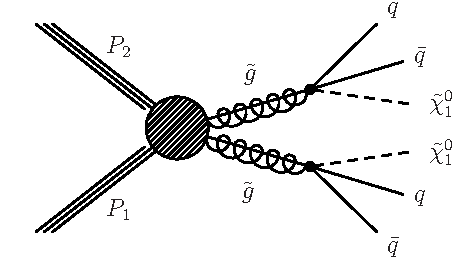
\includegraphics[width=7cm]{figures/Appendices/Ma5ValidationSUS13012/T1qqqq.pdf}
\caption{Diagram of the dominant SUSY production mechanism
for the T1qqqq signal model.}
\label{fig:T1qqqq}
\end{figure}

    \begin{table}[h!]
    \begin{centering}
    \begin{tabular}{  c | c | c  }
    \hline
    \hline	
    Cut Name & Official Count (Eff) & MA5 Count (Eff)\\
    \hline
        MET Cleaning & 190.6 (xxx) & 190.6 (xxx)\\
    No Lepton & 190.3 (99\%) & 190.6 (100\%)\\
    NJets$>$2 & 188.1 (98\%) & 188.49 (98\%)\\
    $H_T$$>$500 & 187.6 (99\%) & 188.07 (99\%)\\
    \MHT$>$200 & 158.7 (84\%) & 159.72 (84\%)\\
    Min $\Delta(\phi)$ & 130.8 (82\%) & 131.11 (82\%)\\
\hline
\hline
    \end{tabular}
    \caption{The cut flow for the baseline selection in CMS SUS-13-012 for
    the  T1qqqq working point $(m_{\tilde g},\,m_{\tilde\chi^0_1})=(1100,\,125)$~GeV. 
    The second column is the official account
    and our own results are given in column 3. The official counts are
    normalized to luminosity ${\cal L}=19.5$/fb and cross section $\sigma= 10.17$~pb, and our
    counts are normalized to match the official count after the first cut, MET
    Cleaning.}
    \label{table:CF1}
    \end{centering}
    \end{table}
    
    \begin{table}
    \begin{centering}
    \begin{tabular}{  l | c | c  }
    \hline
    \hline
    Signal Region Name & Official & MA5\\
    \hline
    NJets3-5,  $H_T$500-800,  \MHT200-300 & 1.4 & 1.21\\ 
 \hline 
NJets3-5,  $H_T$500-800,  \MHT300-450 & 2.4 & 2.08\\ 
 \hline 
NJets3-5,  $H_T$500-800,  \MHT450-600 & 1.7 & 1.36\\ 
 \hline 
NJets3-5,  $H_T$500-800,  \MHT$>$600 & 0.6 & 0.60\\ 
 \hline 
NJets3-5,  $H_T$800-1000,  \MHT200-300 & 2.1 & 1.81\\ 
 \hline 
NJets3-5,  $H_T$800-1000,  \MHT300-450 & 2.9 & 3.75\\ 
 \hline 
NJets3-5,  $H_T$800-1000,  \MHT450-600 & 4.2 & 3.74\\ 
 \hline 
NJets3-5,  $H_T$800-1000,  \MHT$>$600 & 4.1 & 4.04\\ 
 \hline 
NJets3-5,  $H_T$1000-1250,  \MHT200-300 & 4.2 & 3.70\\ 
 \hline 
NJets3-5,  $H_T$1000-1250,  \MHT300-450 & 8.1 & 6.93\\ 
 \hline 
NJets3-5,  $H_T$1000-1250,  \MHT450-600 & 7.6 & 7.18\\ 
 \hline 
NJets3-5,  $H_T$1000-1250,  \MHT$>$600 & 10.6 & 10.63\\ 
 \hline 
NJets3-5,  $H_T$1250-1500,  \MHT200-300 & 3.9 & 3.64\\ 
 \hline 
NJets3-5,  $H_T$1250-1500,  \MHT300-450 & 7.3 & 6.74\\ 
 \hline 
NJets3-5,  $H_T$1250-1500,  \MHT$>$450 & 15.6 & 16.52\\ 
 \hline 
NJets3-5,  $H_T$$>$1500,  \MHT200-300 & 4.5 & 4.41\\ 
 \hline 
NJets3-5,  $H_T$$>$1500,  \MHT$>$300 & 17.9 & 18.80\\ 
 \hline 
NJets6-7,  $H_T$500-800,  \MHT200-300 & 0.1 & 0.08\\ 
 \hline 
NJets6-7,  $H_T$500-800,  \MHT300-450 & 0.1 & 0.05\\ 
 \hline 
NJets6-7,  $H_T$500-800,  \MHT$>$450 & 0.1 & 0.04\\ 
 \hline 
NJets6-7,  $H_T$800-1000,  \MHT200-300 & 0.3 & 0.24\\ 
 \hline 
NJets6-7,  $H_T$800-1000,  \MHT300-450 & 0.6 & 0.51\\ 
 \hline 
NJets6-7,  $H_T$800-1000,  \MHT$>$450 & 0.8 & 0.71\\ 
 \hline 
NJets6-7,  $H_T$1000-1250,  \MHT200-300 & 0.9 & 0.91\\ 
 \hline 
NJets6-7,  $H_T$1000-1250,  \MHT300-450 & 1.8 & 1.74\\ 
 \hline 
NJets6-7,  $H_T$1000-1250,  \MHT$>$450 & 2.8 & 2.94\\ 
 \hline 
NJets6-7,  $H_T$1250-1500,  \MHT200-300 & 1.2 & 1.16\\ 
 \hline 
NJets6-7,  $H_T$1250-1500,  \MHT300-450 & 2.4 & 2.46\\ 
 \hline 
NJets6-7,  $H_T$1250-1500,  \MHT$>$450 & 4.1 & 5.16\\ 
 \hline 
NJets6-7,  $H_T$$>$1500,  \MHT200-300 & 2.3 & 2.56\\ 
 \hline 
NJets6-7,  $H_T$$>$1500,  \MHT$>$300 & 9.8 & 11.50\\ 
 \hline 
NJets$>$7,  $H_T$500-800,  \MHT$>$200 & 0.0 & 0.0\\ 
 \hline 
NJets$>$7,  $H_T$800-1000,  \MHT$>$200 & 0.0 & 0.01\\ 
 \hline 
NJets$>$7,  $H_T$1000-1250,  \MHT$>$200 & 0.2 & 0.28\\ 
 \hline 
NJets$>$7,  $H_T$1250-1500,  \MHT$>$200 & 0.5 & 0.75\\ 
 \hline 
NJets$>$7,  $H_T$$>$1500,  \MHT$>$200 & 2.2 & 2.69\\ 
 \hline 
\hline
    \end{tabular}
    \caption{The signal region (SR) counts in CMS SUS-13-012 for the T1qqqq scenario 
    after all selection has been applied. Column 2 is the official account obtained through generous correspondence with Christian Sanders,
    and our own results displayed in column 3. These counts were determined by applying the SR selection to the end of the cut flow featured in table \ref{table:CF1}.}
    \label{table:CF2}
    \end{centering}
    \end{table}
    
\begin{figure}
        \centering
        \subfloat[]{
                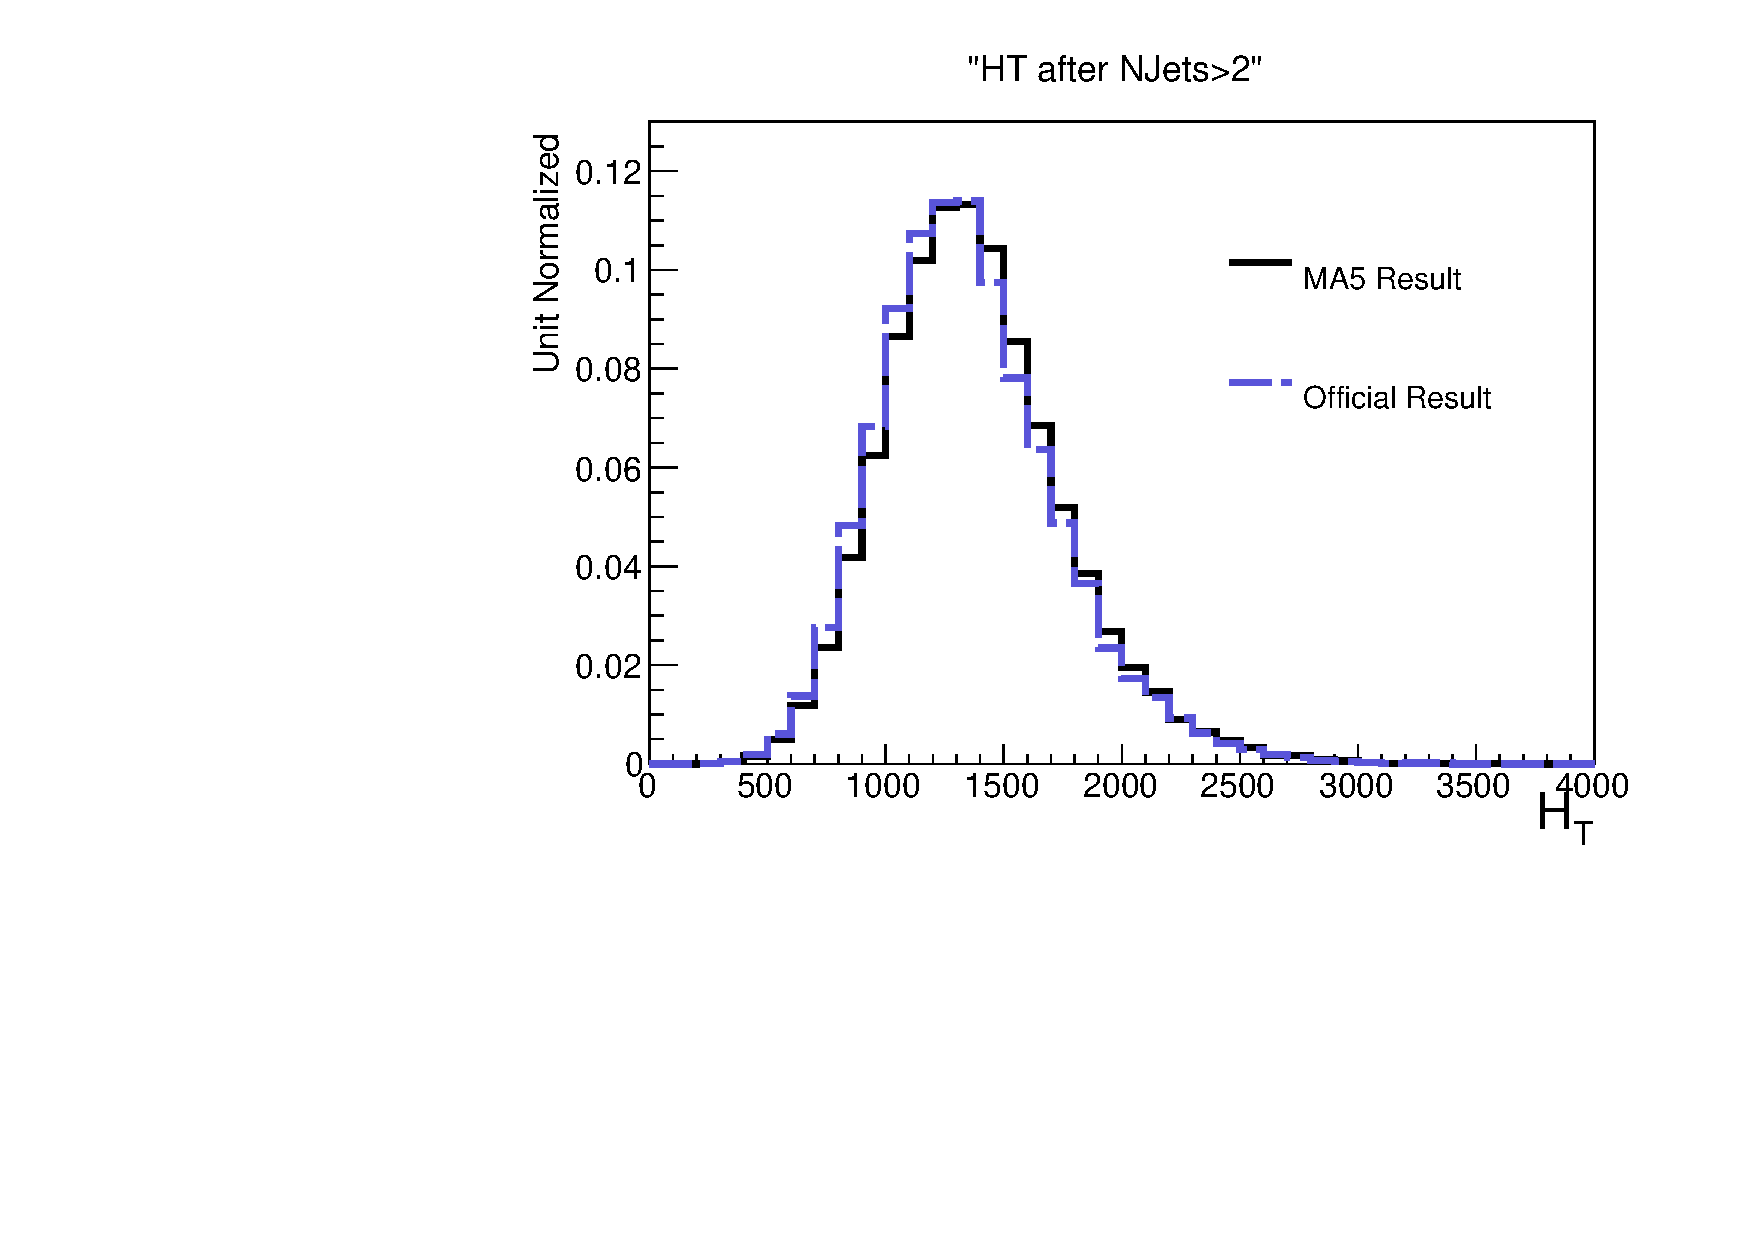
\includegraphics[width=0.5\textwidth]{figures/Appendices/Ma5ValidationSUS13012/T1qqqq_HT_after_NJets>2.pdf}
                \label{fig:gull}
        }%
        \hspace{-1 cm}
        ~ %add desired spacing between images, e. g. ~, \quad, \qquad, \hfill etc.
          %(or a blank line to force the subfigure onto a new line)
        \subfloat[]{
                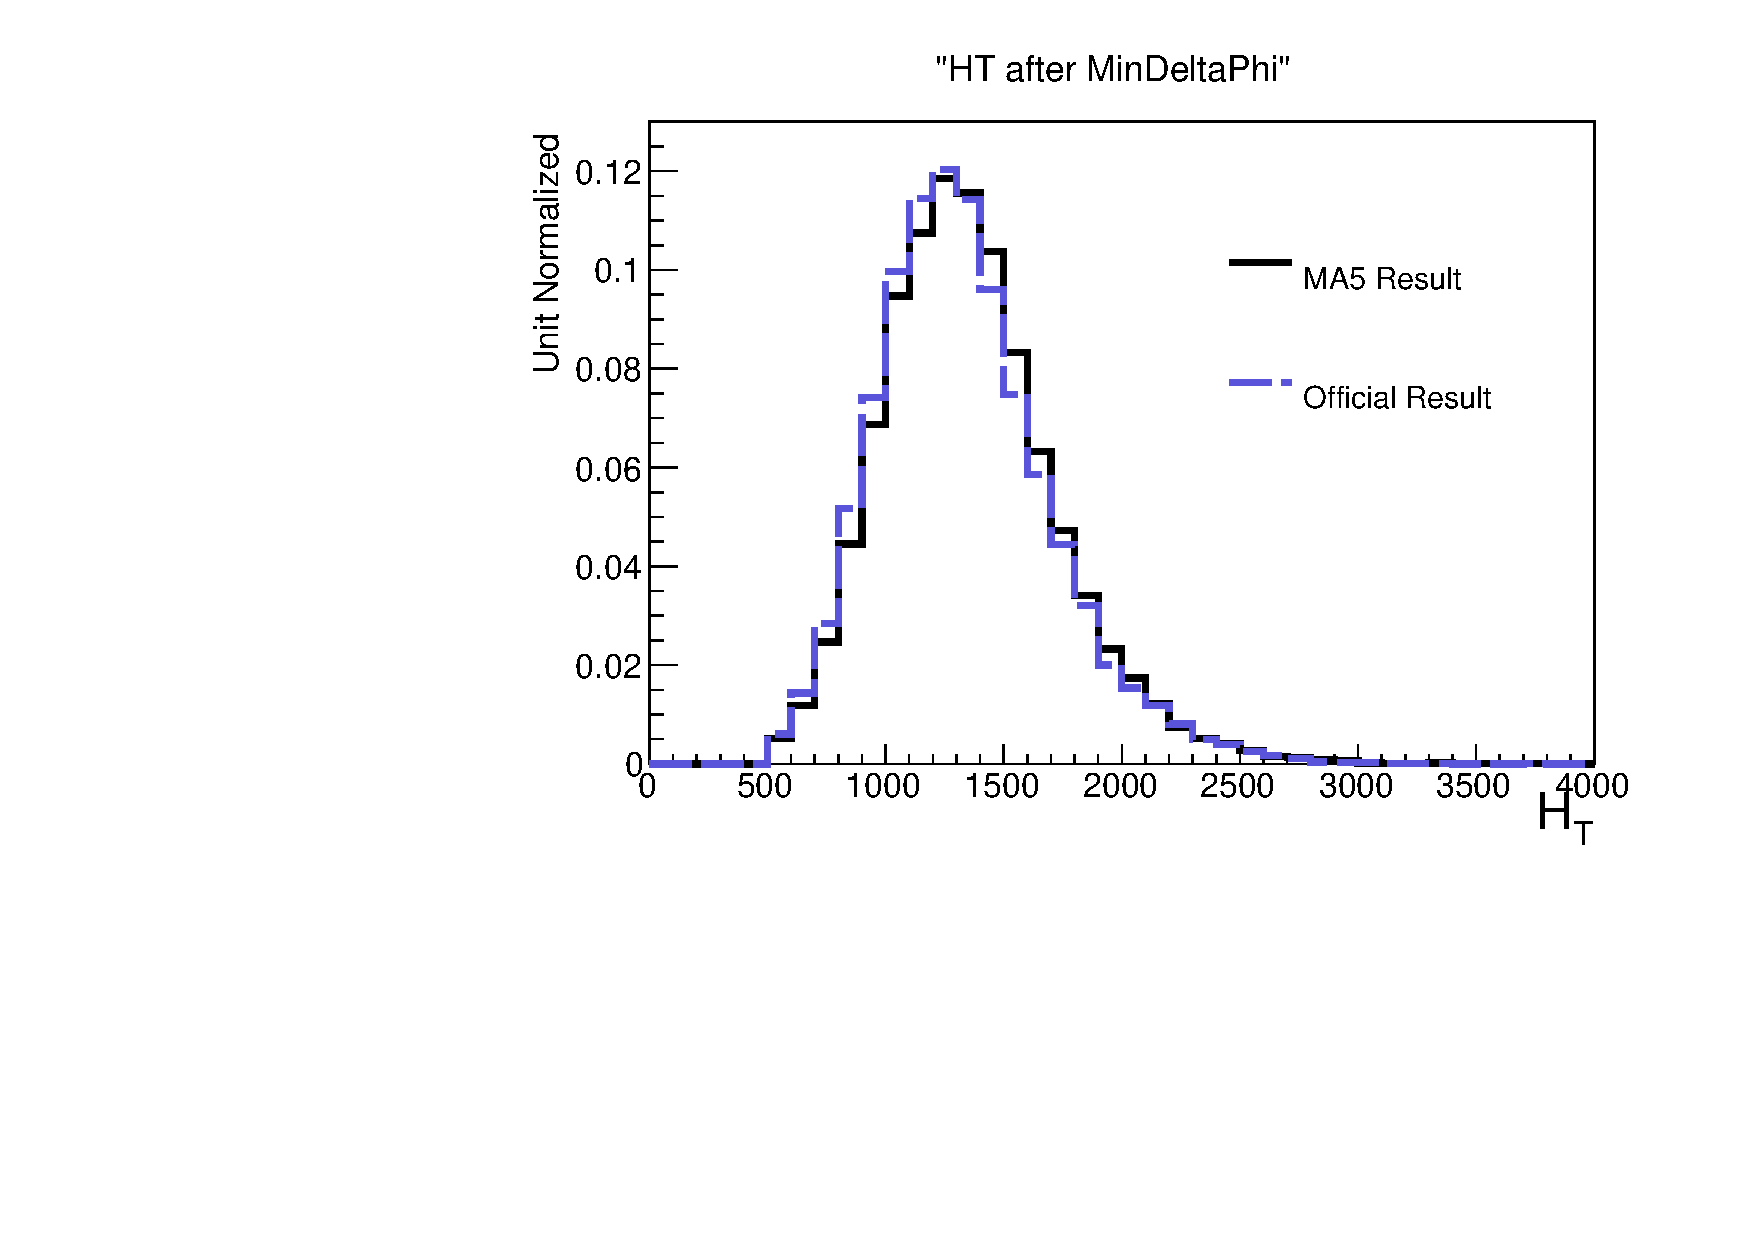
\includegraphics[width=0.5\textwidth]{figures/Appendices/Ma5ValidationSUS13012/T1qqqq_HT_after_MinDeltaPhi.pdf}
                \label{fig:tiger}
        }
        \caption{Comparison of the distributions of $H_T$ between the official and our own samples after the ``n-1" cut, Min $\Delta(\phi)$ (left), and after all baseline cuts (right), for the T1qqqq signal model.}\label{fig:animals}
\end{figure}        
        
\begin{figure}
        \centering
        \subfloat[]{
                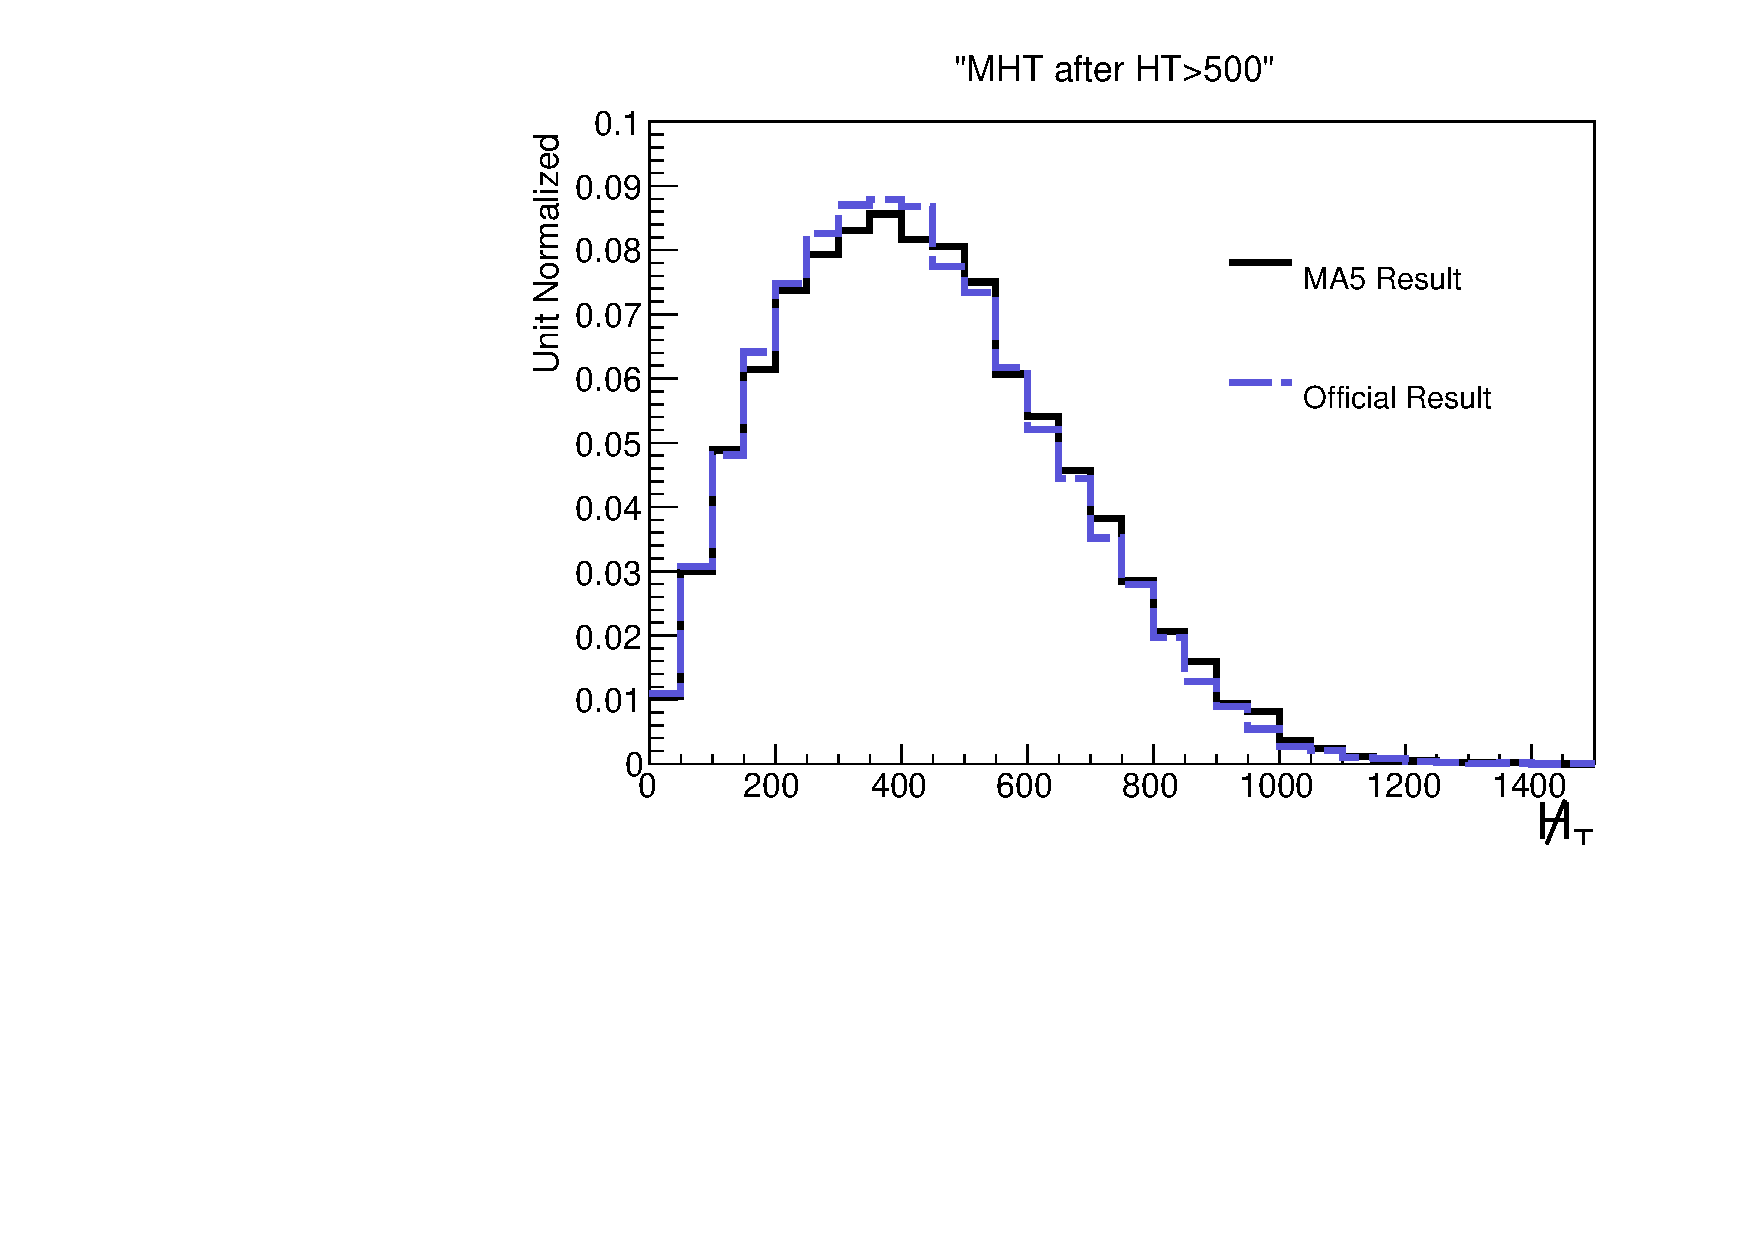
\includegraphics[width=0.5\textwidth]{figures/Appendices/Ma5ValidationSUS13012/T1qqqq_MHT_after_HT>500.pdf}
                \label{fig:gull}
        }%
        \hspace{-1 cm}
        ~ %add desired spacing between images, e. g. ~, \quad, \qquad, \hfill etc.
          %(or a blank line to force the subfigure onto a new line)
        \subfloat[]{
                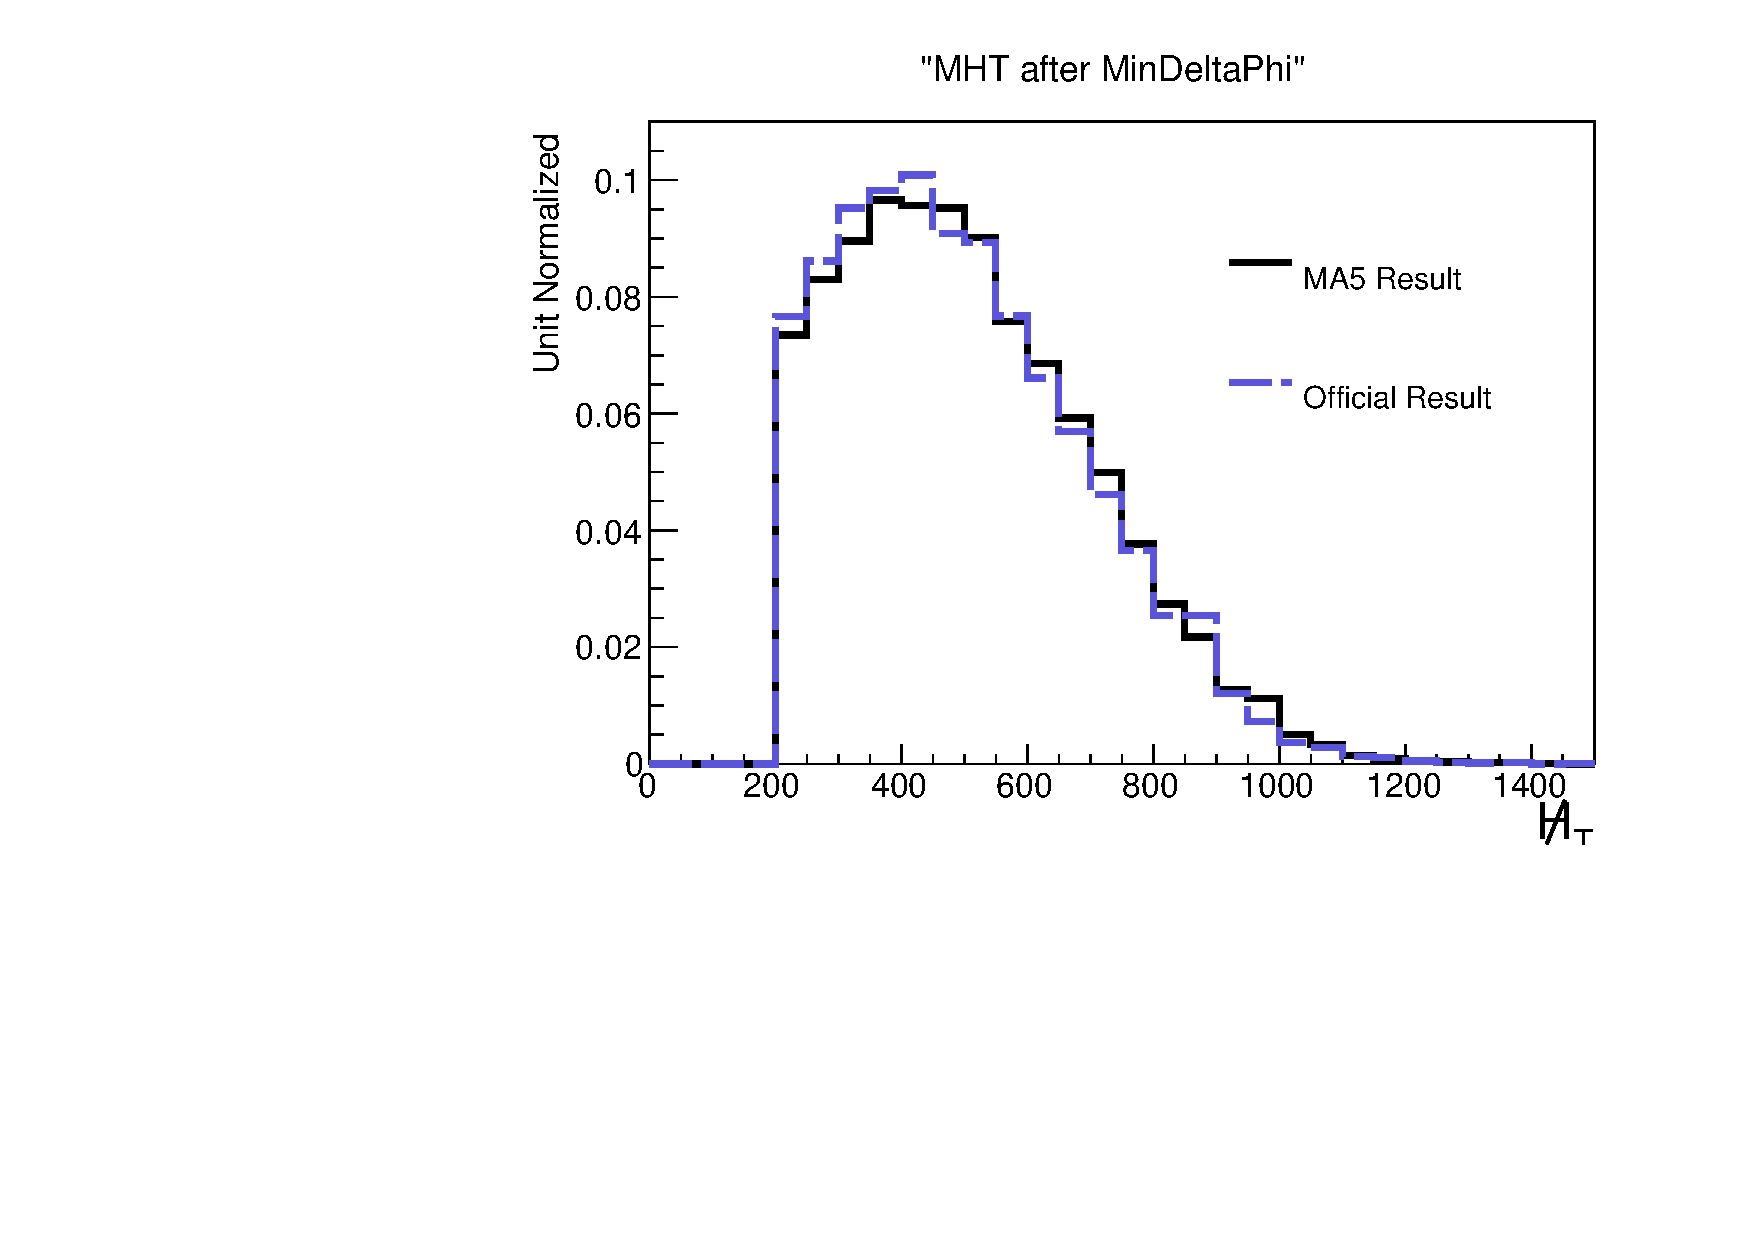
\includegraphics[width=0.5\textwidth]{figures/Appendices/Ma5ValidationSUS13012/T1qqqq_MHT_after_MinDeltaPhi.pdf}
                \label{fig:tiger}
        }
        \caption{Comparison of the distributions of \MHT between the official and our own samples after the ``n-1" cut, Min $\Delta(\phi)$ (left), and after all baseline cuts (right), for the T1qqqq signal model.}\label{fig:animals}
\end{figure}        
        
\begin{figure}
        \centering
        \subfloat[]{
                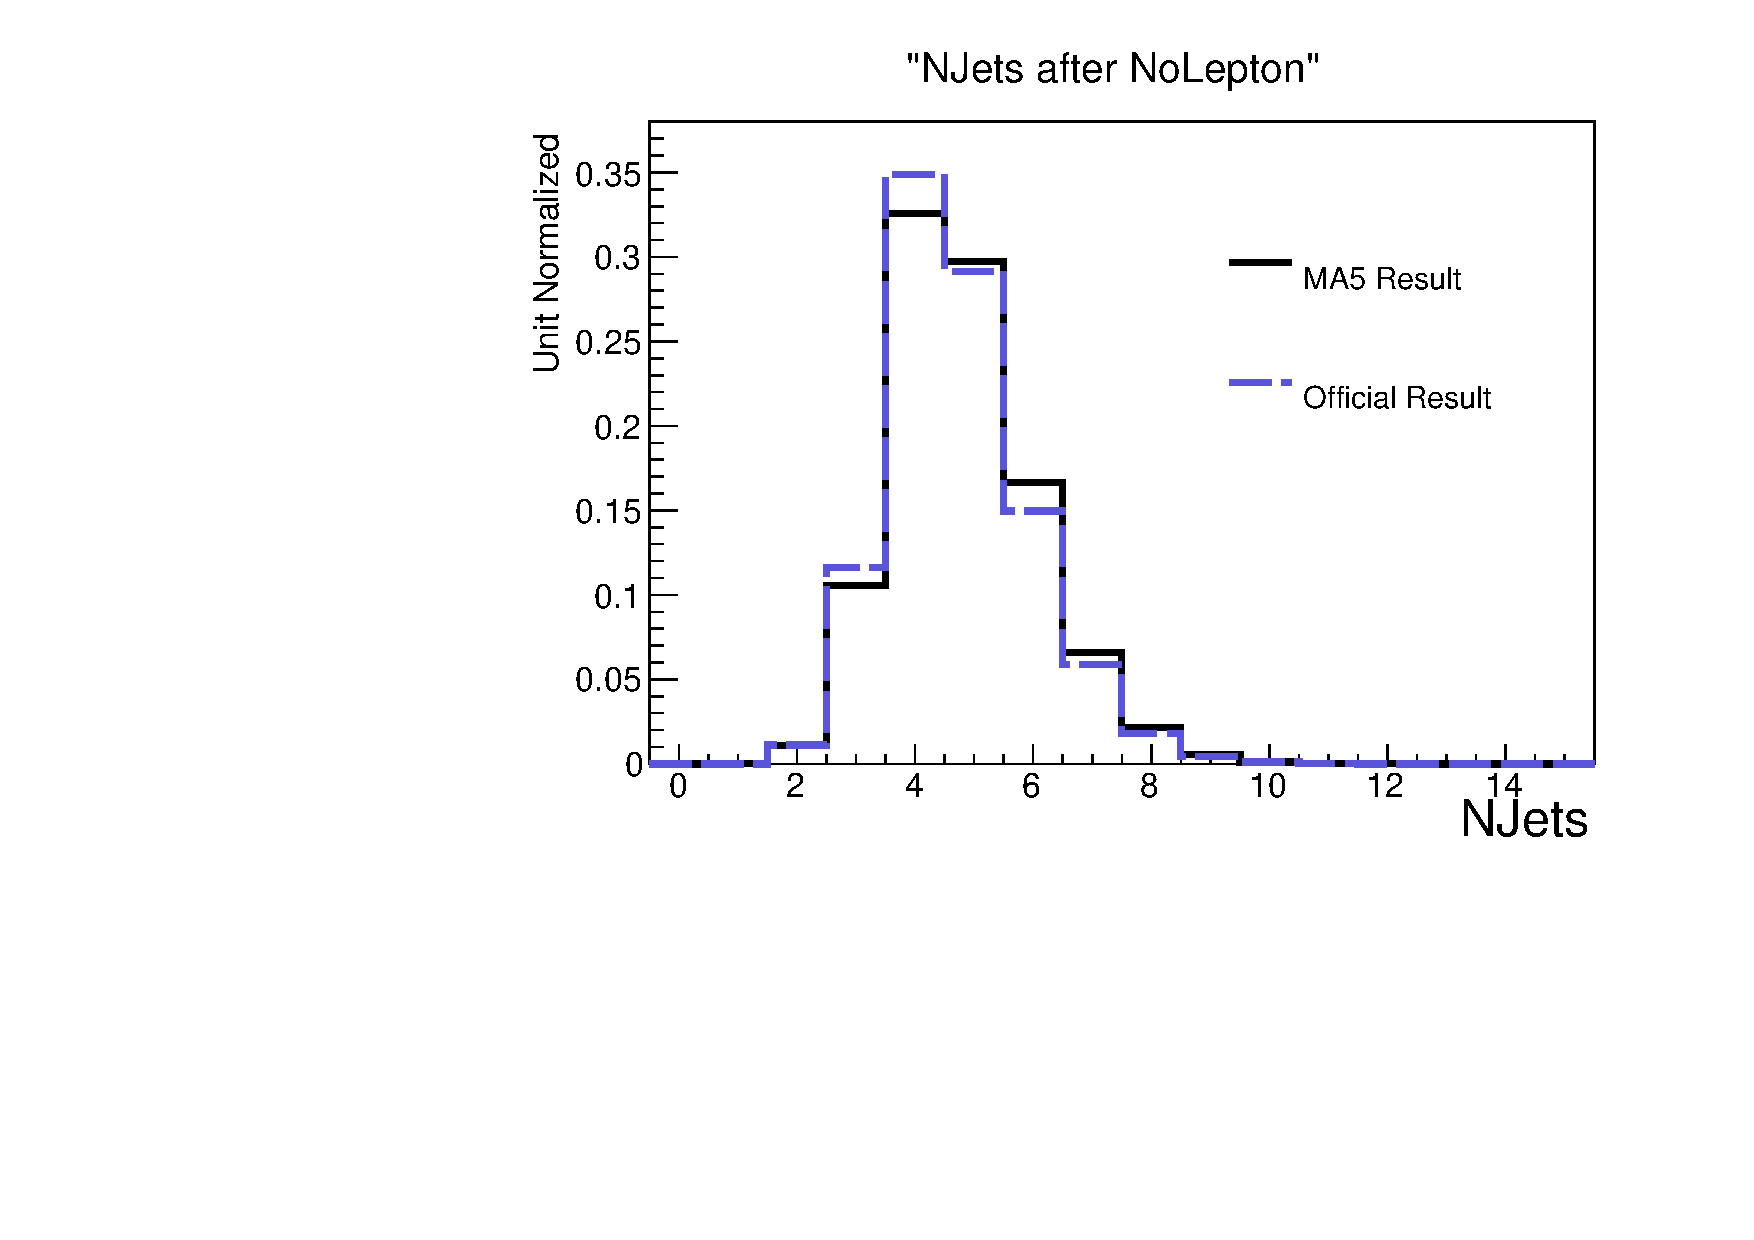
\includegraphics[width=0.5\textwidth]{figures/Appendices/Ma5ValidationSUS13012/T1qqqq_NJets_after_NoLepton.pdf}
                \label{fig:gull}
        }%
        \hspace{-1 cm}
        ~ %add desired spacing between images, e. g. ~, \quad, \qquad, \hfill etc.
          %(or a blank line to force the subfigure onto a new line)
        \subfloat[]{
                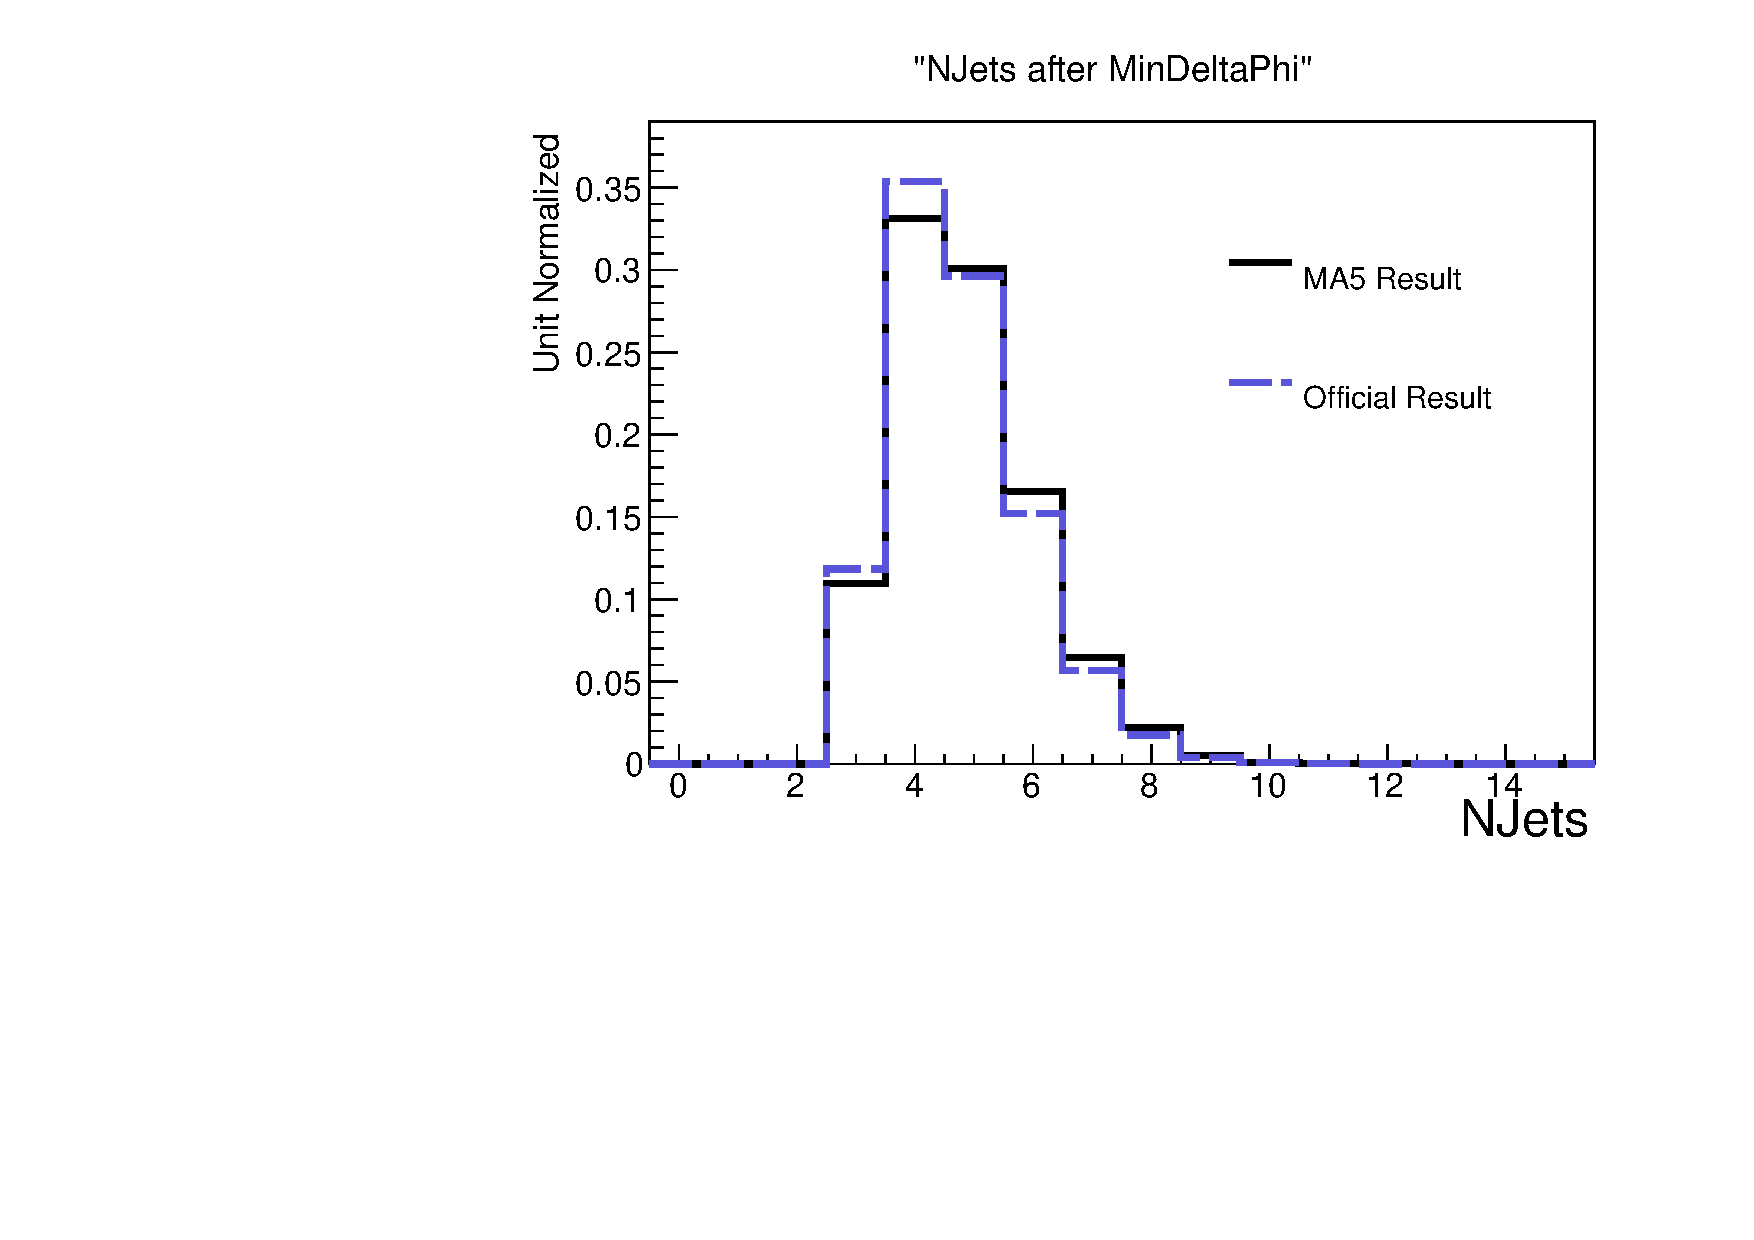
\includegraphics[width=0.5\textwidth]{figures/Appendices/Ma5ValidationSUS13012/T1qqqq_NJets_after_MinDeltaPhi.pdf}
                \label{fig:tiger}
        }
        \caption{Comparison of the distributions of NJets between the official and our own samples after the ``n-1" cut, Min $\Delta(\phi)$ (left), and after all baseline cuts (right), for the T1qqqq signal model.}\label{fig:animals}
\end{figure}        
        
        \begin{figure}
        \centering
        \subfloat[]{
        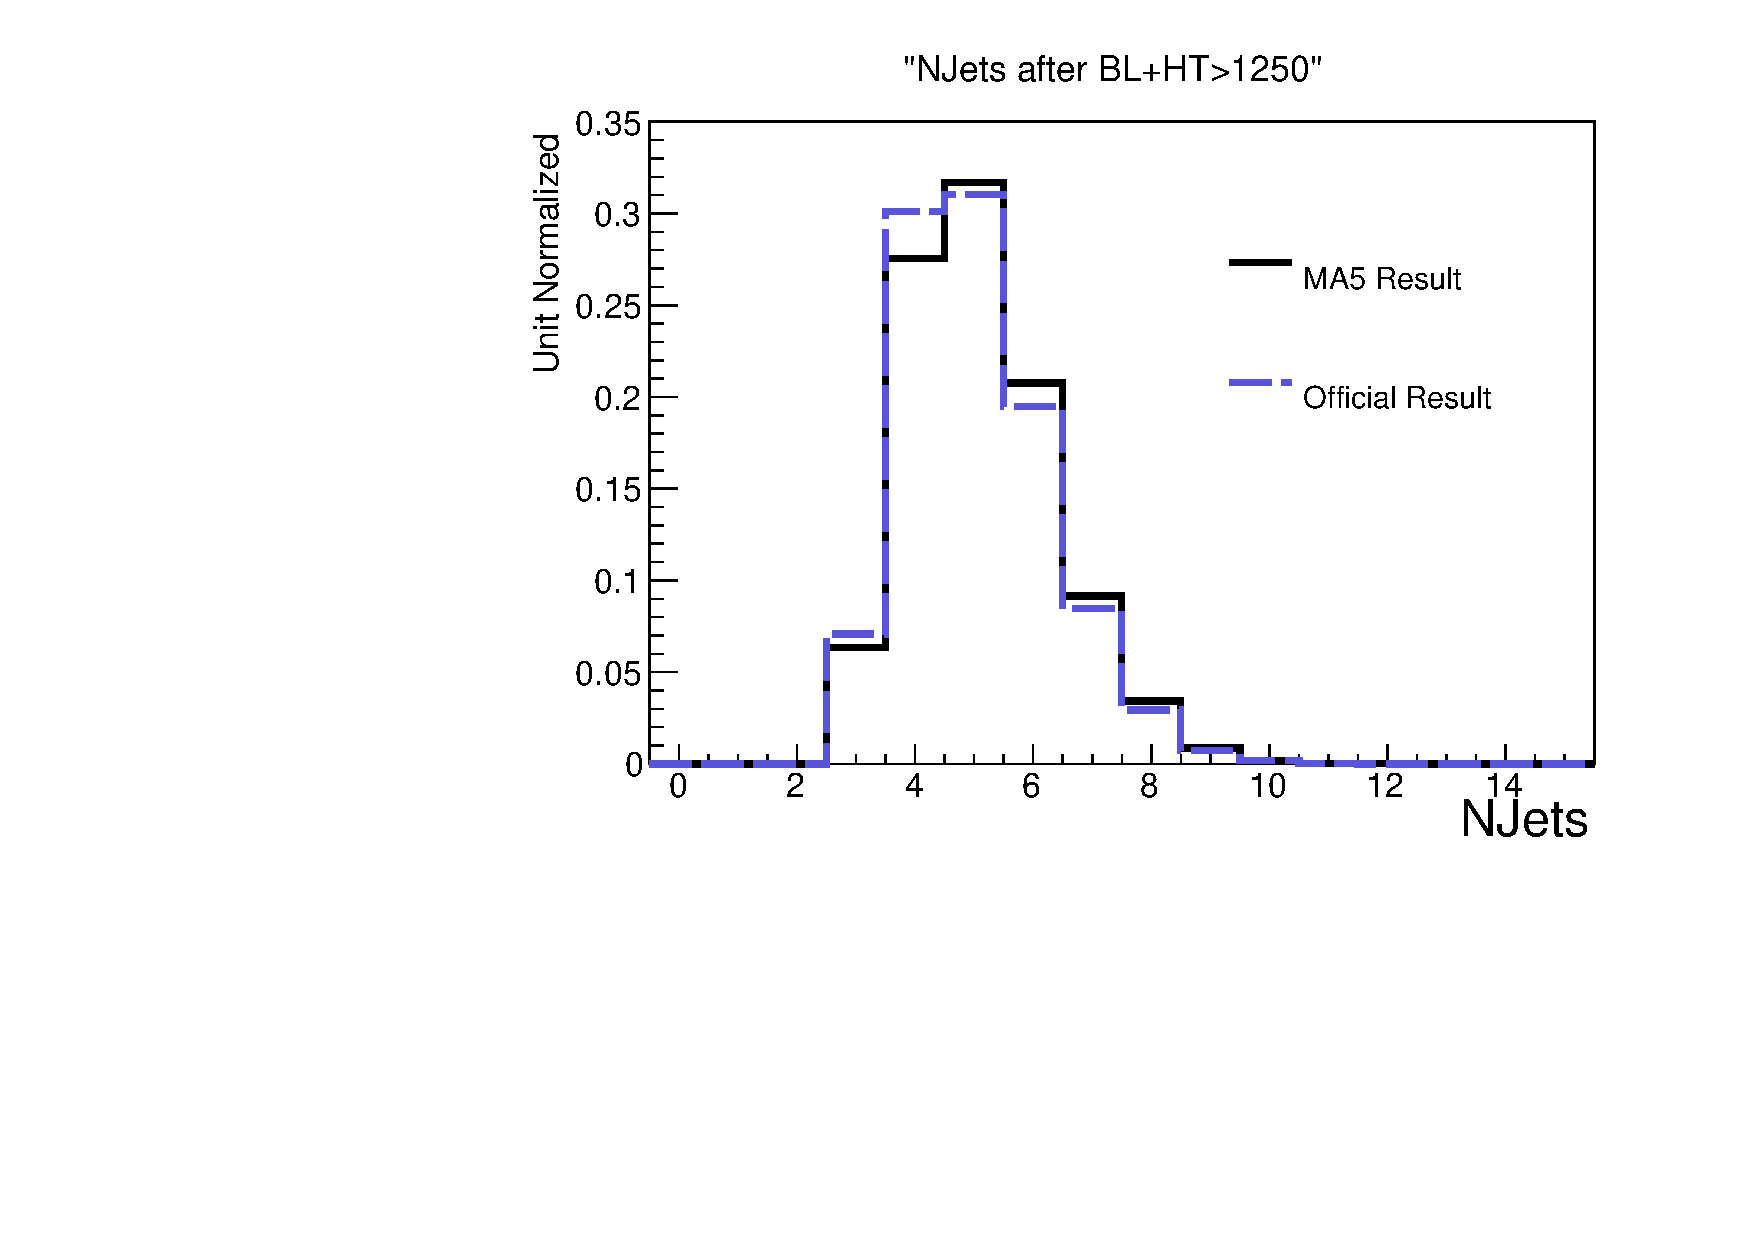
\includegraphics[width=0.5\textwidth]{figures/Appendices/Ma5ValidationSUS13012/T1qqqq_NJets_after_BL+HT>1250.pdf}
        \label{fig:gull}
        }%
        \hspace{-1 cm}
        ~ %add desired spacing between images, e. g. ~, \quad, \qquad, \hfill etc.
        %(or a blank line to force the subfigure onto a new line)
        \subfloat[]{
        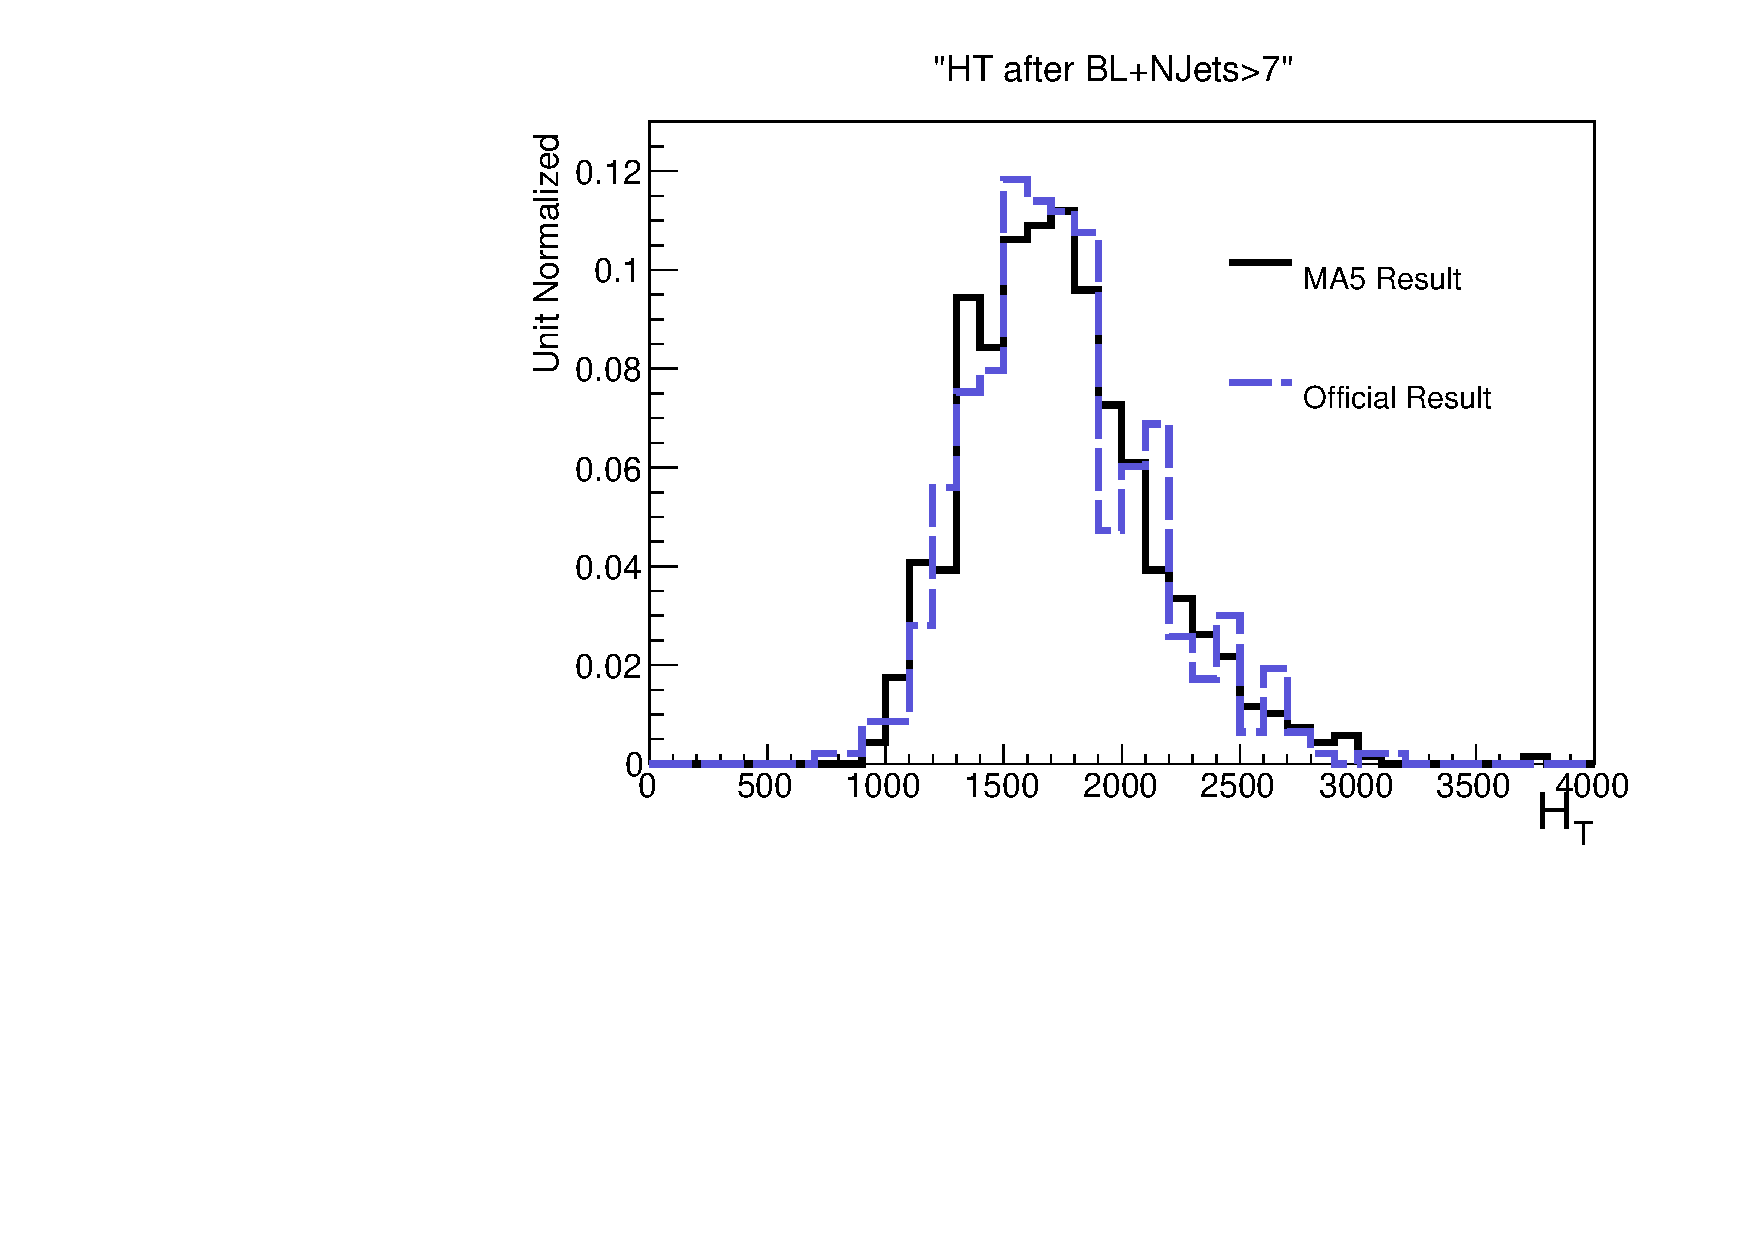
\includegraphics[width=0.5\textwidth]{figures/Appendices/Ma5ValidationSUS13012/T1qqqq_HT_after_BL+NJets>7.pdf}
        \label{fig:tiger}
        }
        \caption{Additional checks: comparison between ours and the official distributions of NJets after BL+$H_T$$>$1250 cuts (left), and $H_T$ after BL+NJets$>$7 cuts (right), for the T1qqqq signal model.}
        \end{figure}        

\clearpage
%%%%%%%%%%%%%%%%%%%%%%%%%%%%%%%%%%%%%%%%%%%%%%%%%
\subsubsection{T1tttt simplified model}
%%%%%%%%%%%%%%%%%%%%%%%%%%%%%%%%%%%%%%%%%%%%%%%%%

\begin{figure}[h!]
\centering
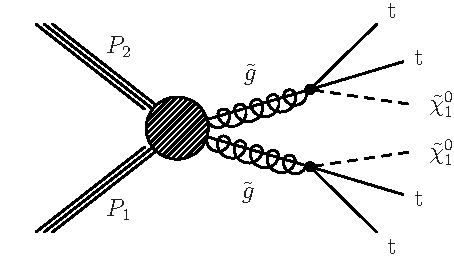
\includegraphics[width=7cm]{figures/Appendices/Ma5ValidationSUS13012/T1tttt.pdf}
\caption{Diagram of the dominant SUSY production mechanism
for the T1tttt signal model.}
\label{fig:T1tttt}
\end{figure}

    \begin{table}[h!]
    \begin{centering}
    \begin{tabular}{  c | c | c  }
    \hline
    \hline
    Cut Name & Official Count (Eff) & MA5 Count (Eff)\\
    \hline
        MET Cleaning & 190.5 (xxx) & 190.5 (xxx)\\
    No Lepton & 95.9 (50\%) & 101.04 (53\%)\\
    NJets$>$2 & 95.8 (99\%) & 100.87 (99\%)\\
    $H_T$$>$500 & 95.1 (99\%) & 100.01 (99\%)\\
    \MHT$>$200 & 75.4 (79\%) & 81.23 (81\%)\\
    Min $\Delta(\phi)$ & 62.3 (82\%) & 66.92 (82\%)\\
\hline
\hline
    \end{tabular}
    \caption{The cut flow for the baseline selection in CMS SUS-13-012 for
    the T1tttt working point $(m_{\tilde g},\,m_{\tilde\chi^0_1})=(1100,\,125)$~GeV.  
    The second column is the official account
    and our own results are given in column 3. The official counts are
    normalized to luminosity ${\cal L}=19.5$/fb and cross section $\sigma= 10.17$~pb, and our
    counts are normalized to match the official count after the first cut, MET
    Cleaning.}
    \label{table:CF2}
    \end{centering}
    \end{table}
    
    \begin{table}
    \begin{centering}
    \begin{tabular}{  l | c | c  }
    \hline
    \hline
    Signal Region Name & Official & MA5\\
    \hline
    NJets3-5,  $H_T$500-800,  \MHT200-300 & 0.8 & 0.85\\ 
 \hline 
NJets3-5,  $H_T$500-800,  \MHT300-450 & 1.4 & 1.22\\ 
 \hline 
NJets3-5,  $H_T$500-800,  \MHT450-600 & 0.8 & 0.85\\ 
 \hline 
NJets3-5,  $H_T$500-800,  \MHT$>$600 & 0.2 & 0.31\\ 
 \hline 
NJets3-5,  $H_T$800-1000,  \MHT200-300 & 0.5 & 0.45\\ 
 \hline 
NJets3-5,  $H_T$800-1000,  \MHT300-450 & 0.7 & 1.00\\ 
 \hline 
NJets3-5,  $H_T$800-1000,  \MHT450-600 & 1.0 & 1.03\\ 
 \hline 
NJets3-5,  $H_T$800-1000,  \MHT$>$600 & 0.8 & 0.79\\ 
 \hline 
NJets3-5,  $H_T$1000-1250,  \MHT200-300 & 0.5 & 0.53\\ 
 \hline 
NJets3-5,  $H_T$1000-1250,  \MHT300-450 & 1.0 & 0.83\\ 
 \hline 
NJets3-5,  $H_T$1000-1250,  \MHT450-600 & 0.8 & 0.87\\ 
 \hline 
NJets3-5,  $H_T$1000-1250,  \MHT$>$600 & 0.9 & 1.01\\ 
 \hline 
NJets3-5,  $H_T$1250-1500,  \MHT200-300 & 0.4 & 0.40\\ 
 \hline 
NJets3-5,  $H_T$1250-1500,  \MHT300-450 & 0.5 & 0.58\\ 
 \hline 
NJets3-5,  $H_T$1250-1500,  \MHT$>$450 & 0.8 & 0.81\\ 
 \hline 
NJets3-5,  $H_T$$>$1500,  \MHT200-300 & 0.3 & 0.34\\ 
 \hline 
NJets3-5,  $H_T$$>$1500,  \MHT$>$300 & 0.9 & 1.01\\ 
 \hline 
NJets6-7,  $H_T$500-800,  \MHT200-300 & 0.9 & 0.81\\ 
 \hline 
NJets6-7,  $H_T$500-800,  \MHT300-450 & 1.2 & 0.85\\ 
 \hline 
NJets6-7,  $H_T$500-800,  \MHT$>$450 & 0.6 & 0.44\\ 
 \hline 
NJets6-7,  $H_T$800-1000,  \MHT200-300 & 1.5 & 1.16\\ 
 \hline 
NJets6-7,  $H_T$800-1000,  \MHT300-450 & 2.5 & 2.35\\ 
 \hline 
NJets6-7,  $H_T$800-1000,  \MHT$>$450 & 2.5 & 2.59\\ 
 \hline 
NJets6-7,  $H_T$1000-1250,  \MHT200-300 & 1.8 & 1.71\\ 
 \hline 
NJets6-7,  $H_T$1000-1250,  \MHT300-450 & 3.4 & 3.37\\ 
 \hline 
NJets6-7,  $H_T$1000-1250,  \MHT$>$450 & 4.5 & 5.21\\ 
 \hline 
NJets6-7,  $H_T$1250-1500,  \MHT200-300 & 1.4 & 1.46\\ 
 \hline 
NJets6-7,  $H_T$1250-1500,  \MHT300-450 & 2.2 & 2.43\\ 
 \hline 
NJets6-7,  $H_T$1250-1500,  \MHT$>$450 & 2.8 & 3.34\\ 
 \hline 
NJets6-7,  $H_T$$>$1500,  \MHT200-300 & 1.1 & 1.16\\ 
 \hline 
NJets6-7,  $H_T$$>$1500,  \MHT$>$300 & 3.4 & 3.99\\ 
 \hline 
NJets$>$7,  $H_T$500-800,  \MHT$>$200 & 0.2 & 0.15\\ 
 \hline 
NJets$>$7,  $H_T$800-1000,  \MHT$>$200 & 1.9 & 1.69\\ 
 \hline 
NJets$>$7,  $H_T$1000-1250,  \MHT$>$200 & 5.7 & 6.37\\ 
 \hline 
NJets$>$7,  $H_T$1250-1500,  \MHT$>$200 & 5.9 & 7.28\\ 
 \hline 
NJets$>$7,  $H_T$$>$1500,  \MHT$>$200 & 6.0 & 7.53\\ 
 \hline 
\hline
    \end{tabular}
    \caption{The signal region (SR) counts in CMS SUS-13-012 for the T1tttt scenario 
    after all selection has been applied. Column 2 is the official account obtained through generous correspondence with Christian Sanders,
    and our own results displayed in column 3. These counts were determined by applying the SR selection to the end of the cut flow featured in table \ref{table:CF2}.}
    \end{centering}
    \end{table}
    
\begin{figure}
        \centering
        \subfloat[]{
                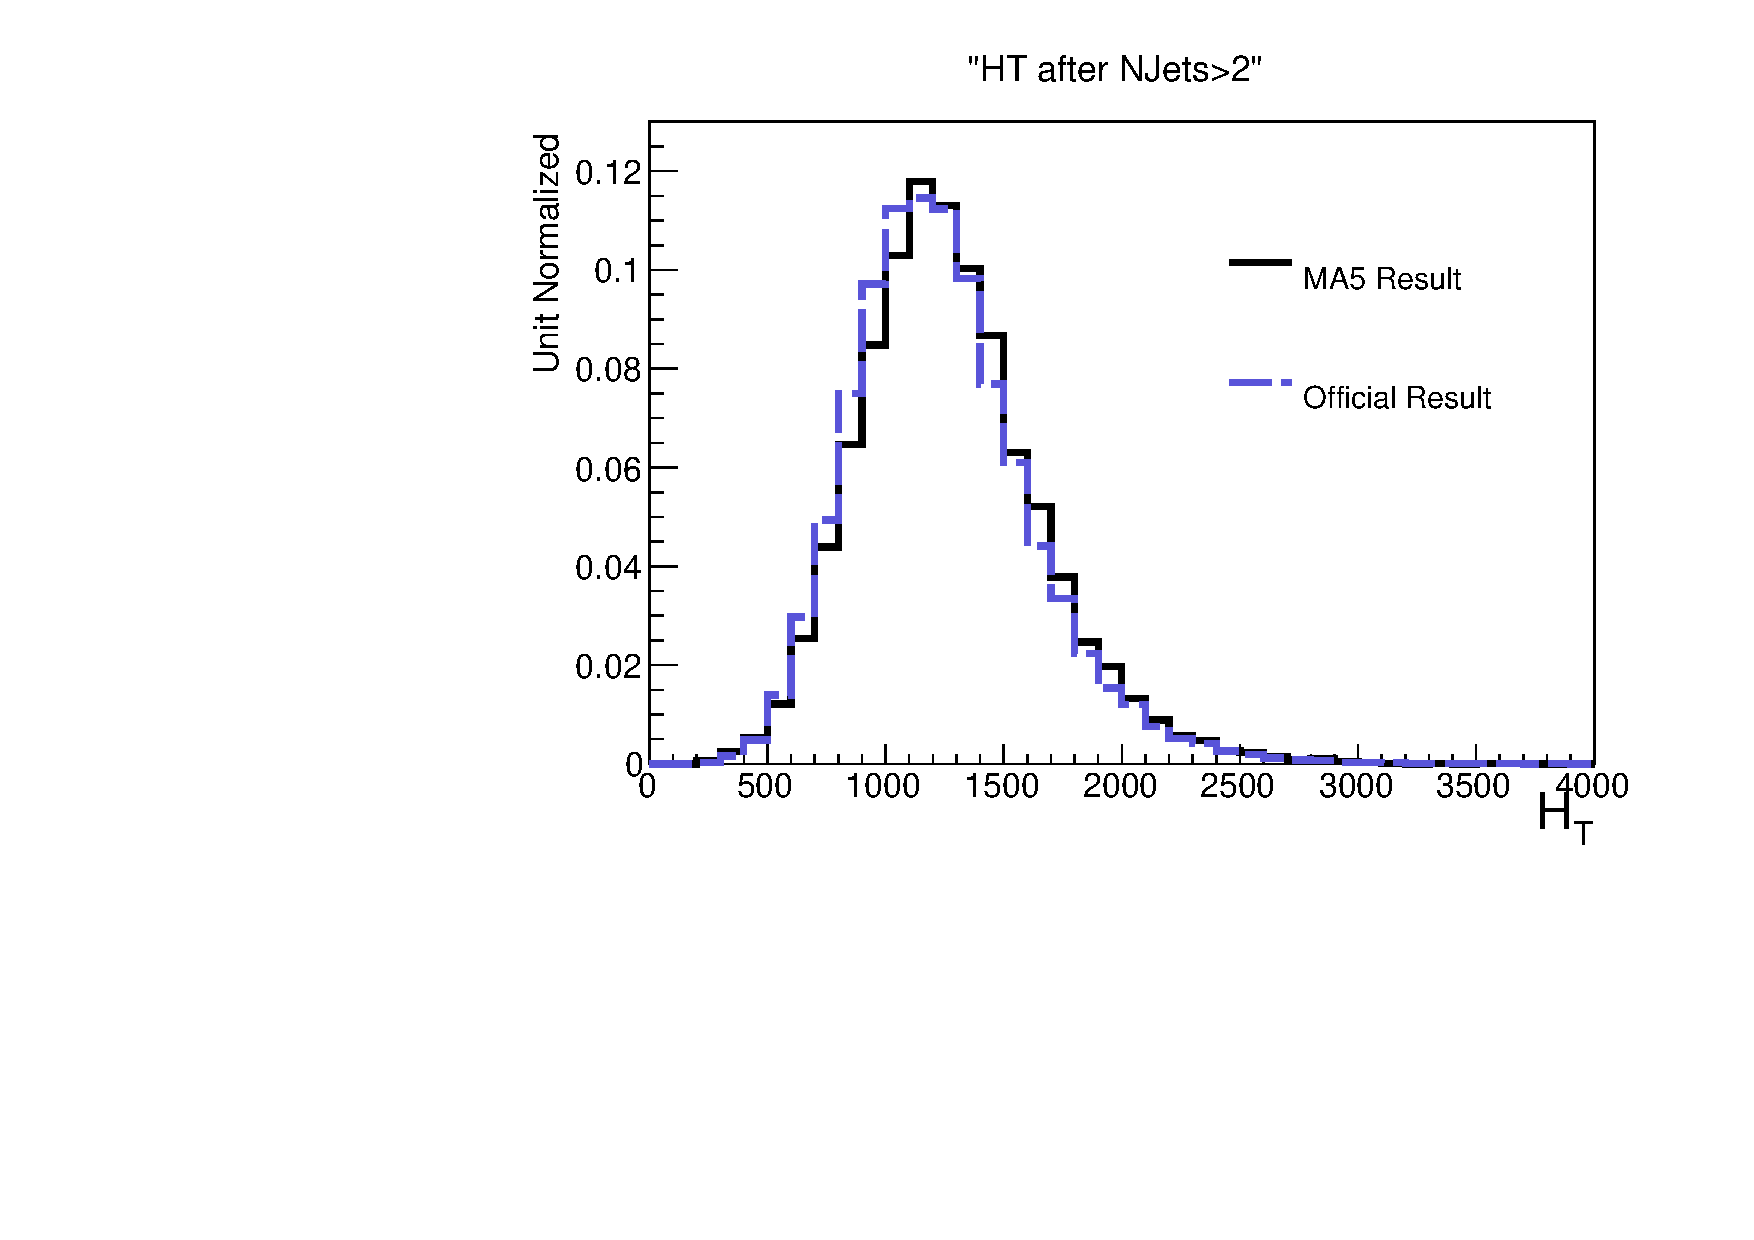
\includegraphics[width=0.5\textwidth]{figures/Appendices/Ma5ValidationSUS13012/T1tttt_HT_after_NJets>2.pdf}
                \label{fig:gull}
        }%
        \hspace{-1 cm}
        ~ %add desired spacing between images, e. g. ~, \quad, \qquad, \hfill etc.
          %(or a blank line to force the subfigure onto a new line)
        \subfloat[]{
                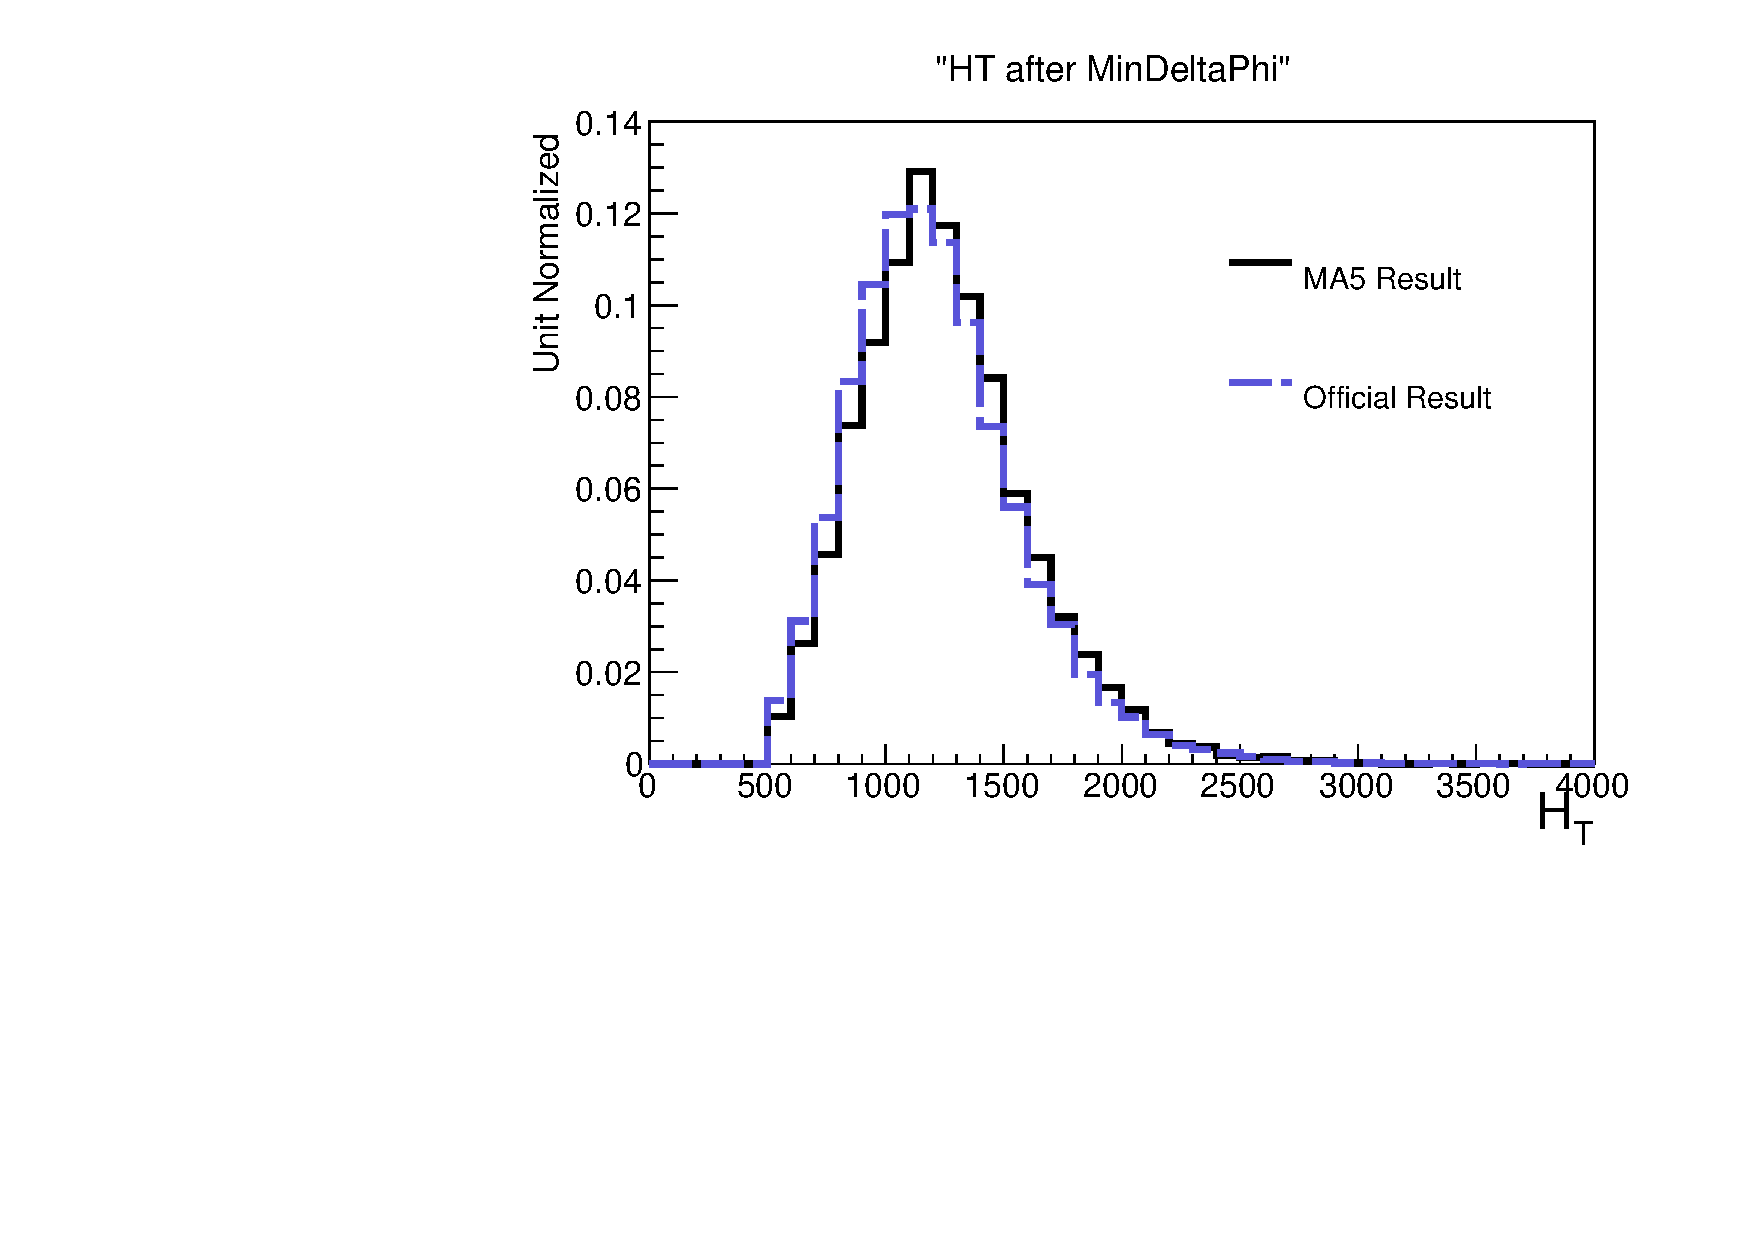
\includegraphics[width=0.5\textwidth]{figures/Appendices/Ma5ValidationSUS13012/T1tttt_HT_after_MinDeltaPhi.pdf}
                \label{fig:tiger}
        }
        \caption{Comparison of the distributions of $H_T$ between the official and our own samples after the ``n-1" cut, Min $\Delta(\phi)$ (left), and after all baseline cuts (right), for the T1tttt signal model.}\label{fig:animals}
\end{figure}        
        
\begin{figure}
        \centering
        \subfloat[]{
                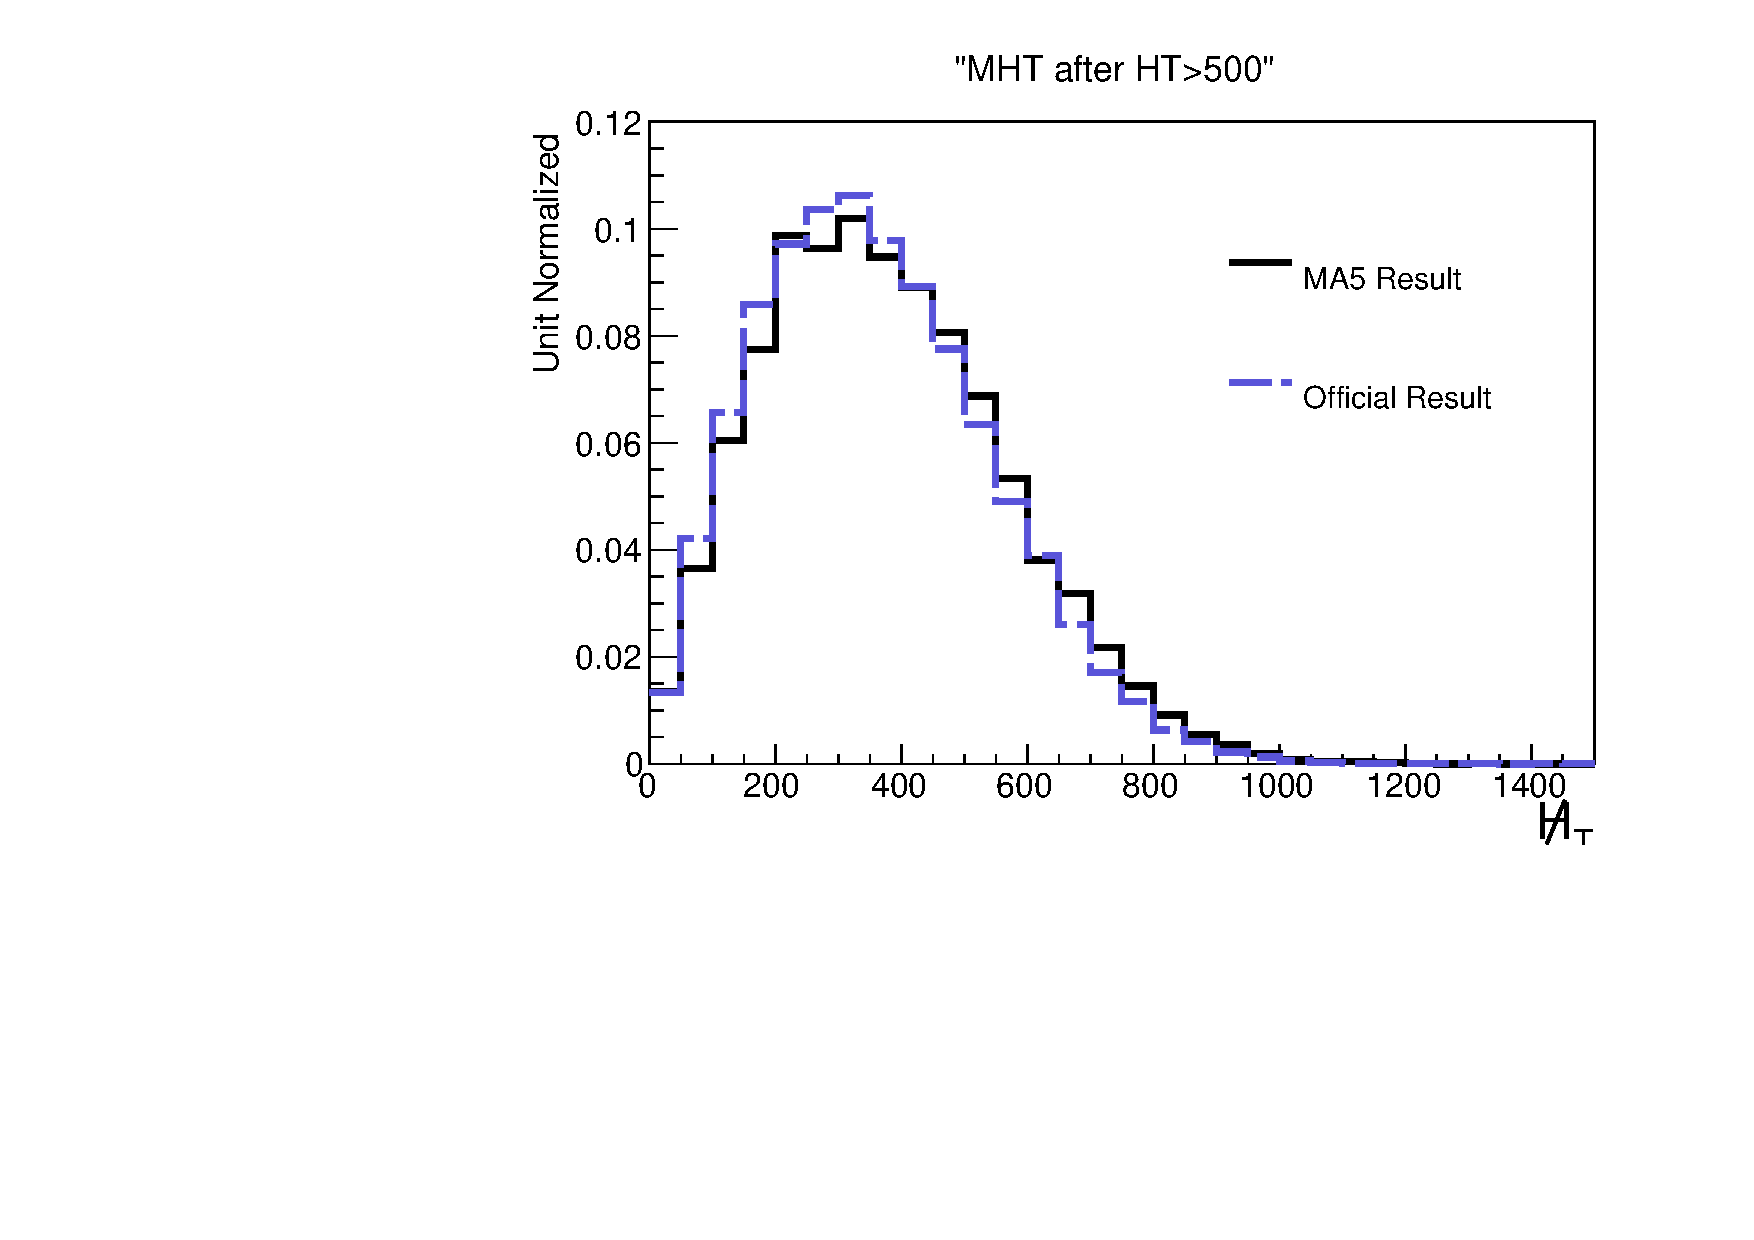
\includegraphics[width=0.5\textwidth]{figures/Appendices/Ma5ValidationSUS13012/T1tttt_MHT_after_HT>500.pdf}
                \label{fig:gull}
        }%
        \hspace{-1 cm}
        ~ %add desired spacing between images, e. g. ~, \quad, \qquad, \hfill etc.
          %(or a blank line to force the subfigure onto a new line)
        \subfloat[]{
                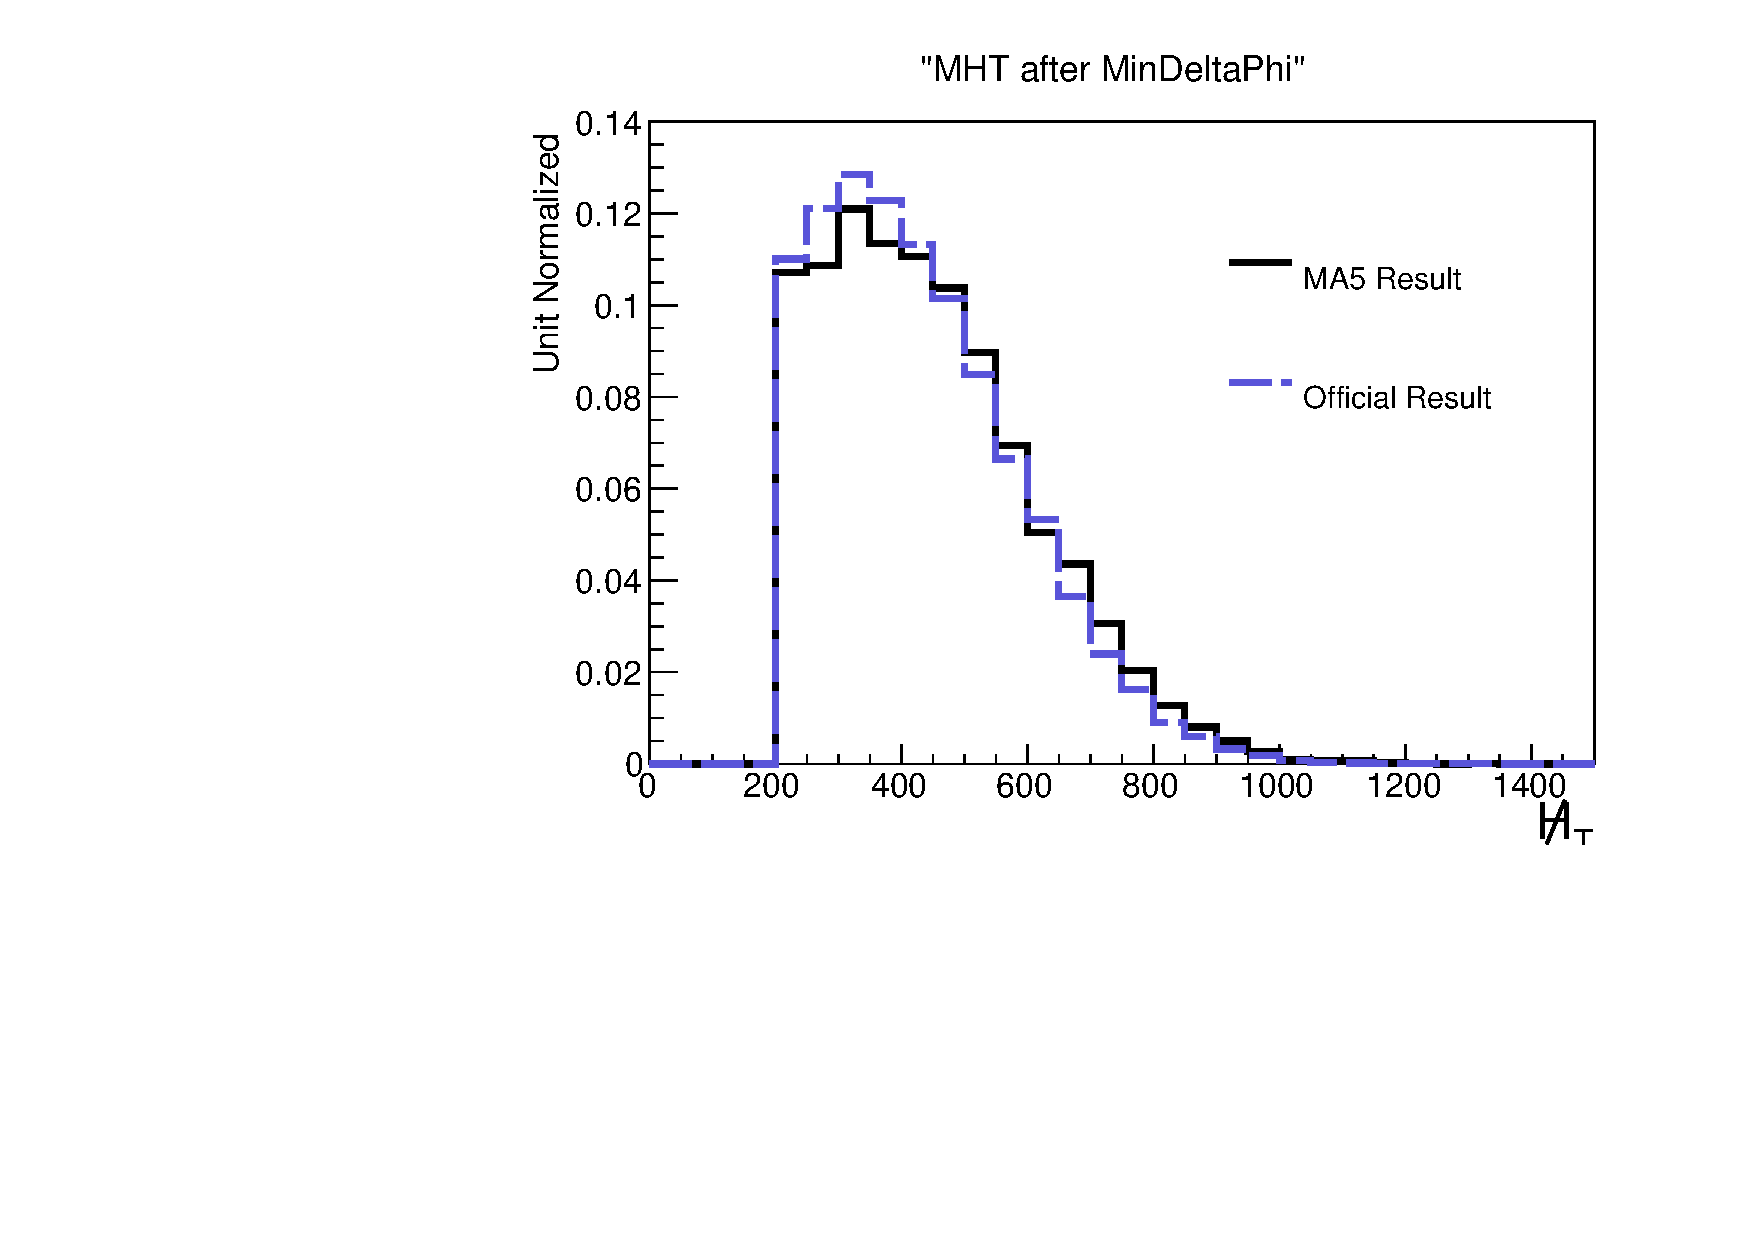
\includegraphics[width=0.5\textwidth]{figures/Appendices/Ma5ValidationSUS13012/T1tttt_MHT_after_MinDeltaPhi.pdf}
                \label{fig:tiger}
        }
        \caption{Comparison of the distributions of \MHT between the official and our own samples after the ``n-1" cut, Min $\Delta(\phi)$ (left), and after all baseline cuts (right), for the T1tttt signal model.}\label{fig:animals}
\end{figure}        
        
\begin{figure}
        \centering
        \subfloat[]{
                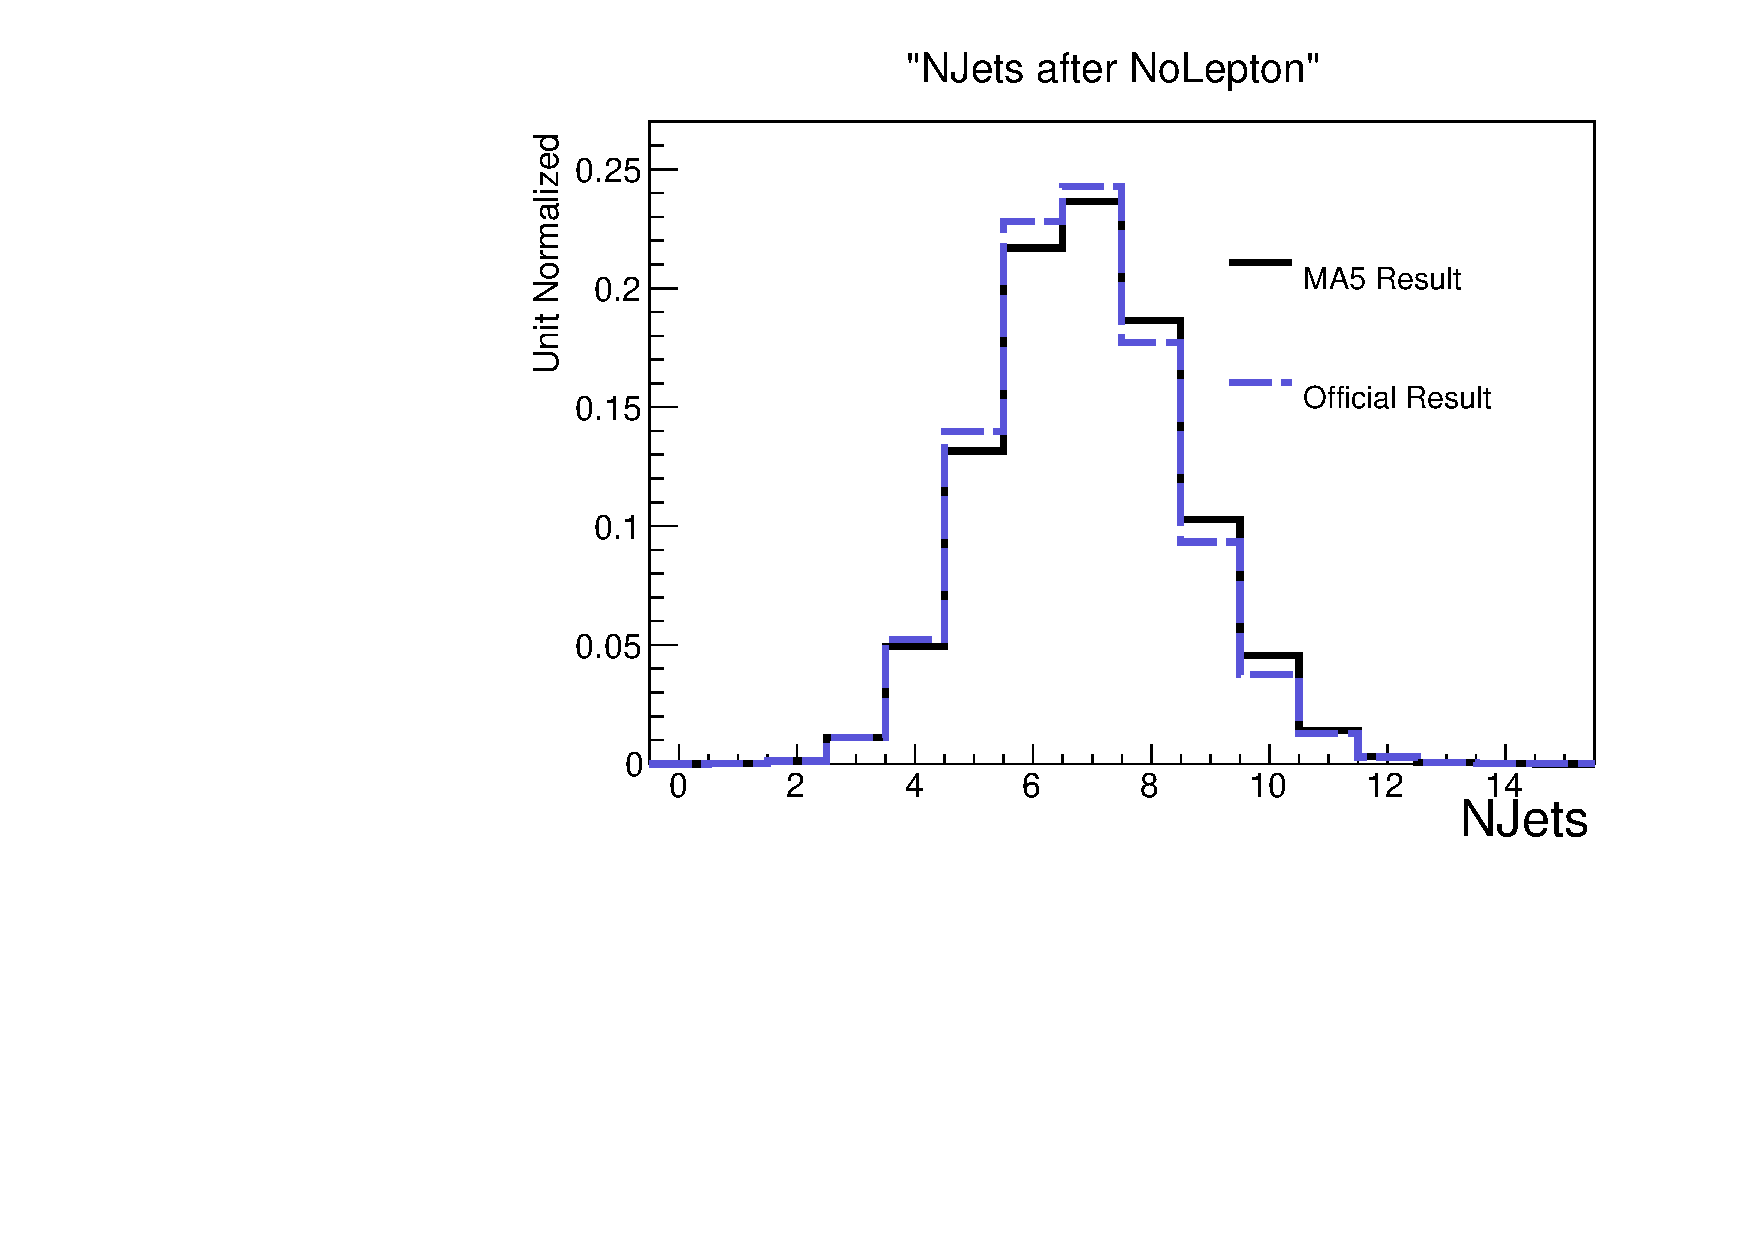
\includegraphics[width=0.5\textwidth]{figures/Appendices/Ma5ValidationSUS13012/T1tttt_NJets_after_NoLepton.pdf}
                \label{fig:gull}
        }%
        \hspace{-1 cm}
        ~ %add desired spacing between images, e. g. ~, \quad, \qquad, \hfill etc.
          %(or a blank line to force the subfigure onto a new line)
        \subfloat[]{
                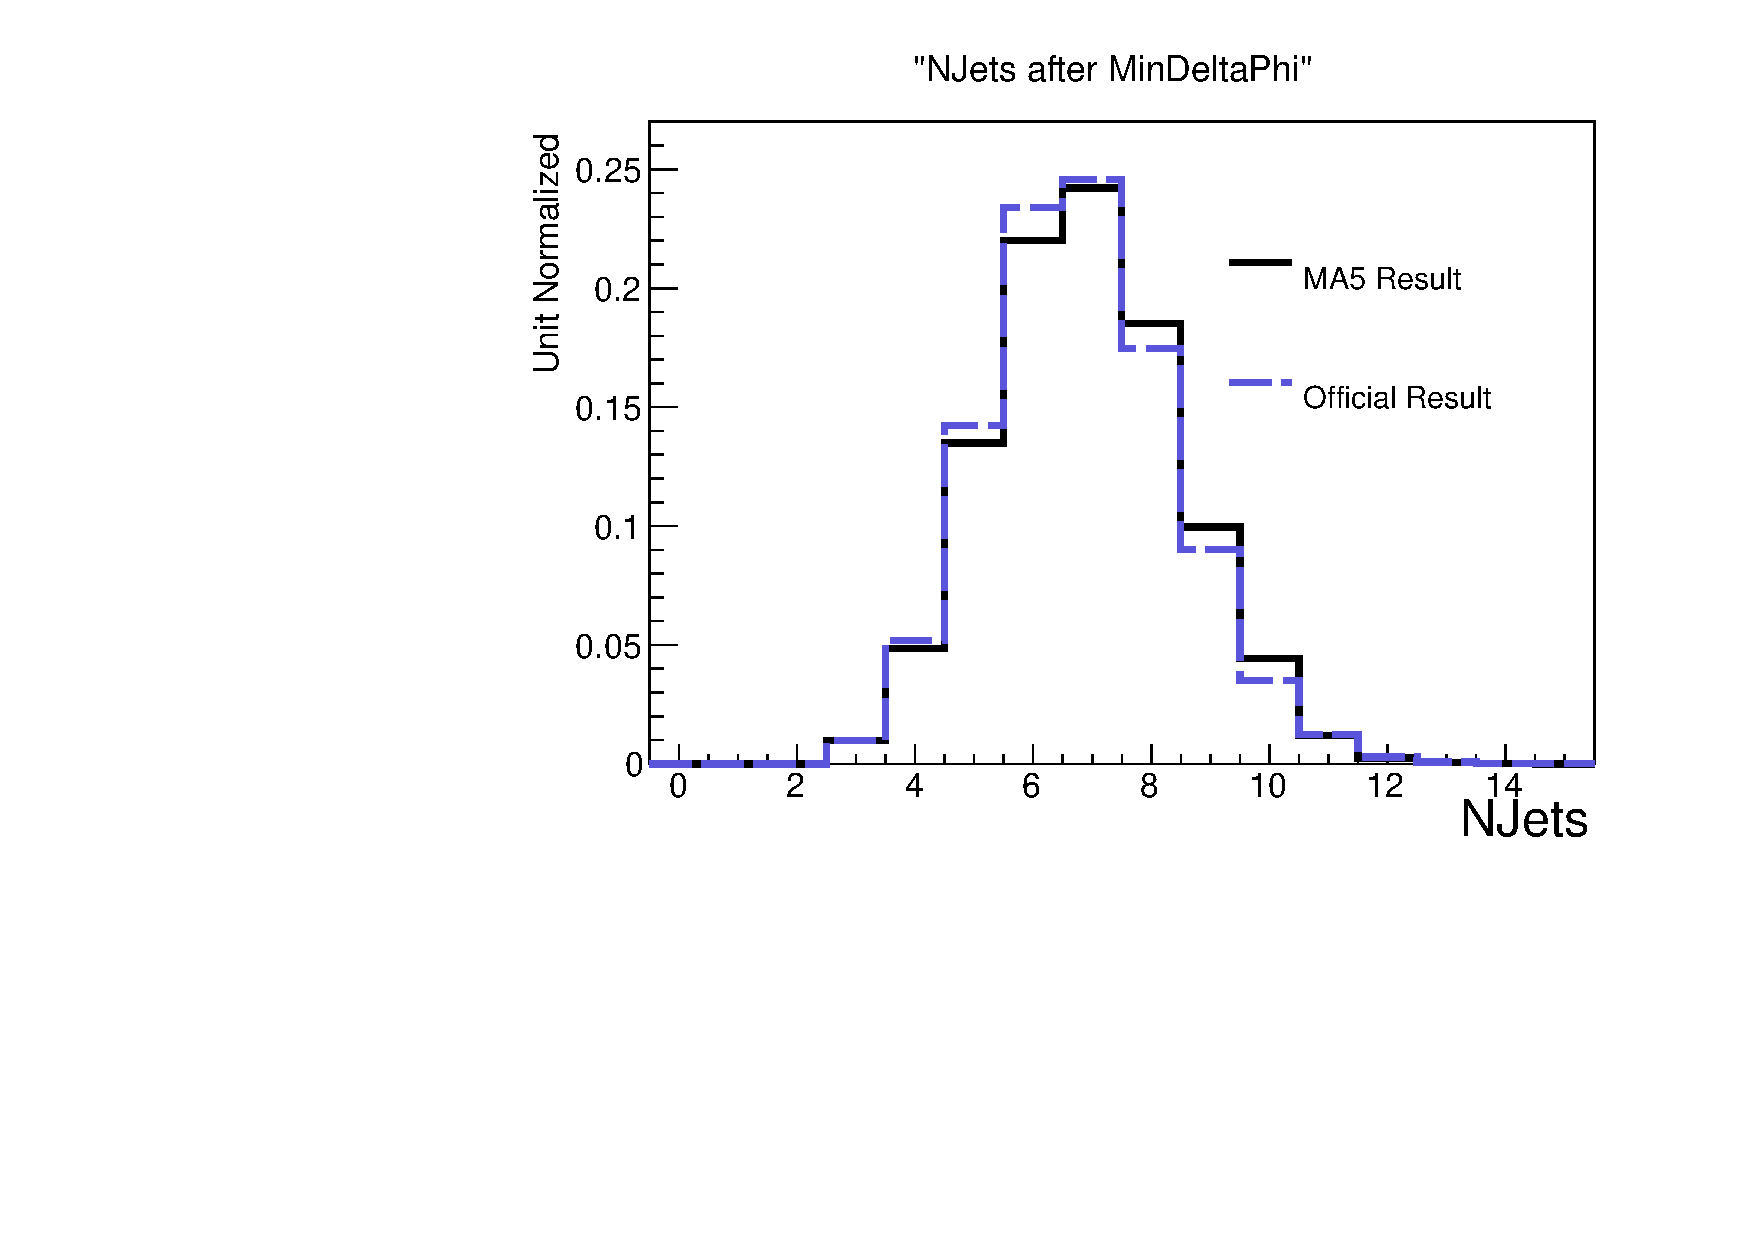
\includegraphics[width=0.5\textwidth]{figures/Appendices/Ma5ValidationSUS13012/T1tttt_NJets_after_MinDeltaPhi.pdf}
                \label{fig:tiger}
        }
        \caption{Comparison of the distributions of NJets between the official and our own samples after the ``n-1" cut, Min $\Delta(\phi)$ (left), and after all baseline cuts (right), for the T1tttt signal model.}\label{fig:animals}
\end{figure}        
        
        \begin{figure}
        \centering
        \subfloat[]{
        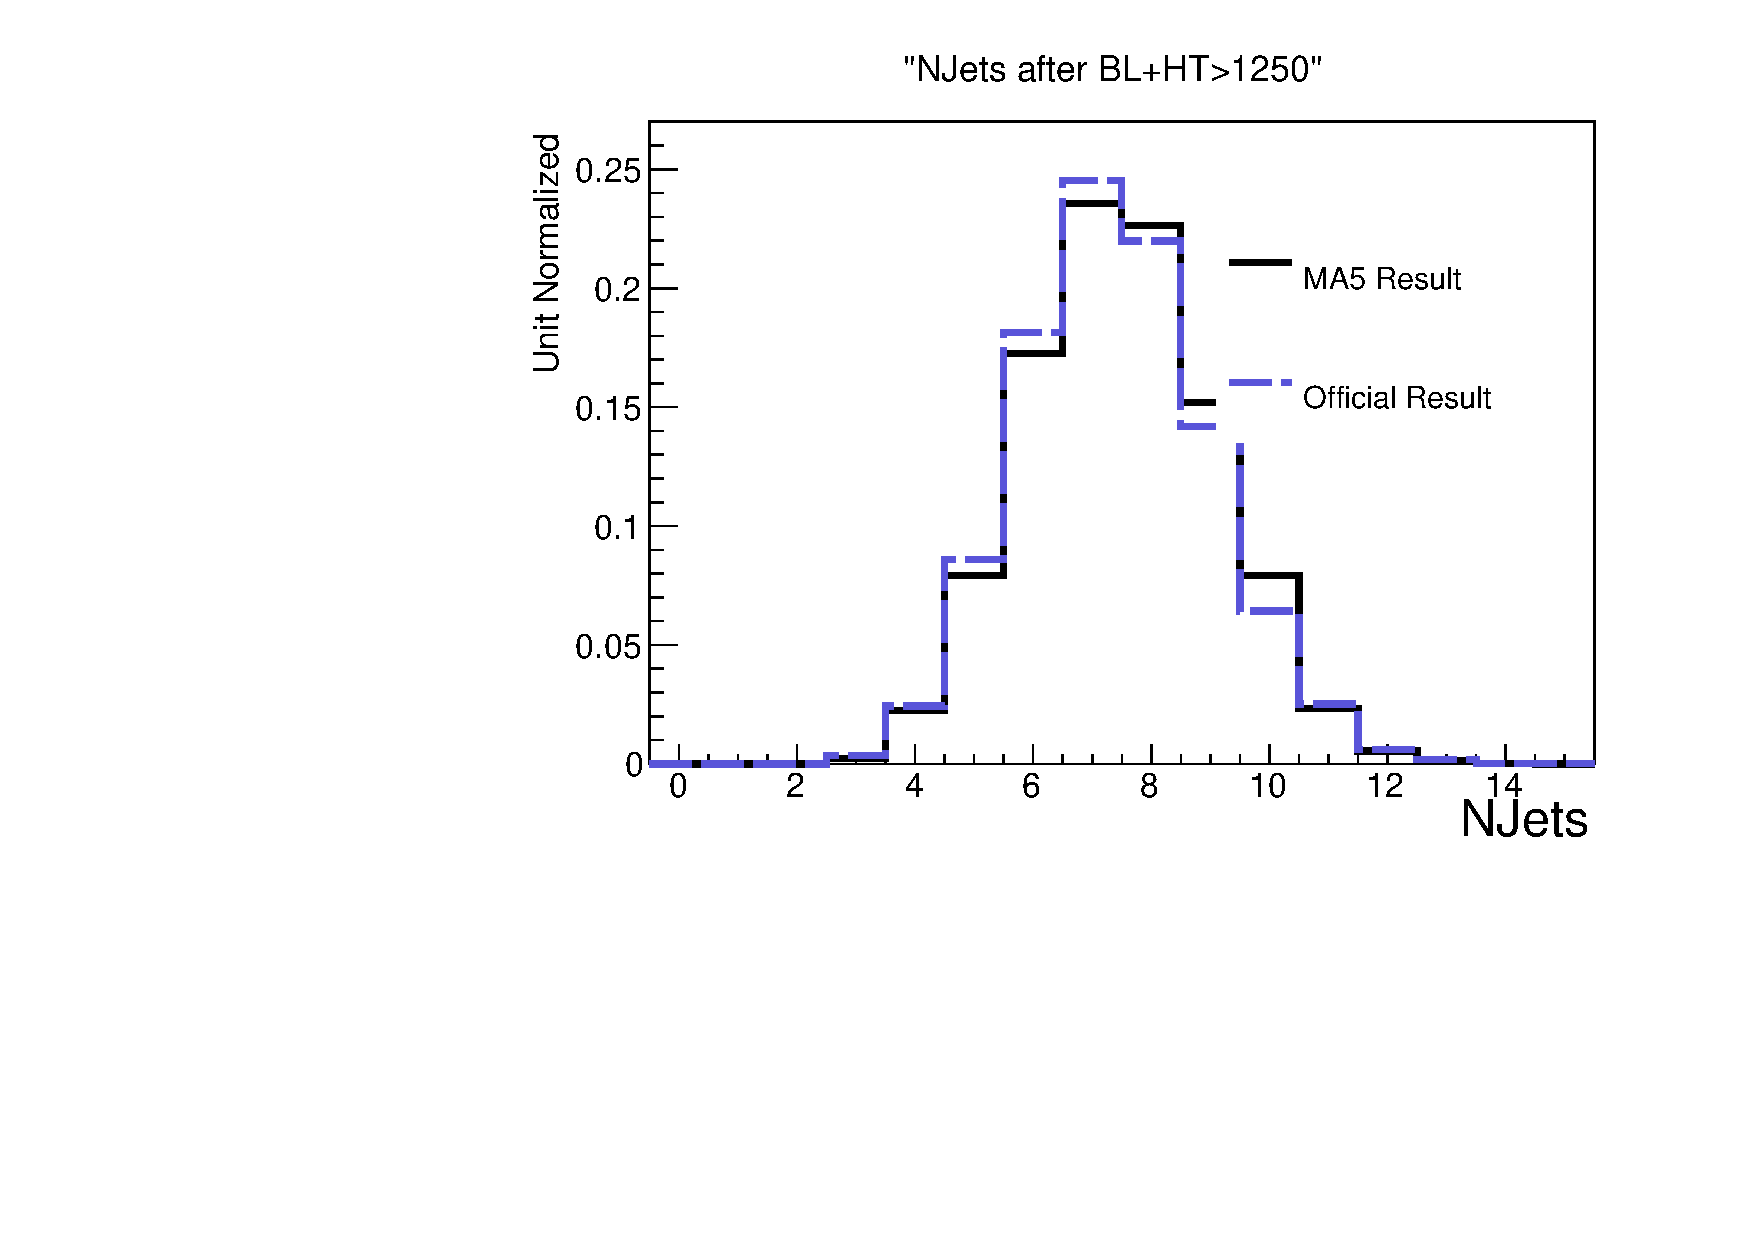
\includegraphics[width=0.5\textwidth]{figures/Appendices/Ma5ValidationSUS13012/T1tttt_NJets_after_BL+HT>1250.pdf}
        \label{fig:gull}
        }%
        \hspace{-1 cm}
        ~ %add desired spacing between images, e. g. ~, \quad, \qquad, \hfill etc.
        %(or a blank line to force the subfigure onto a new line)
        \subfloat[]{
        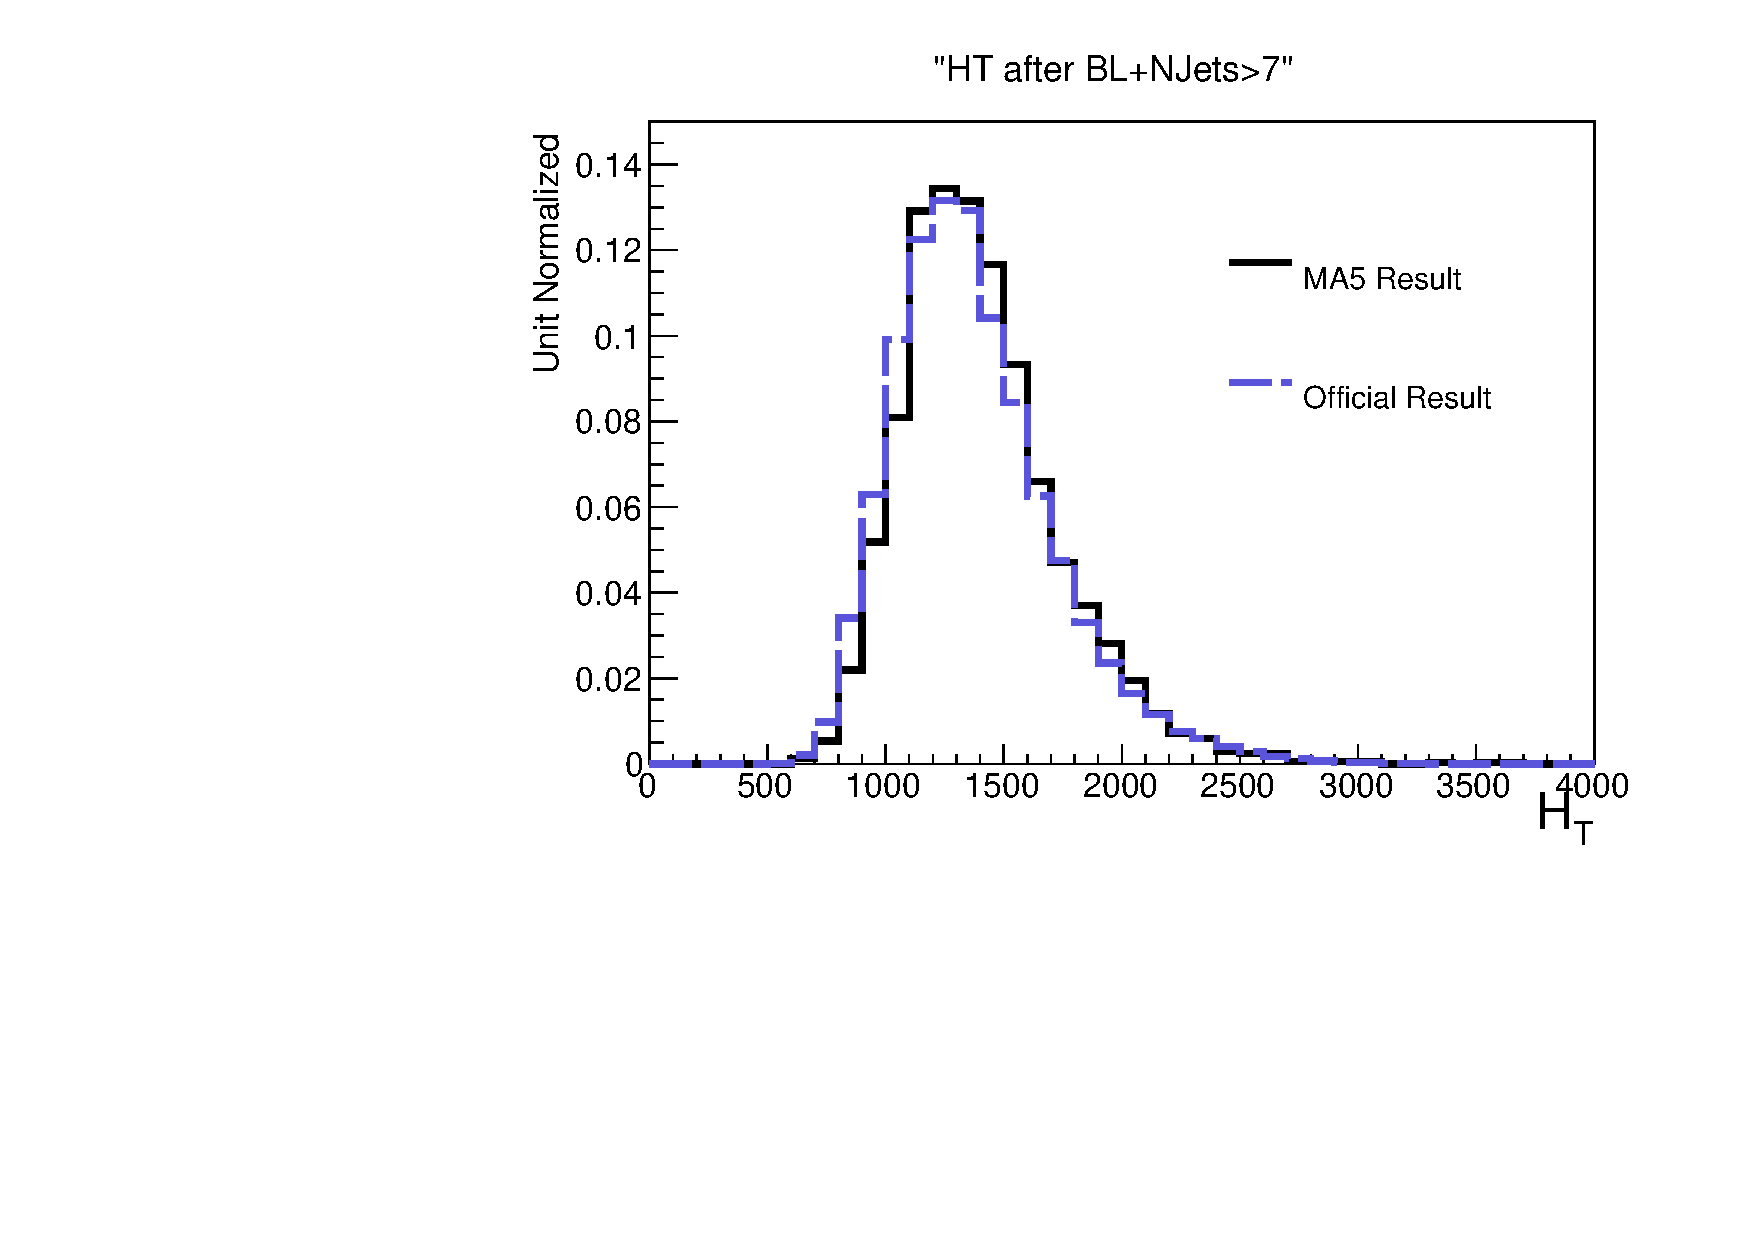
\includegraphics[width=0.5\textwidth]{figures/Appendices/Ma5ValidationSUS13012/T1tttt_HT_after_BL+NJets>7.pdf}
        \label{fig:tiger}
        }
        \caption{Additional checks: comparison between ours and the official distributions of NJets after BL+$H_T$$>$1250 cuts (left), and $H_T$ after BL+NJets$>$7 cuts (right), for the T1tttt signal model.}
        \end{figure}  
        

\clearpage
%%%%%%%%%%%%%%%%%%%%%%%%%%%%%%%%%%%%%%%%%%%%%%%%%
\subsubsection{T5VV simplified model}
%%%%%%%%%%%%%%%%%%%%%%%%%%%%%%%%%%%%%%%%%%%%%%%%%

\begin{figure}[h!]
\centering
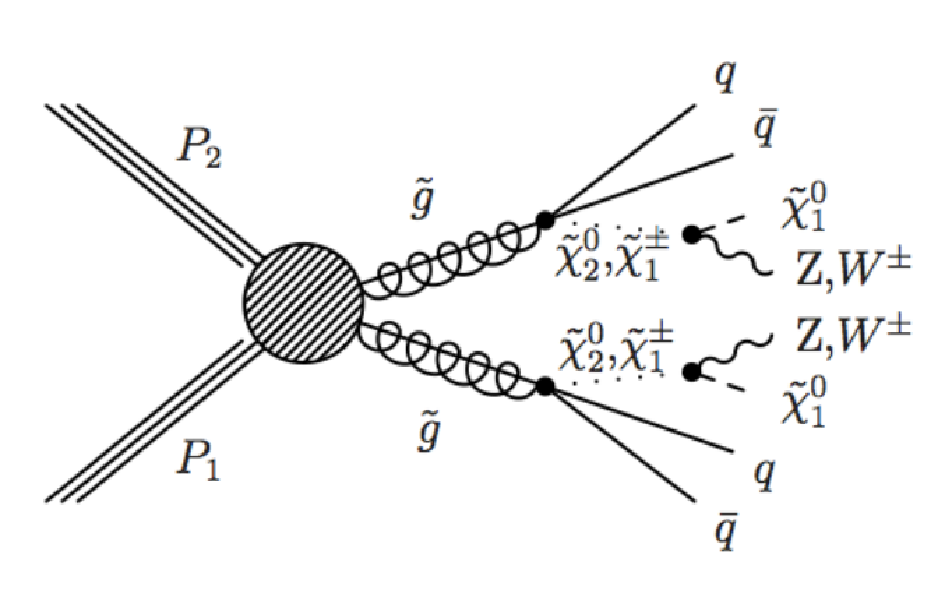
\includegraphics[width=7cm]{figures/Appendices/Ma5ValidationSUS13012/T5VV.pdf}
\caption{Diagram of the dominant SUSY production mechanism
for the T5VV signal model.}
\label{fig:T5VV}
\end{figure}

    \begin{table}[h!]
    \begin{centering}
    \begin{tabular}{  c | c | c  }
    \hline
    \hline
    Cut Name & Official Count (Eff) & MA5 Count (Eff)\\
    \hline
        MET Cleaning & 189.9 (xxx) & 189.9 (xxx)\\
    No Lepton & 136.2 (71\%) & 142.07 (74\%)\\
    NJets$>$2 & 135.9 (99\%) & 141.69 (99\%)\\
    $H_T$$>$500 & 135.5 (99\%) & 141.26 (99\%)\\
    \MHT$>$200 & 108.8 (80\%) & 115.23 (81\%)\\
    Min $\Delta(\phi)$ & 89.6 (82\%) & 95.22 (82\%)\\
\hline
\hline
    \end{tabular}
    \caption{The cut flow for the baseline selection in CMS SUS-13-012 for
    the T5VV working point $(m_{\tilde g},\,m_{\tilde\chi^0_1})=(1100,\,125)$~GeV.  
    The second column is the official account
    and our own results are given in column 3. The official counts are
    normalized to luminosity ${\cal L}=19.5$/fb and cross section $\sigma= 10.17$~pb, and our
    counts are normalized to match the official count after the first cut, MET
    Cleaning.}
    \label{table:CF3}
    \end{centering}
    \end{table}
    
    \begin{table}
    \begin{centering}
    \begin{tabular}{  l | c | c  }
    \hline
    \hline
    Signal Region Name & Official & MA5\\
    \hline
    NJets3-5,  $H_T$500-800,  \MHT200-300 & 1.0 & 1.18\\ 
 \hline 
NJets3-5,  $H_T$500-800,  \MHT300-450 & 1.8 & 1.77\\ 
 \hline 
NJets3-5,  $H_T$500-800,  \MHT450-600 & 1.1 & 1.09\\ 
 \hline 
NJets3-5,  $H_T$500-800,  \MHT$>$600 & 0.3 & 0.31\\ 
 \hline 
NJets3-5,  $H_T$800-1000,  \MHT200-300 & 1.5 & 1.08\\ 
 \hline 
NJets3-5,  $H_T$800-1000,  \MHT300-450 & 1.7 & 2.40\\ 
 \hline 
NJets3-5,  $H_T$800-1000,  \MHT450-600 & 2.1 & 2.12\\ 
 \hline 
NJets3-5,  $H_T$800-1000,  \MHT$>$600 & 1.2 & 1.43\\ 
 \hline 
NJets3-5,  $H_T$1000-1250,  \MHT200-300 & 1.9 & 1.84\\ 
 \hline 
NJets3-5,  $H_T$1000-1250,  \MHT300-450 & 3.1 & 3.23\\ 
 \hline 
NJets3-5,  $H_T$1000-1250,  \MHT450-600 & 2.8 & 2.66\\ 
 \hline 
NJets3-5,  $H_T$1000-1250,  \MHT$>$600 & 2.1 & 2.41\\ 
 \hline 
NJets3-5,  $H_T$1250-1500,  \MHT200-300 & 1.3 & 1.35\\ 
 \hline 
NJets3-5,  $H_T$1250-1500,  \MHT300-450 & 2.3 & 2.03\\ 
 \hline 
NJets3-5,  $H_T$1250-1500,  \MHT$>$450 & 3.2 & 3.67\\ 
 \hline 
NJets3-5,  $H_T$$>$1500,  \MHT200-300 & 1.1 & 1.06\\ 
 \hline 
NJets3-5,  $H_T$$>$1500,  \MHT$>$300 & 3.7 & 3.77\\ 
 \hline 
NJets6-7,  $H_T$500-800,  \MHT200-300 & 0.4 & 0.29\\ 
 \hline 
NJets6-7,  $H_T$500-800,  \MHT300-450 & 0.4 & 0.32\\ 
 \hline 
NJets6-7,  $H_T$500-800,  \MHT$>$450 & 0.2 & 0.15\\ 
 \hline 
NJets6-7,  $H_T$800-1000,  \MHT200-300 & 1.2 & 1.06\\ 
 \hline 
NJets6-7,  $H_T$800-1000,  \MHT300-450 & 1.9 & 1.73\\ 
 \hline 
NJets6-7,  $H_T$800-1000,  \MHT$>$450 & 1.7 & 1.65\\ 
 \hline 
NJets6-7,  $H_T$1000-1250,  \MHT200-300 & 3.1 & 2.66\\ 
 \hline 
NJets6-7,  $H_T$1000-1250,  \MHT300-450 & 4.6 & 4.72\\ 
 \hline 
NJets6-7,  $H_T$1000-1250,  \MHT$>$450 & 5.9 & 5.77\\ 
 \hline 
NJets6-7,  $H_T$1250-1500,  \MHT200-300 & 2.7 & 2.89\\ 
 \hline 
NJets6-7,  $H_T$1250-1500,  \MHT300-450 & 4.4 & 4.72\\ 
 \hline 
NJets6-7,  $H_T$1250-1500,  \MHT$>$450 & 5.8 & 6.57\\ 
 \hline 
NJets6-7,  $H_T$$>$1500,  \MHT200-300 & 2.7 & 3.01\\ 
 \hline 
NJets6-7,  $H_T$$>$1500,  \MHT$>$300 & 9.2 & 10.94\\ 
 \hline 
NJets$>$7,  $H_T$500-800,  \MHT$>$200 & 0.0 & 0.01\\ 
 \hline 
NJets$>$7,  $H_T$800-1000,  \MHT$>$200 & 0.4 & 0.33\\ 
 \hline 
NJets$>$7,  $H_T$1000-1250,  \MHT$>$200 & 2.3 & 2.50\\ 
 \hline 
NJets$>$7,  $H_T$1250-1500,  \MHT$>$200 & 3.8 & 4.48\\ 
 \hline 
NJets$>$7,  $H_T$$>$1500,  \MHT$>$200 & 6.0 & 7.84\\ 
 \hline 
\hline
    \end{tabular}
    \caption{The signal region (SR) counts in CMS SUS-13-012 for the T5VV scenario 
     after all selection has been applied. Column 2 is the official account obtained through generous correspondence with Christian Sanders,
    and our own results displayed in column 3. These counts were determined by applying the SR selection to the end of the cut flow featured in table \ref{table:CF3}.}
    \end{centering}
    \end{table}
    
\begin{figure}
        \centering
        \subfloat[]{
                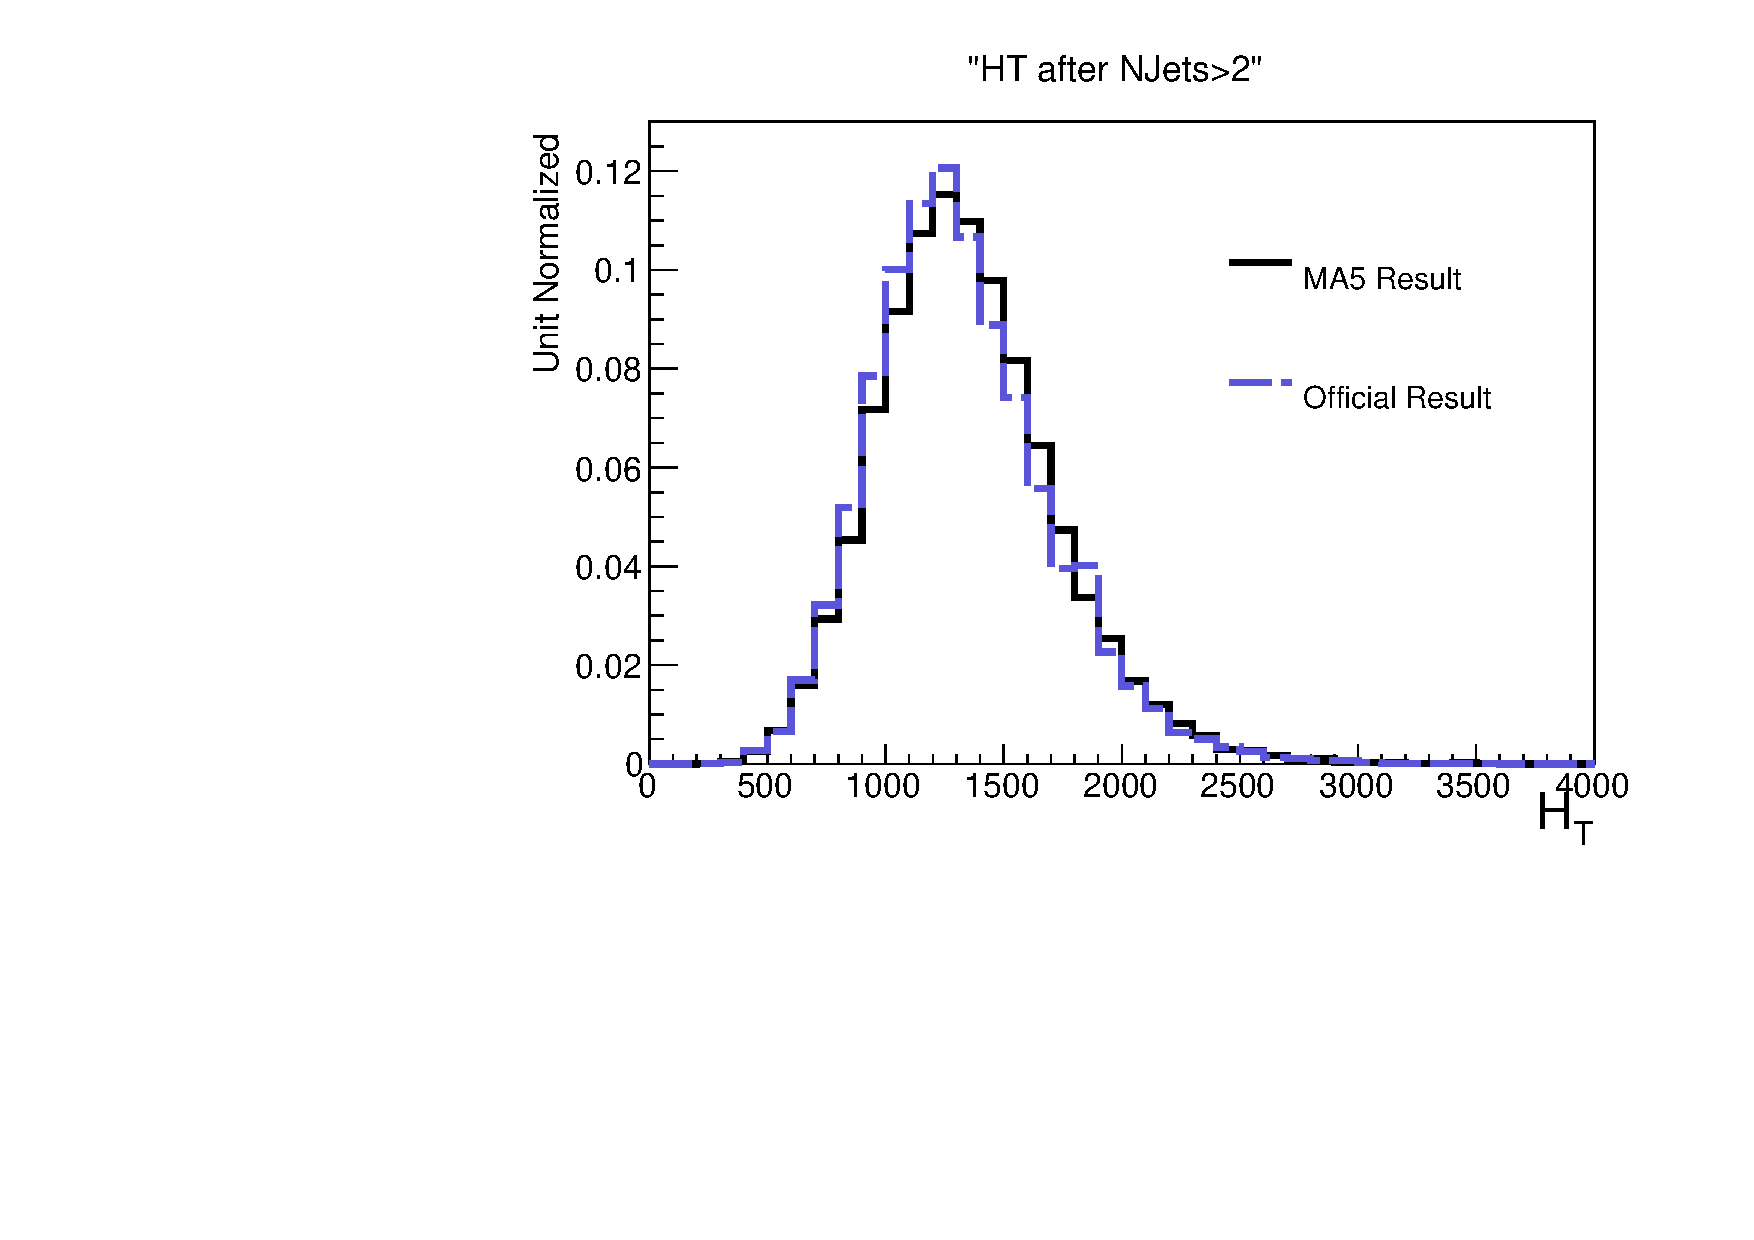
\includegraphics[width=0.5\textwidth]{figures/Appendices/Ma5ValidationSUS13012/T5VV_HT_after_NJets>2.pdf}
                \label{fig:gull}
        }%
        \hspace{-1 cm}
        ~ %add desired spacing between images, e. g. ~, \quad, \qquad, \hfill etc.
          %(or a blank line to force the subfigure onto a new line)
        \subfloat[]{
                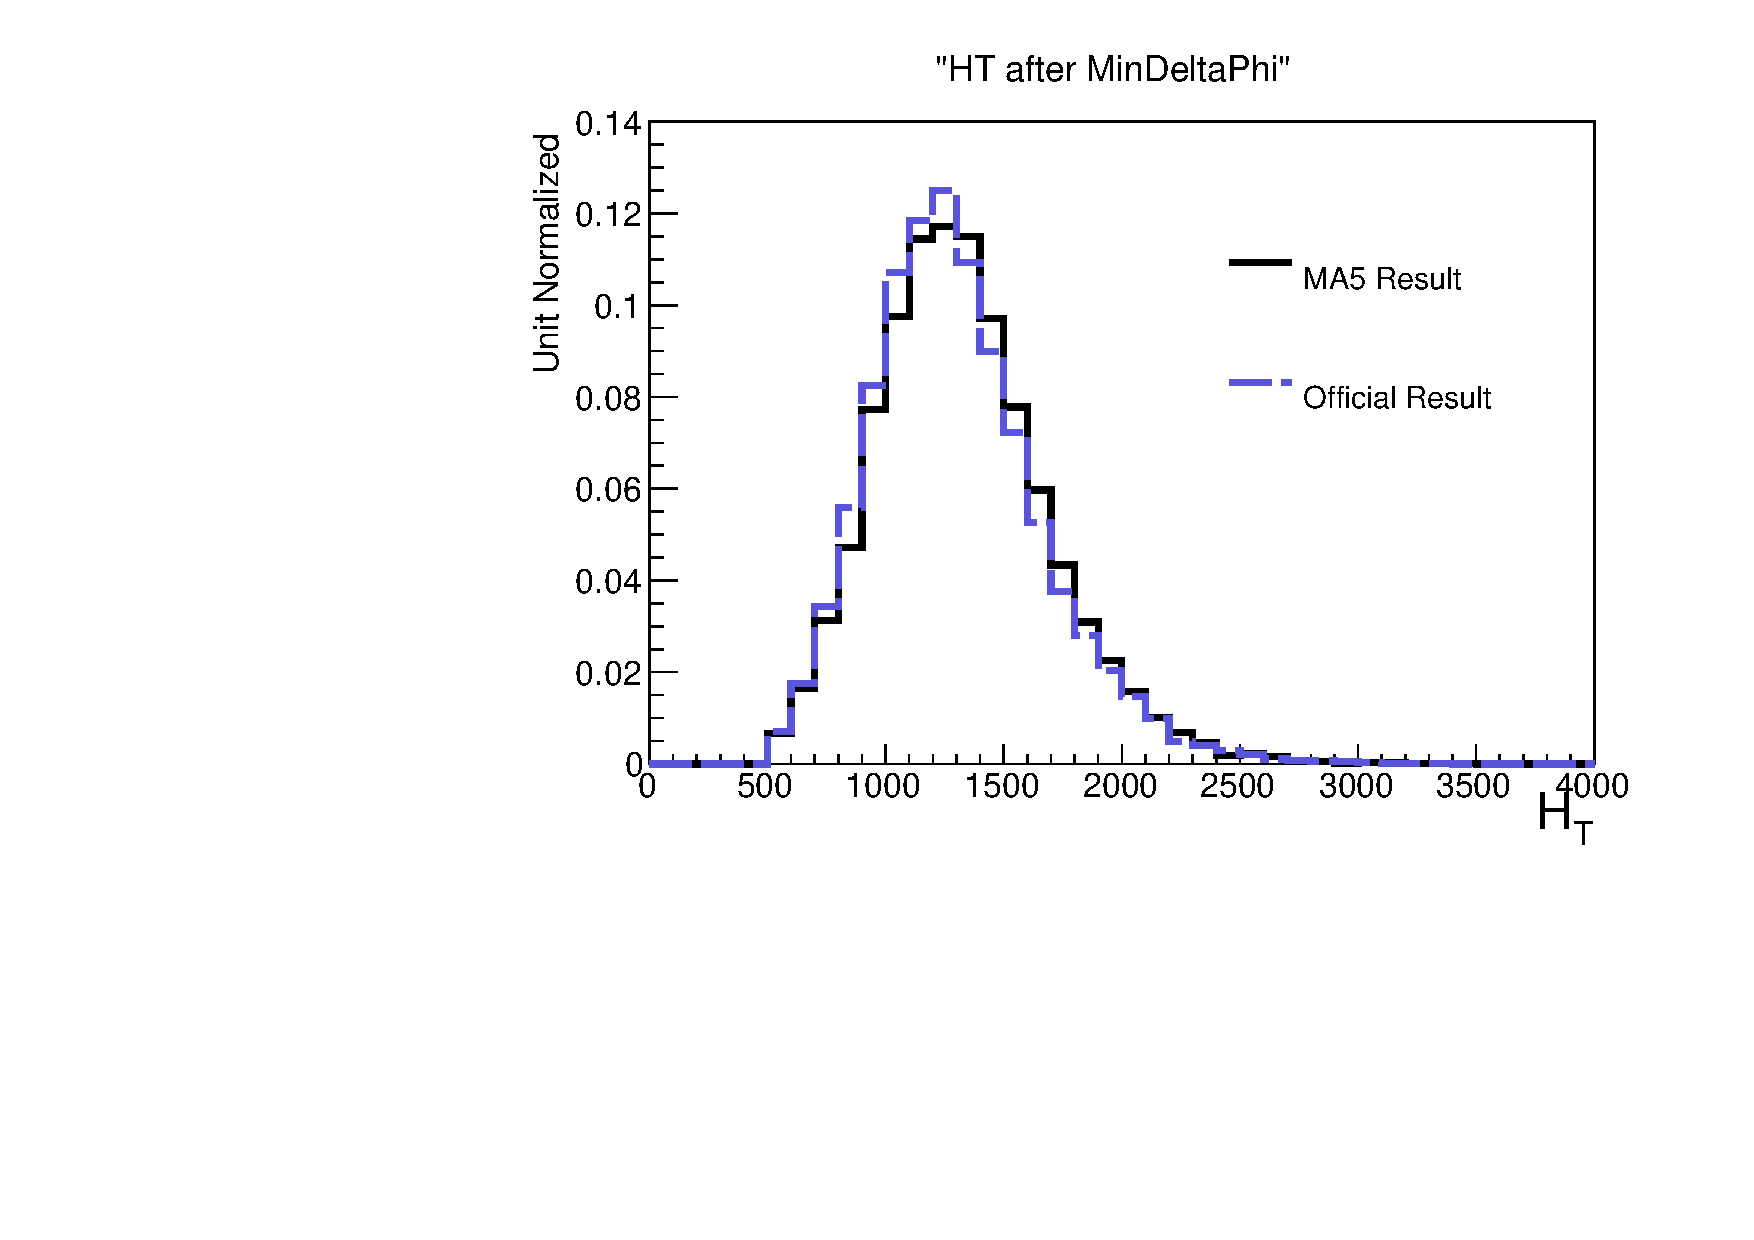
\includegraphics[width=0.5\textwidth]{figures/Appendices/Ma5ValidationSUS13012/T5VV_HT_after_MinDeltaPhi.pdf}
                \label{fig:tiger}
        }
        \caption{Comparison of the distributions of $H_T$ between the official and our own samples after the ``n-1" cut, Min $\Delta(\phi)$ (left), and after all baseline cuts (right), for the T5VV signal model.}\label{fig:animals}
\end{figure}        
        
\begin{figure}
        \centering
        \subfloat[]{
                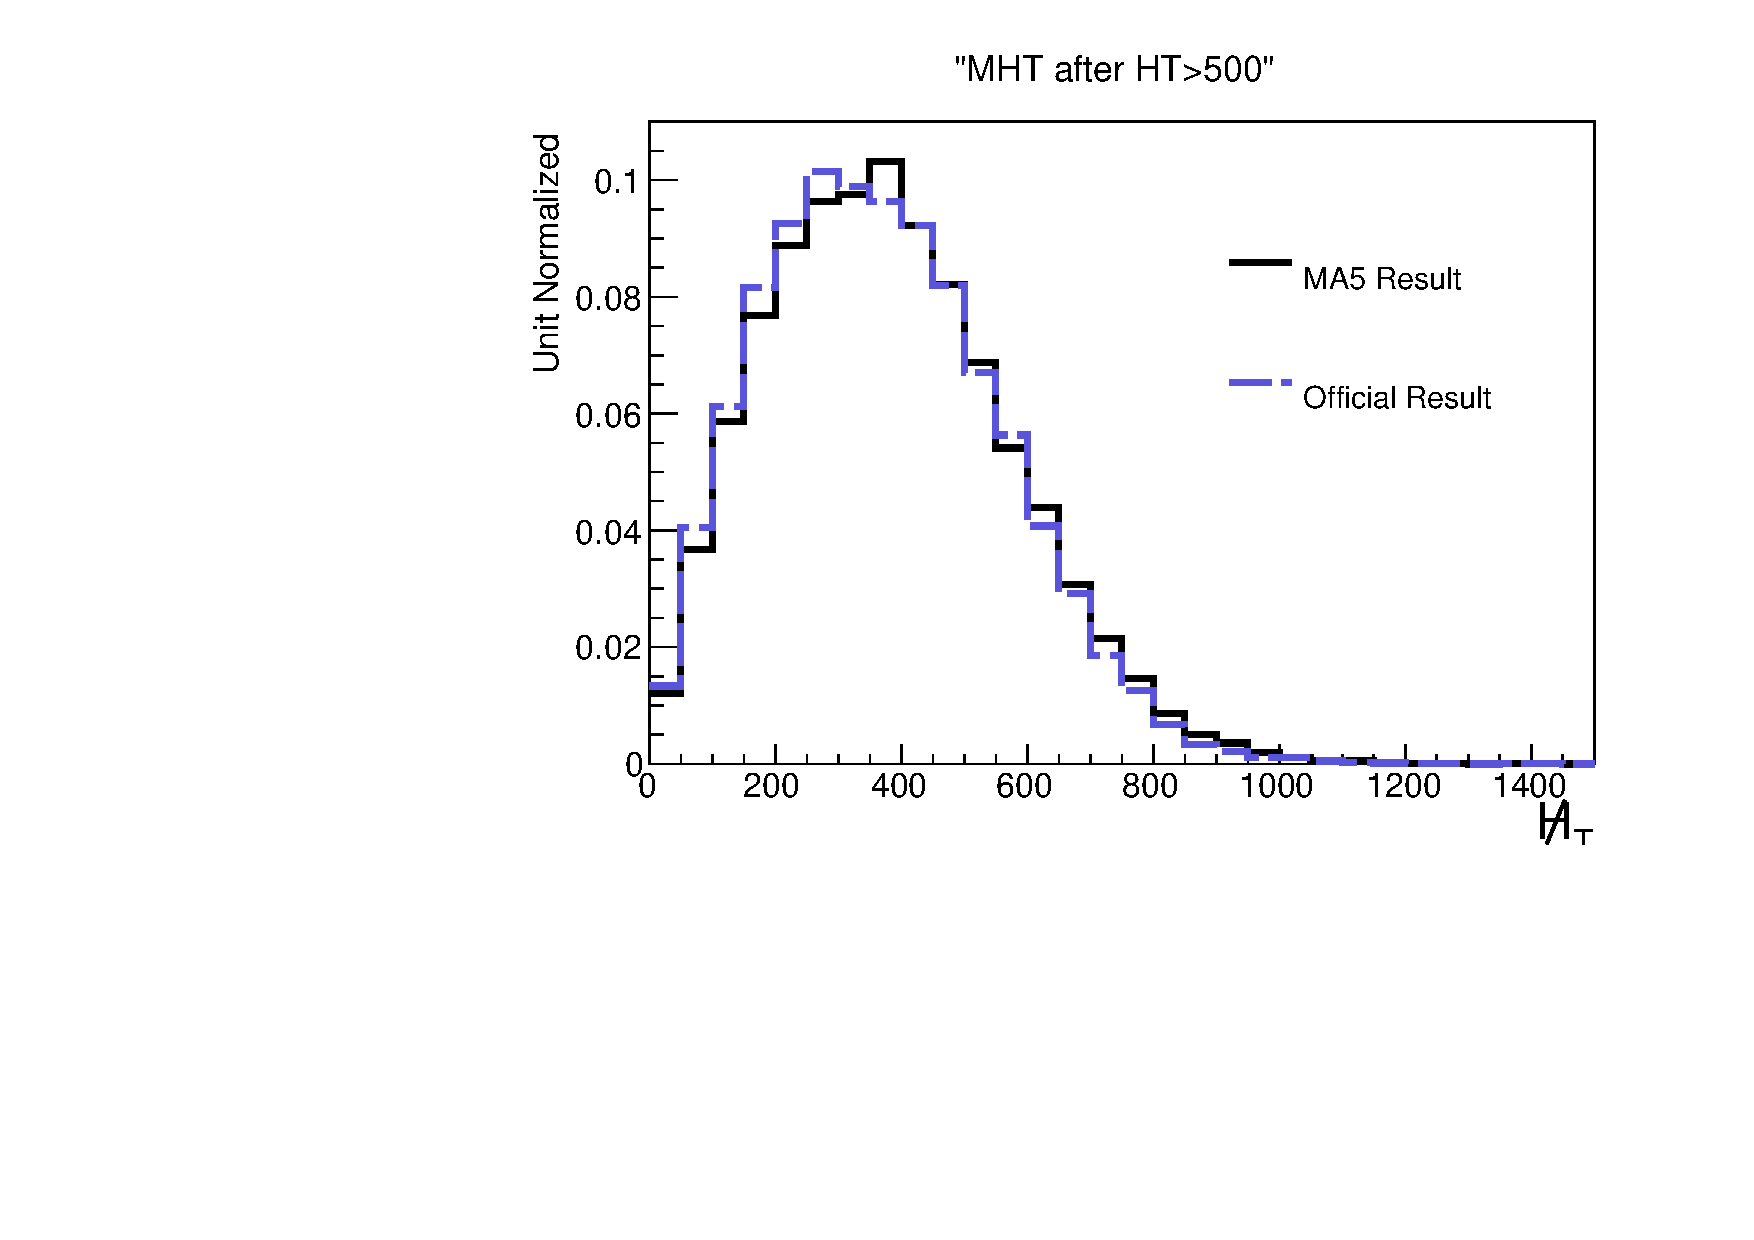
\includegraphics[width=0.5\textwidth]{figures/Appendices/Ma5ValidationSUS13012/T5VV_MHT_after_HT>500.pdf}
                \label{fig:gull}
        }%
        \hspace{-1 cm}
        ~ %add desired spacing between images, e. g. ~, \quad, \qquad, \hfill etc.
          %(or a blank line to force the subfigure onto a new line)
        \subfloat[]{
                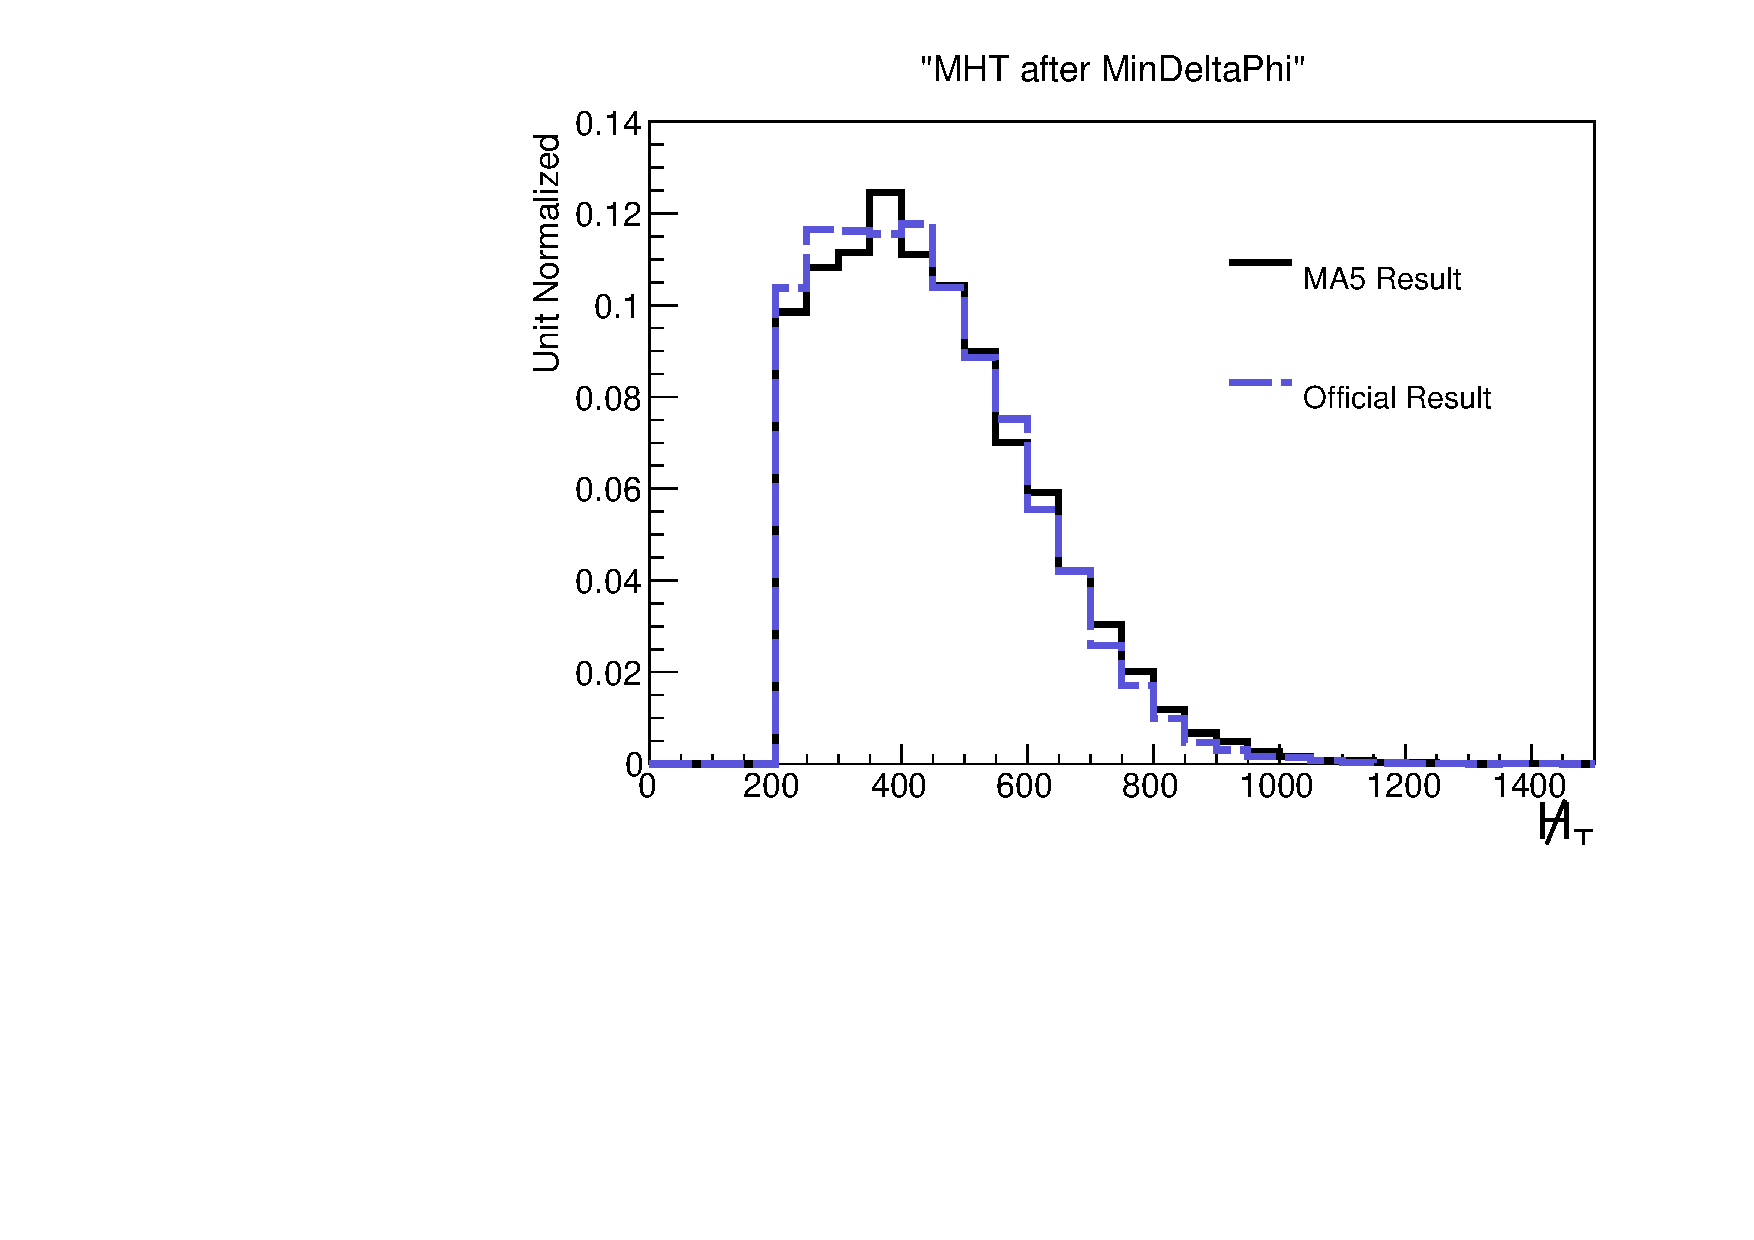
\includegraphics[width=0.5\textwidth]{figures/Appendices/Ma5ValidationSUS13012/T5VV_MHT_after_MinDeltaPhi.pdf}
                \label{fig:tiger}
        }
        \caption{Comparison of the distributions of \MHT between the official and our own samples after the ``n-1" cut, Min $\Delta(\phi)$ (left), and after all baseline cuts (right), for the T5VV signal model.}\label{fig:animals}
\end{figure}        
        
\begin{figure}
        \centering
        \subfloat[]{
                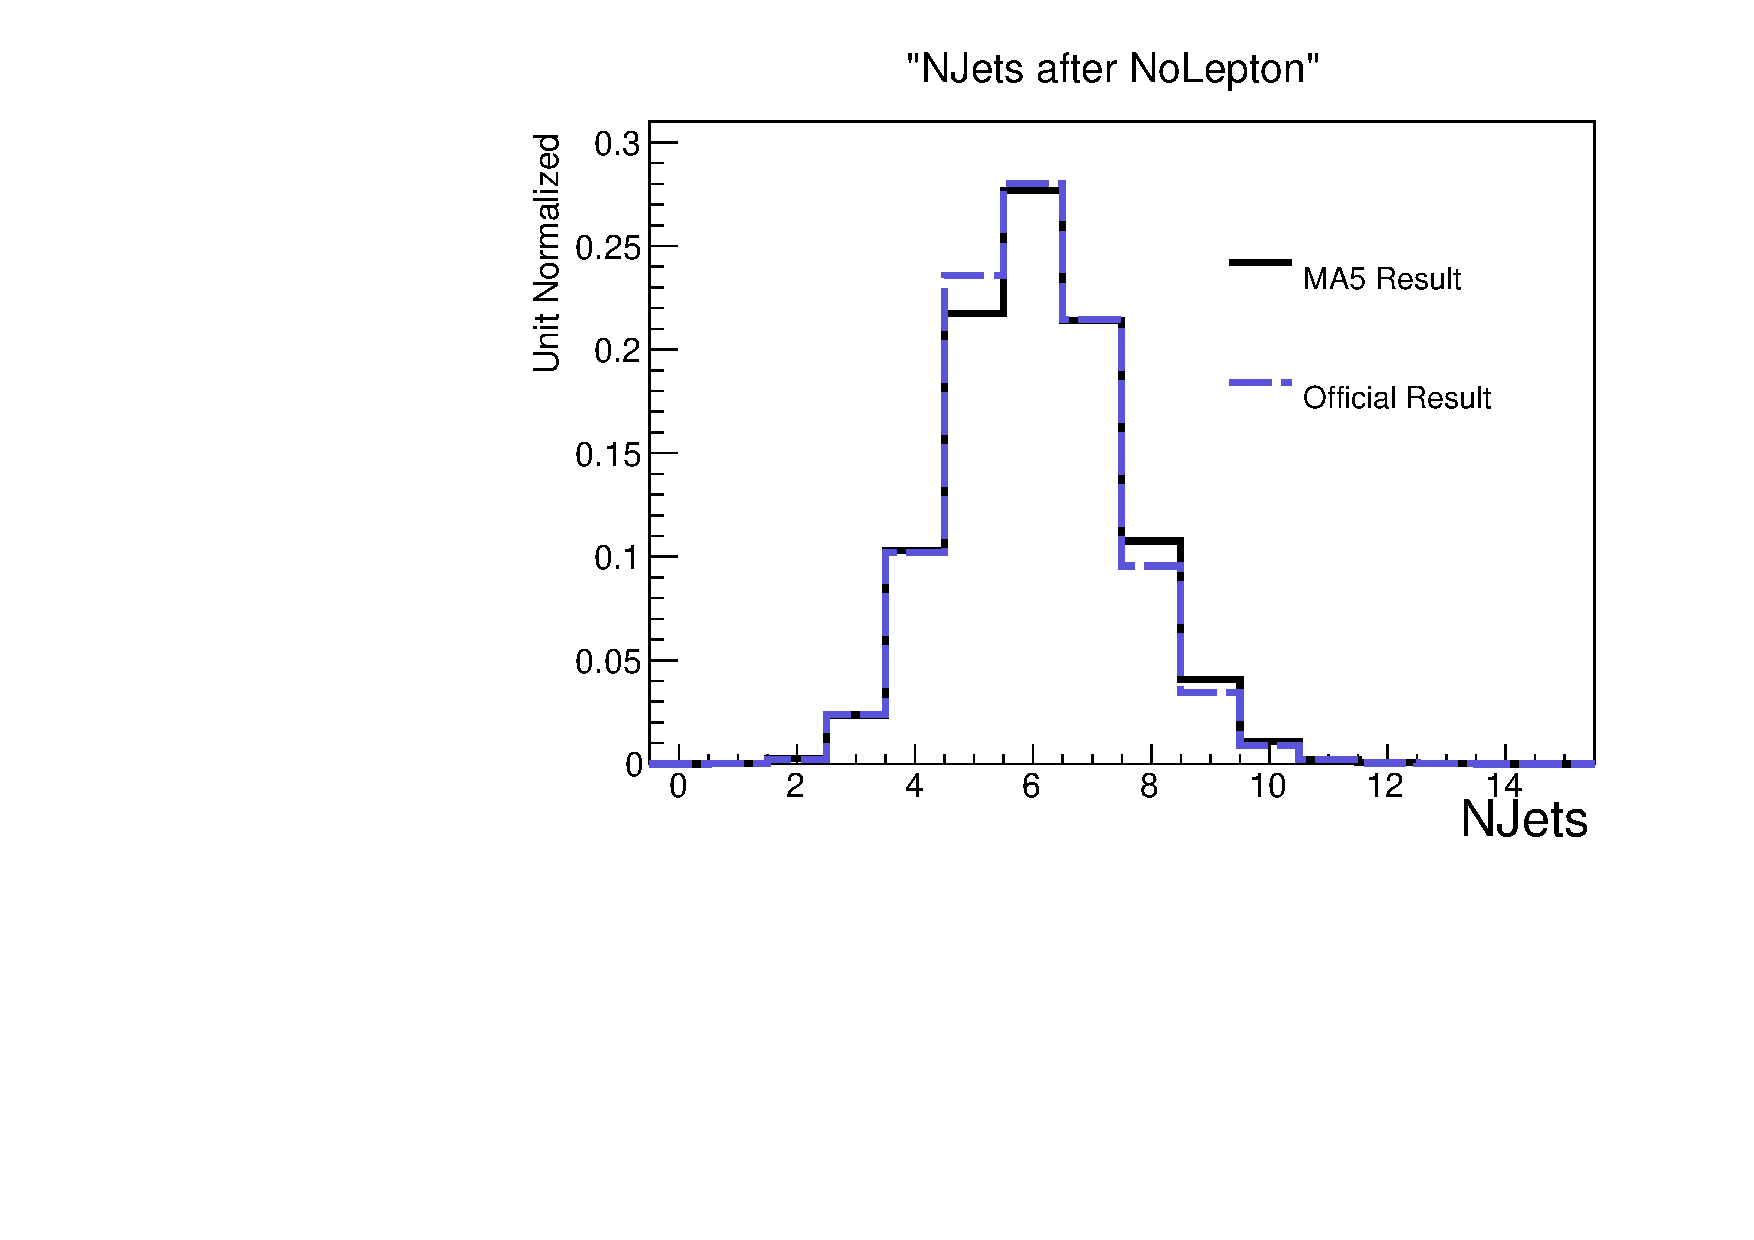
\includegraphics[width=0.5\textwidth]{figures/Appendices/Ma5ValidationSUS13012/T5VV_NJets_after_NoLepton.pdf}
                \label{fig:gull}
        }%
        \hspace{-1 cm}
        ~ %add desired spacing between images, e. g. ~, \quad, \qquad, \hfill etc.
          %(or a blank line to force the subfigure onto a new line)
        \subfloat[]{
                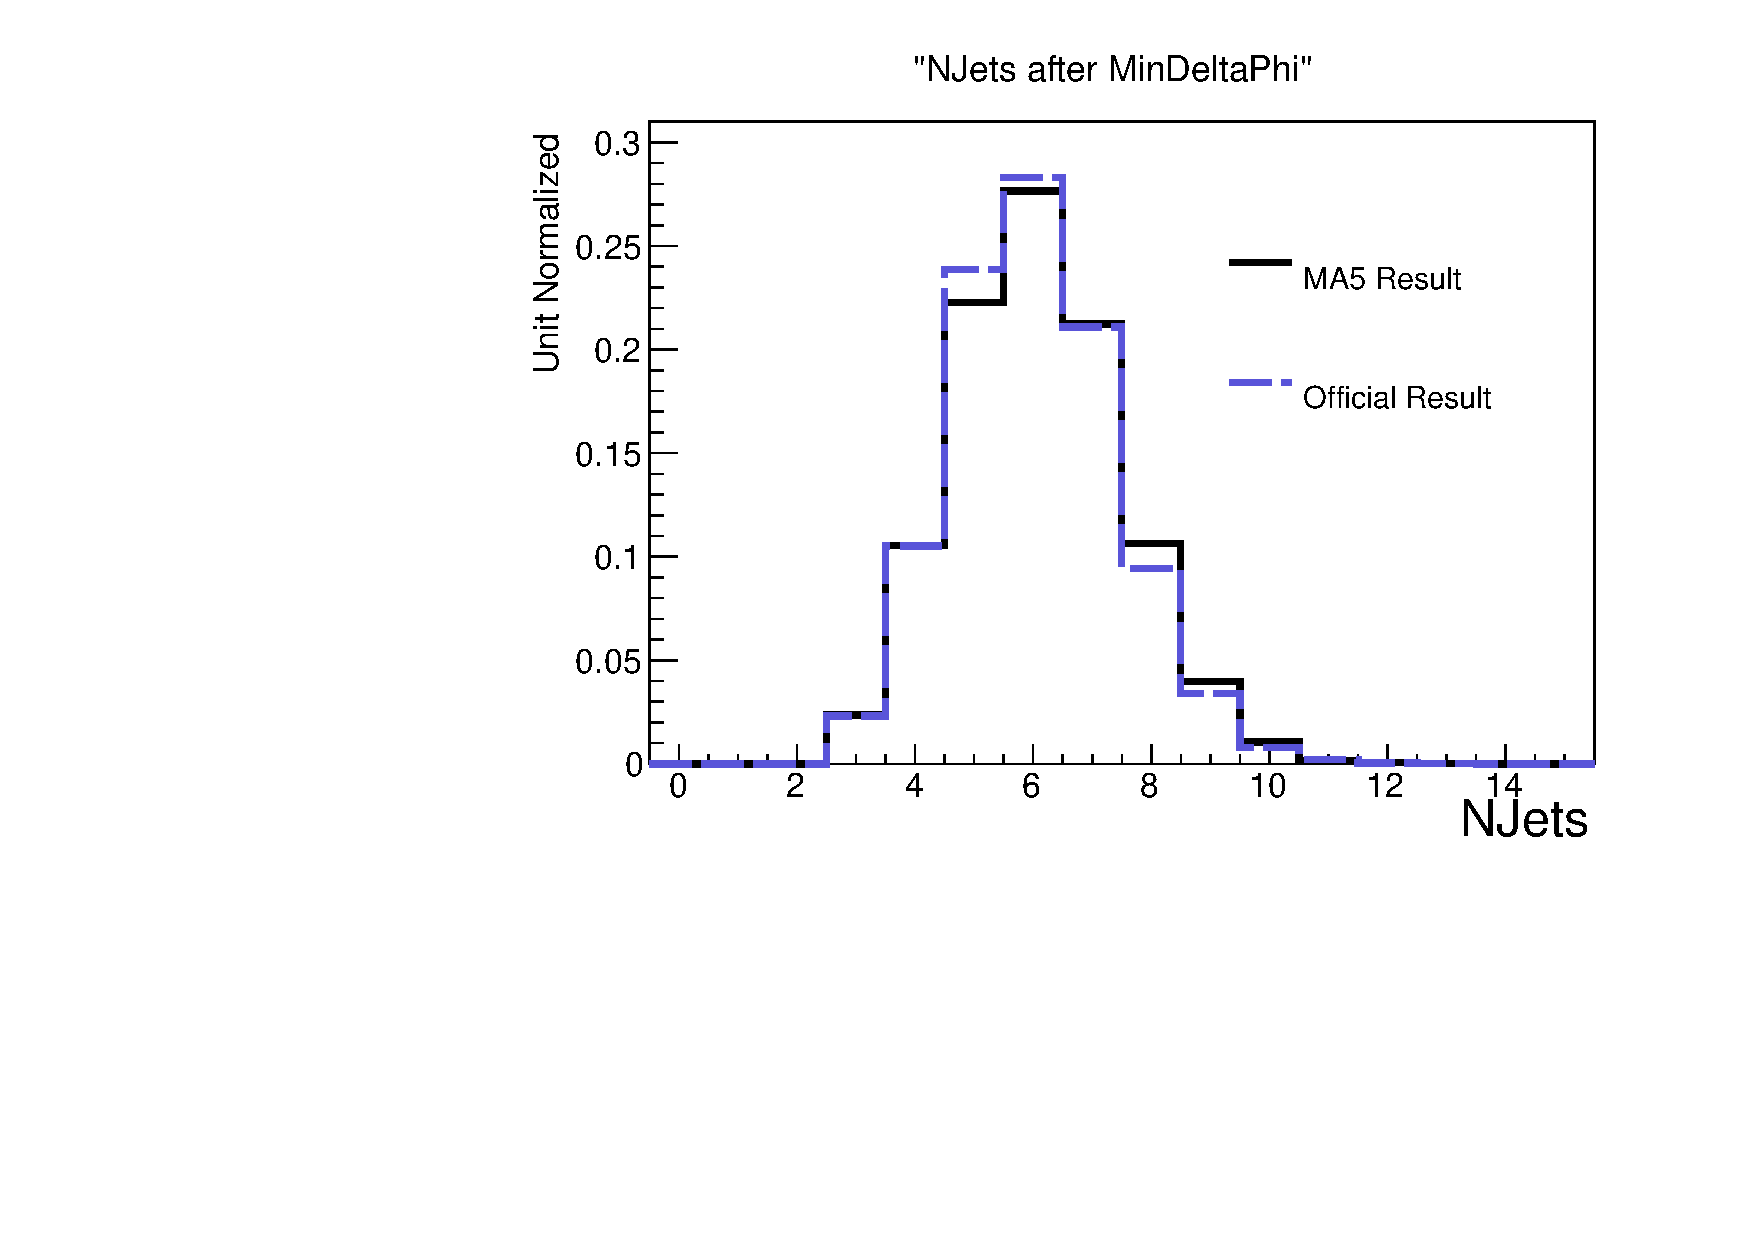
\includegraphics[width=0.5\textwidth]{figures/Appendices/Ma5ValidationSUS13012/T5VV_NJets_after_MinDeltaPhi.pdf}
                \label{fig:tiger}
        }
        \caption{Comparison of the distributions of NJets between the official and our own samples after the ``n-1" cut, Min $\Delta(\phi)$ (left), and after all baseline cuts (right), for the T5VV signal model.}\label{fig:animals}
\end{figure}        
        
        \begin{figure}
        \centering
        \subfloat[]{
        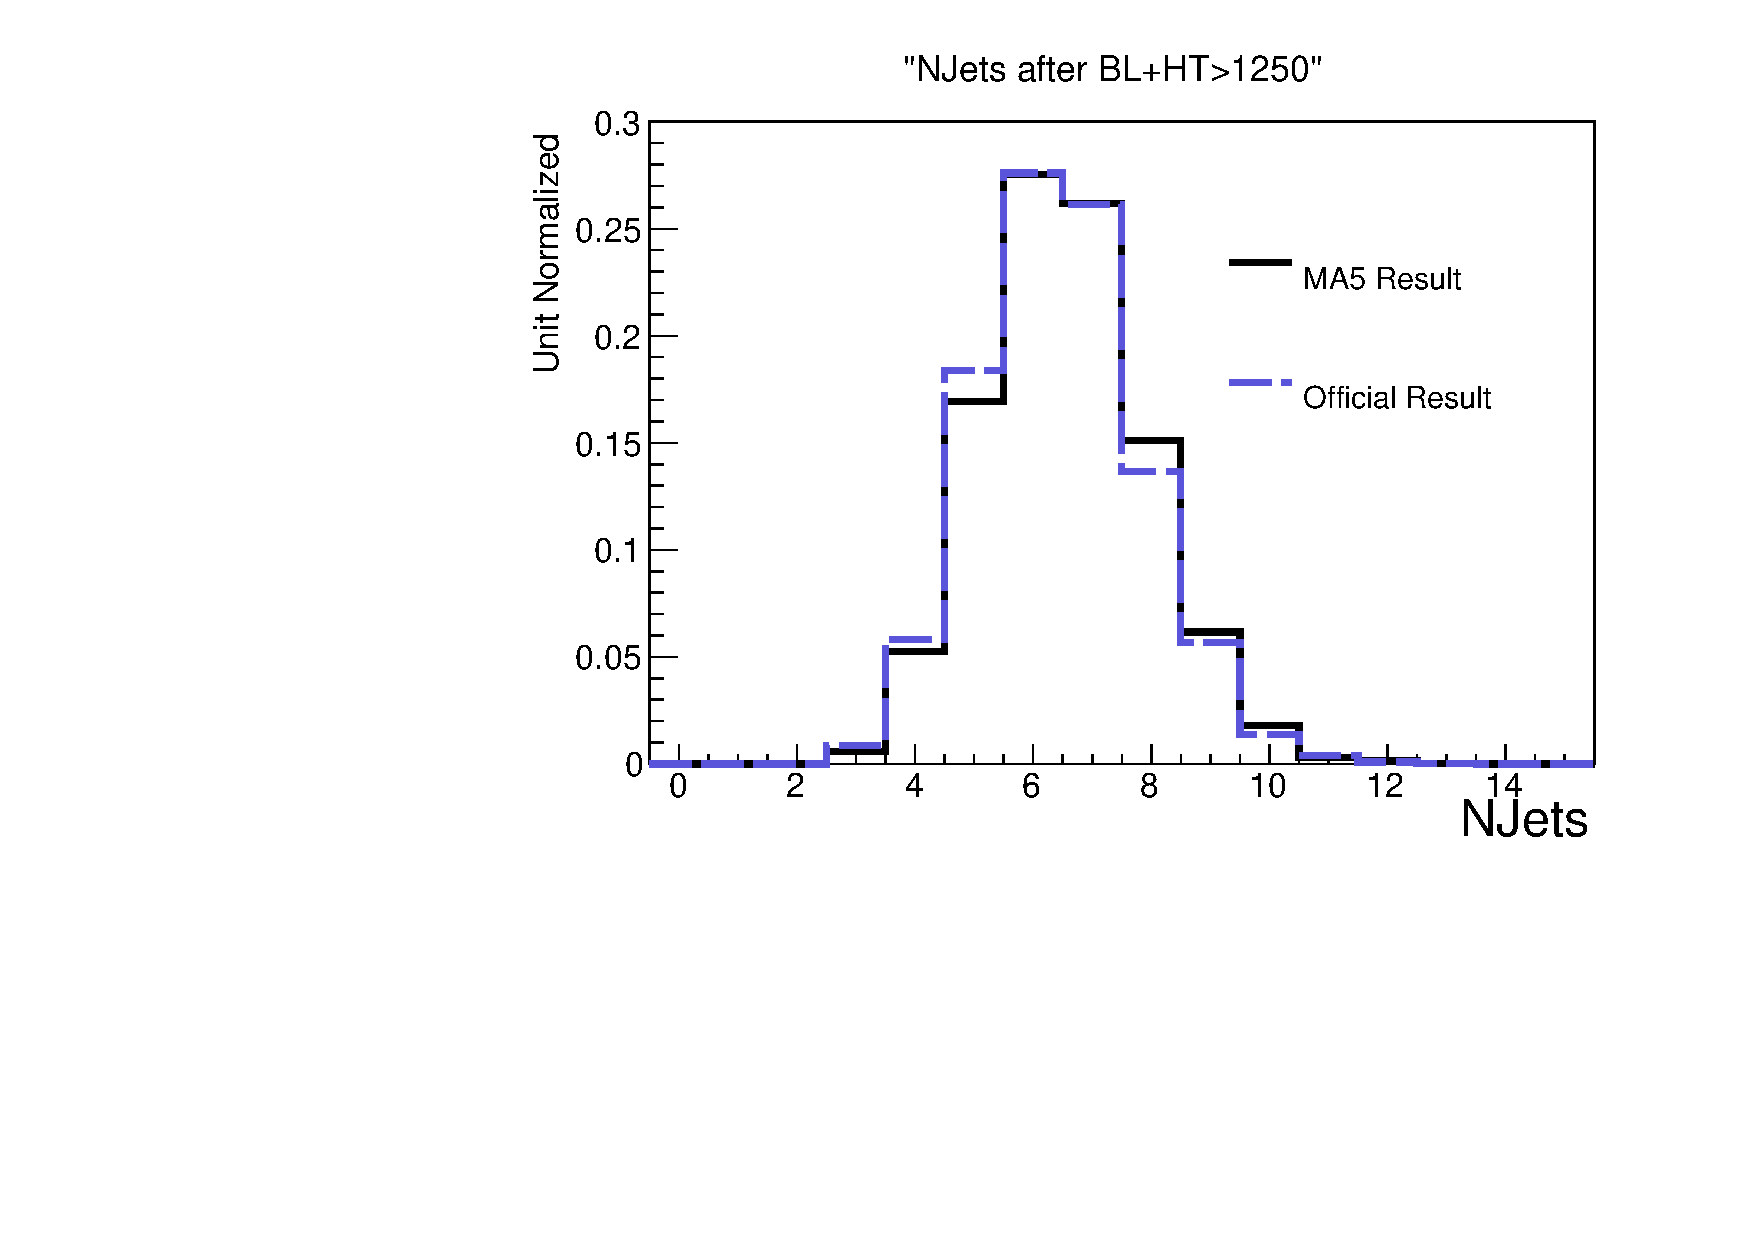
\includegraphics[width=0.5\textwidth]{figures/Appendices/Ma5ValidationSUS13012/T5VV_NJets_after_BL+HT>1250.pdf}
        \label{fig:gull}
        }%
        \hspace{-1 cm}
        ~ %add desired spacing between images, e. g. ~, \quad, \qquad, \hfill etc.
        %(or a blank line to force the subfigure onto a new line)
        \subfloat[]{
        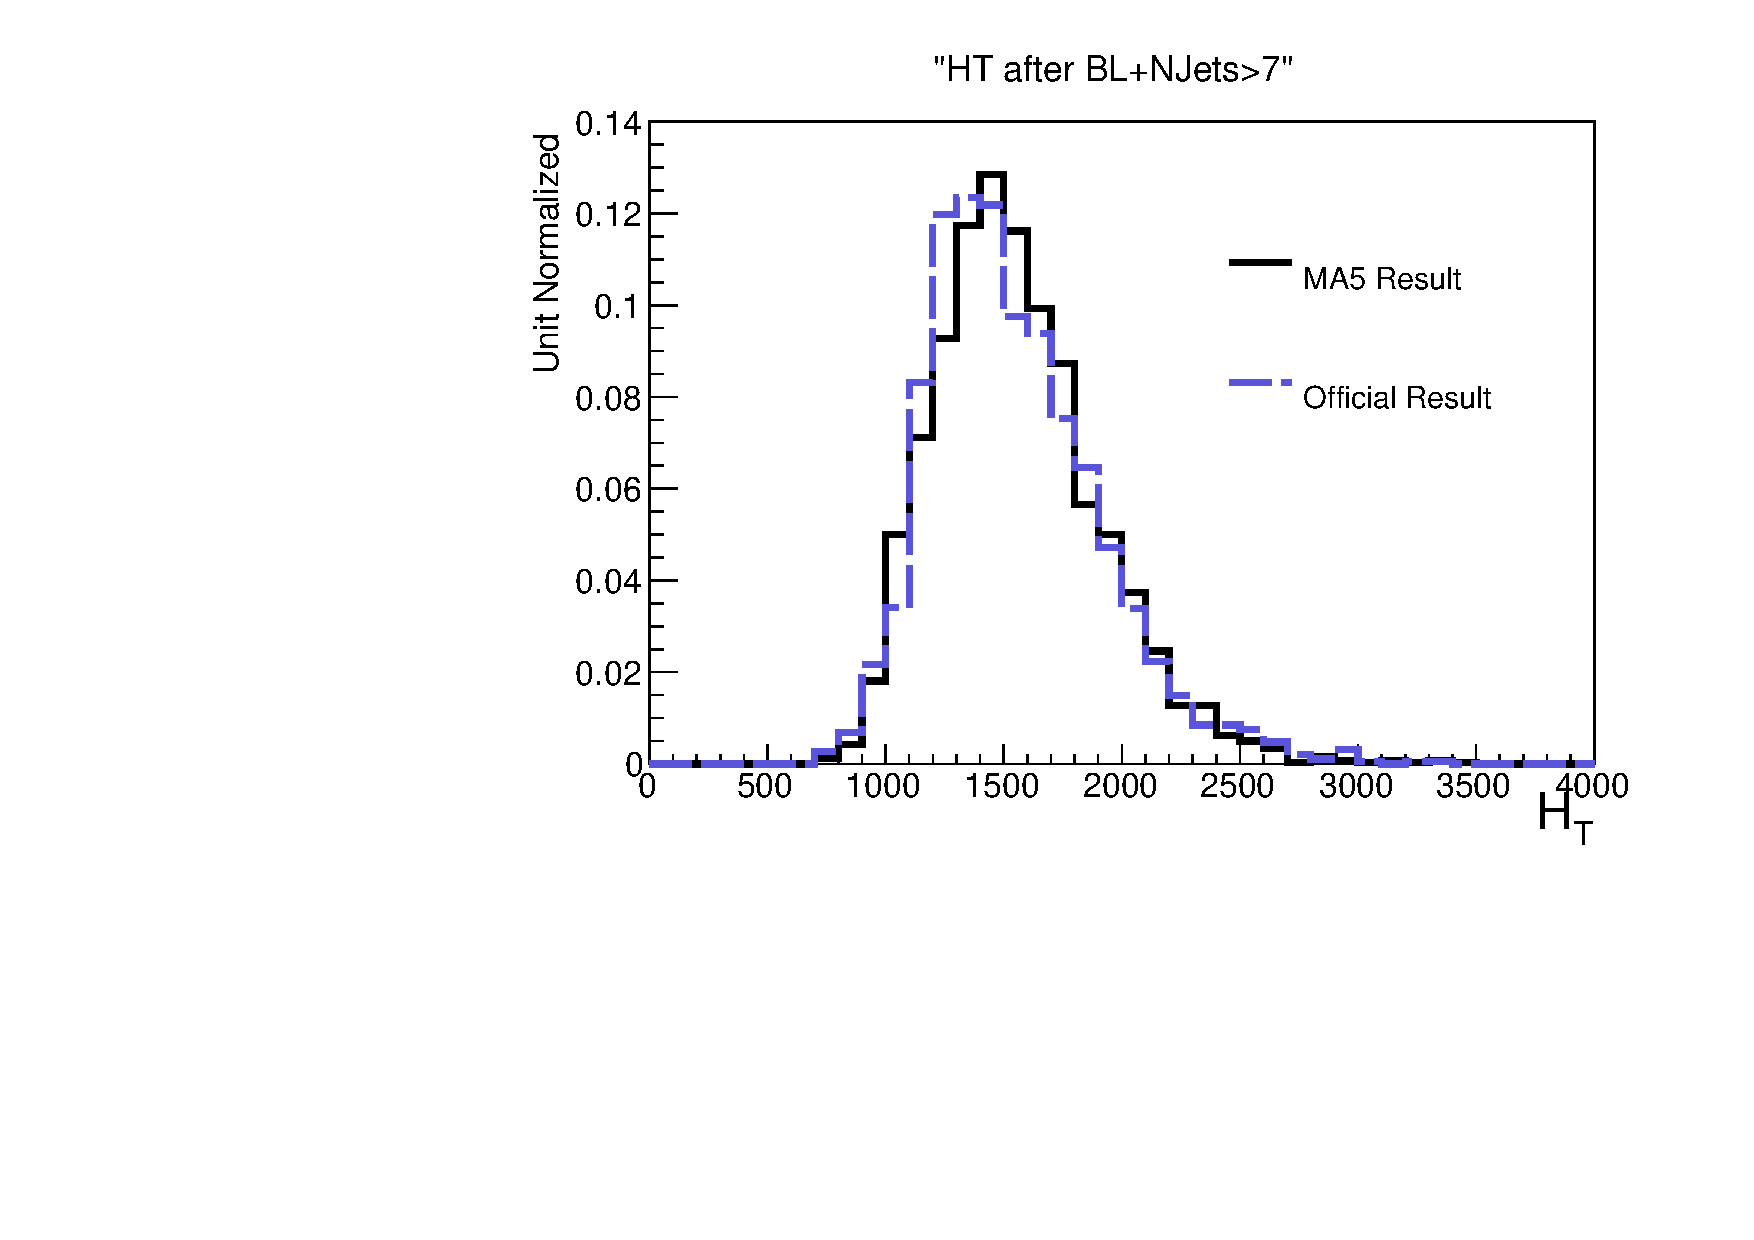
\includegraphics[width=0.5\textwidth]{figures/Appendices/Ma5ValidationSUS13012/T5VV_HT_after_BL+NJets>7.pdf}
        \label{fig:tiger}
        }
        \caption{Additional checks: comparison between ours and the official distributions of NJets after BL+$H_T$$>$1250 cuts (left), and $H_T$ after BL+NJets$>$7 cuts (right), for the T5VV signal model.}
        \end{figure}   
        

\clearpage
%%%%%%%%%%%%%%%%%%%%%%%%%%%%%%%%%%%%%%%%%%%%%%%%%
\subsubsection{T2qq simplified model}
%%%%%%%%%%%%%%%%%%%%%%%%%%%%%%%%%%%%%%%%%%%%%%%%%

\begin{figure}[h!]
\centering
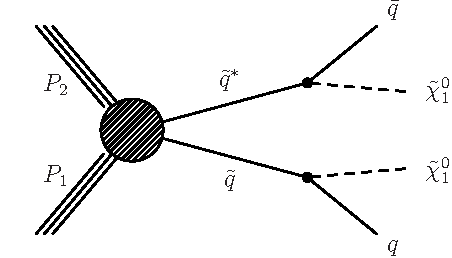
\includegraphics[width=7cm]{figures/Appendices/Ma5ValidationSUS13012/T2qq.pdf}
\caption{Diagram of the dominant SUSY production mechanism
for the T2qq signal model.}
\label{fig:T2qq}
\end{figure}

    \begin{table}[h!]
    \begin{centering}
    \begin{tabular}{  c | c | c  }
    \hline
    \hline
    Cut Name & Official Count (Eff) & MA5 Count (Eff)\\
    \hline
        MET Cleaning & 1215.2 (xxx) & 1215.2 (xxx)\\
    No Lepton & 1212.8 (99\%) & 1215.2 (100\%)\\
    NJets$>$2 & 675.9 (55\%) & 691.54 (56\%)\\
    $H_T$$>$500 & 619.5 (91\%) & 638.41 (92\%)\\
    \MHT$>$200 & 524.0 (84\%) & 539.59 (84\%)\\
    Min $\Delta(\phi)$ & 460.7 (87\%) & 476.12 (88\%)\\
\hline
\hline
    \end{tabular}
    \caption{The cut flow for the baseline selection in CMS SUS-13-012 for
    the T2qq  working point  $(m_{\tilde q},\,m_{\tilde\chi^0_1})=(700,\,100)$~GeV. 
    The second column is the official account
    and our own results are given in column 3. The official counts are
    normalized to luminosity ${\cal L}=19.5$/fb and cross section $\sigma= 63.4$~pb, and our
    counts are normalized to match the official count after the first cut, MET
    Cleaning.}
    \label{table:CF4}
    \end{centering}
    \end{table}
    
    \begin{table}
    \begin{centering}
    \begin{tabular}{  l | c | c  }
    \hline
    \hline
    Signal Region Name & Official & MA5\\
    \hline
    NJets3-5,  $H_T$500-800,  \MHT200-300 & 35.3 & 35.10\\ 
 \hline 
NJets3-5,  $H_T$500-800,  \MHT300-450 & 70.4 & 73.44\\ 
 \hline 
NJets3-5,  $H_T$500-800,  \MHT450-600 & 71.5 & 73.82\\ 
 \hline 
NJets3-5,  $H_T$500-800,  \MHT$>$600 & 23.6 & 28.78\\ 
 \hline 
NJets3-5,  $H_T$800-1000,  \MHT200-300 & 18.1 & 17.20\\ 
 \hline 
NJets3-5,  $H_T$800-1000,  \MHT300-450 & 21.9 & 32.19\\ 
 \hline 
NJets3-5,  $H_T$800-1000,  \MHT450-600 & 38.1 & 38.14\\ 
 \hline 
NJets3-5,  $H_T$800-1000,  \MHT$>$600 & 35.2 & 36.74\\ 
 \hline 
NJets3-5,  $H_T$1000-1250,  \MHT200-300 & 10.9 & 12.15\\ 
 \hline 
NJets3-5,  $H_T$1000-1250,  \MHT300-450 & 21.7 & 20.31\\ 
 \hline 
NJets3-5,  $H_T$1000-1250,  \MHT450-600 & 20.7 & 21.54\\ 
 \hline 
NJets3-5,  $H_T$1000-1250,  \MHT$>$600 & 21.8 & 23.59\\ 
 \hline 
NJets3-5,  $H_T$1250-1500,  \MHT200-300 & 4.3 & 5.53\\ 
 \hline 
NJets3-5,  $H_T$1250-1500,  \MHT300-450 & 8.1 & 7.85\\ 
 \hline 
NJets3-5,  $H_T$1250-1500,  \MHT$>$450 & 16.1 & 16.86\\ 
 \hline 
NJets3-5,  $H_T$$>$1500,  \MHT200-300 & 3.7 & 3.68\\ 
 \hline 
NJets3-5,  $H_T$$>$1500,  \MHT$>$300 & 13. & 13.45\\ 
 \hline 
NJets6-7,  $H_T$500-800,  \MHT200-300 & 0.8 & 0.40\\ 
 \hline 
NJets6-7,  $H_T$500-800,  \MHT300-450 & 1.0 & 0.44\\ 
 \hline 
NJets6-7,  $H_T$500-800,  \MHT$>$450 & 0.4 & 0.44\\ 
 \hline 
NJets6-7,  $H_T$800-1000,  \MHT200-300 & 0.5 & 0.58\\ 
 \hline 
NJets6-7,  $H_T$800-1000,  \MHT300-450 & 1.1 & 1.26\\ 
 \hline 
NJets6-7,  $H_T$800-1000,  \MHT$>$450 & 1.5 & 1.63\\ 
 \hline 
NJets6-7,  $H_T$1000-1250,  \MHT200-300 & 1.0 & 0.61\\ 
 \hline 
NJets6-7,  $H_T$1000-1250,  \MHT300-450 & 1.2 & 1.33\\ 
 \hline 
NJets6-7,  $H_T$1000-1250,  \MHT$>$450 & 2.5 & 3.24\\ 
 \hline 
NJets6-7,  $H_T$1250-1500,  \MHT200-300 & 0.6 & 0.61\\ 
 \hline 
NJets6-7,  $H_T$1250-1500,  \MHT300-450 & 1.2 & 0.61\\ 
 \hline 
NJets6-7,  $H_T$1250-1500,  \MHT$>$450 & 1.4 & 1.84\\ 
 \hline 
NJets6-7,  $H_T$$>$1500,  \MHT200-300 & 0.6 & 0.30\\ 
 \hline 
NJets6-7,  $H_T$$>$1500,  \MHT$>$300 & 2.3 & 1.80\\ 
 \hline 
NJets$>$7,  $H_T$500-800,  \MHT$>$200 & 0.0 & 0.0\\ 
 \hline 
NJets$>$7,  $H_T$800-1000,  \MHT$>$200 & 0.0 & 0.0\\ 
 \hline 
NJets$>$7,  $H_T$1000-1250,  \MHT$>$200 & 0.2 & 0.27\\ 
 \hline 
NJets$>$7,  $H_T$1250-1500,  \MHT$>$200 & 0.3 & 0.10\\ 
 \hline 
NJets$>$7,  $H_T$$>$1500,  \MHT$>$200 & 0.3 & 0.13\\ 
 \hline 
\hline
    \end{tabular}
    \caption{The signal region (SR) counts in CMS SUS-13-012 for the T2qq scenario 
    after all selection has been applied. Column 2 is the official account obtained through generous correspondence with Christian Sanders,
    and our own results displayed in column 3. These counts were determined by applying the SR selection to the end of the cut flow featured in table \ref{table:CF4}.}
    \label{table:last}
    \end{centering}
    \end{table}
    
\begin{figure}
        \centering
        \subfloat[]{
                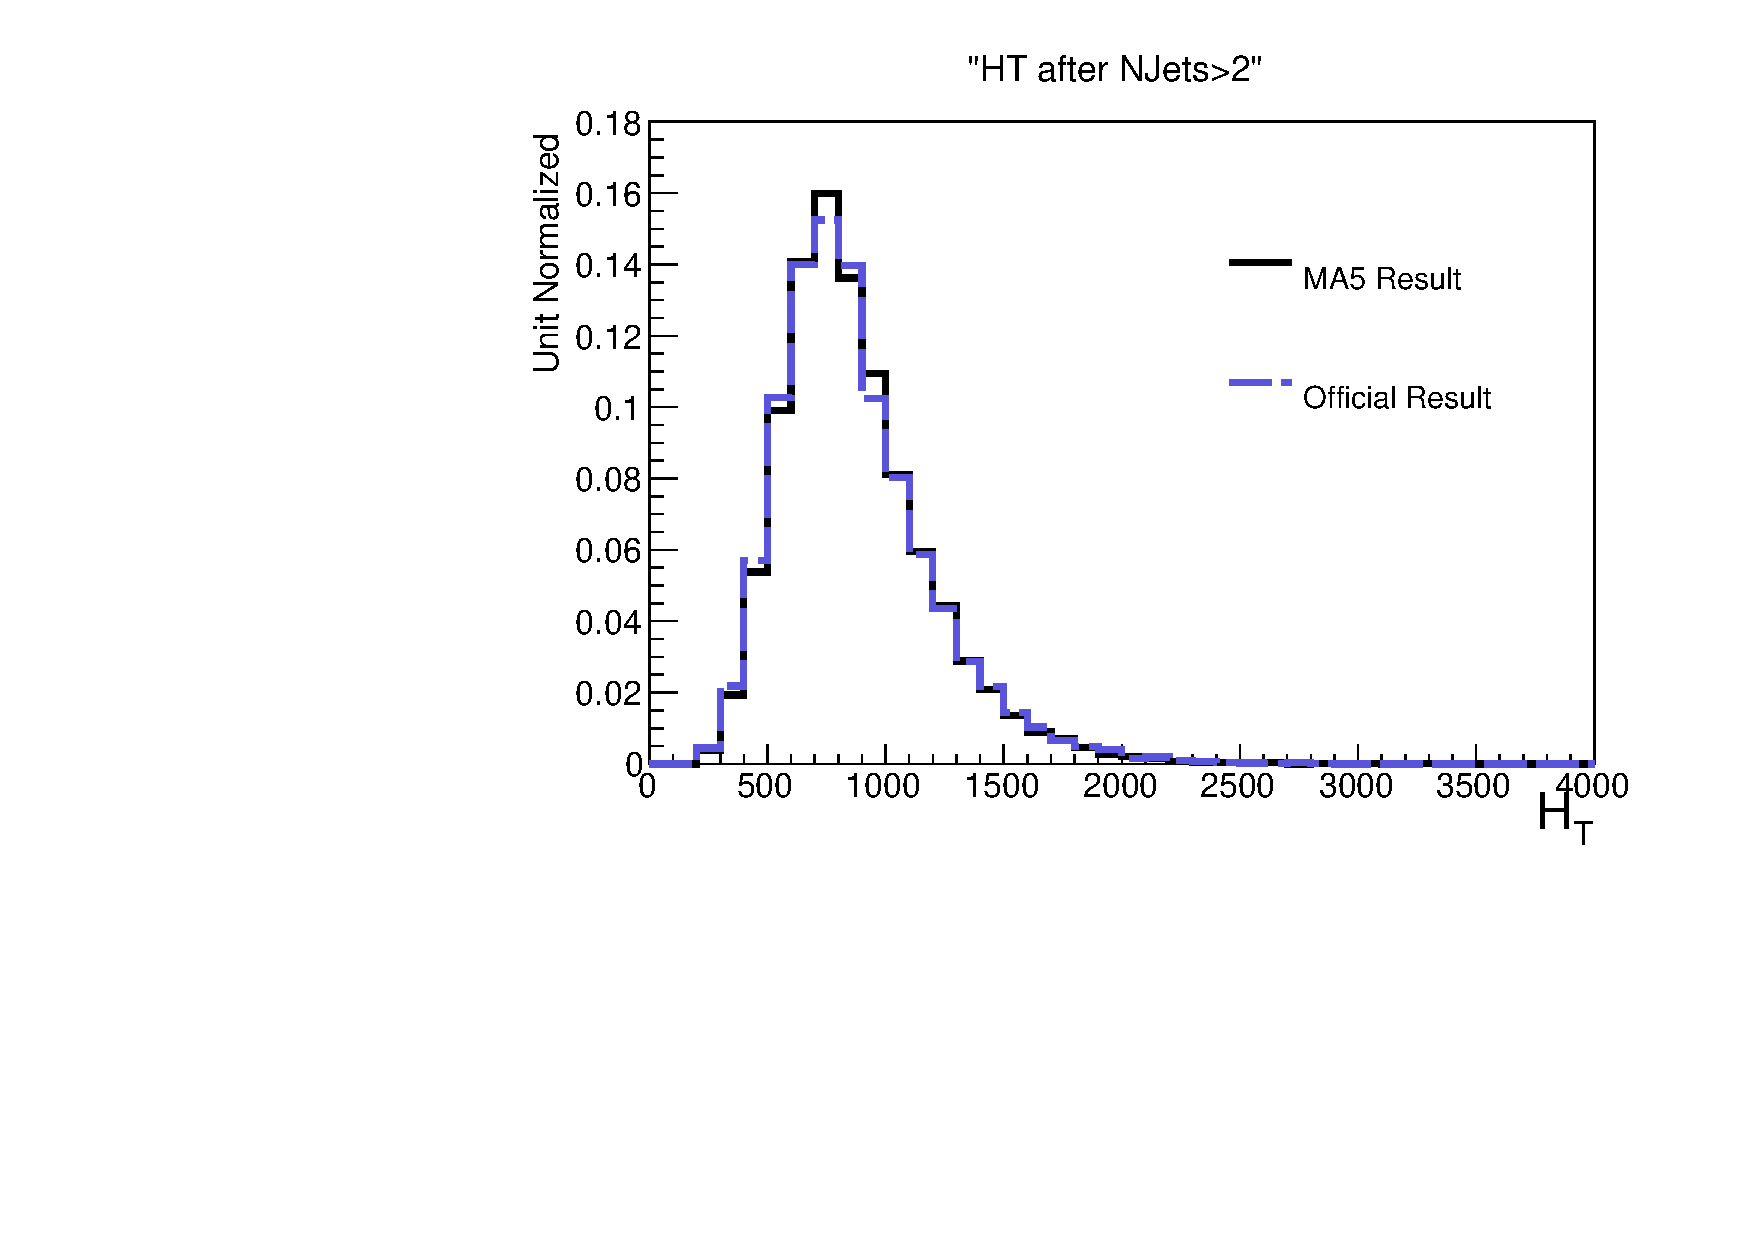
\includegraphics[width=0.5\textwidth]{figures/Appendices/Ma5ValidationSUS13012/T2qq_HT_after_NJets>2.pdf}
                \label{fig:gull}
        }%
        \hspace{-1 cm}
        ~ %add desired spacing between images, e. g. ~, \quad, \qquad, \hfill etc.
          %(or a blank line to force the subfigure onto a new line)
        \subfloat[]{
                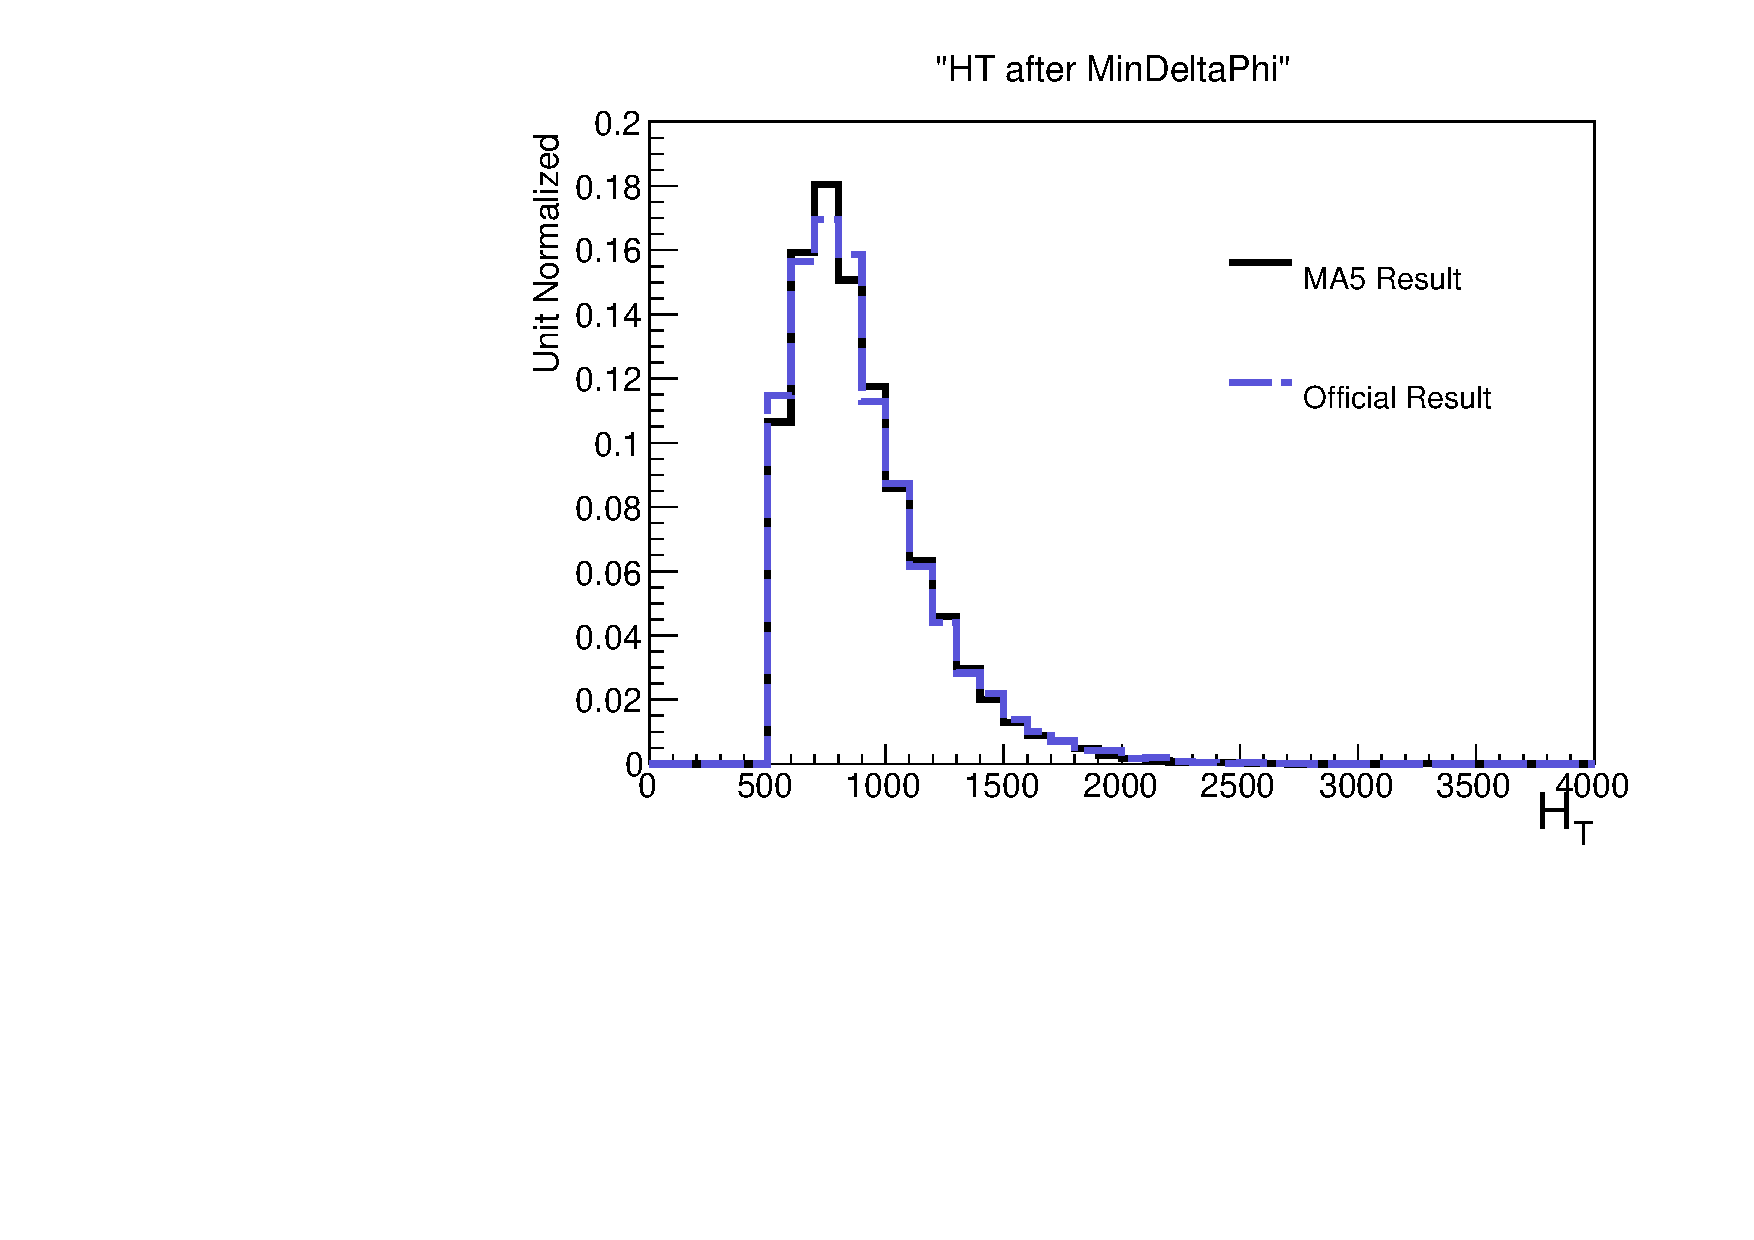
\includegraphics[width=0.5\textwidth]{figures/Appendices/Ma5ValidationSUS13012/T2qq_HT_after_MinDeltaPhi.pdf}
                \label{fig:tiger}
        }
        \caption{Comparison of the distributions of $H_T$ between the official and our own samples after the ``n-1" cut, Min $\Delta(\phi)$ (left), and after all baseline cuts (right), for the T2qq signal model.}\label{fig:animals}
\end{figure}        
        
\begin{figure}
        \centering
        \subfloat[]{
                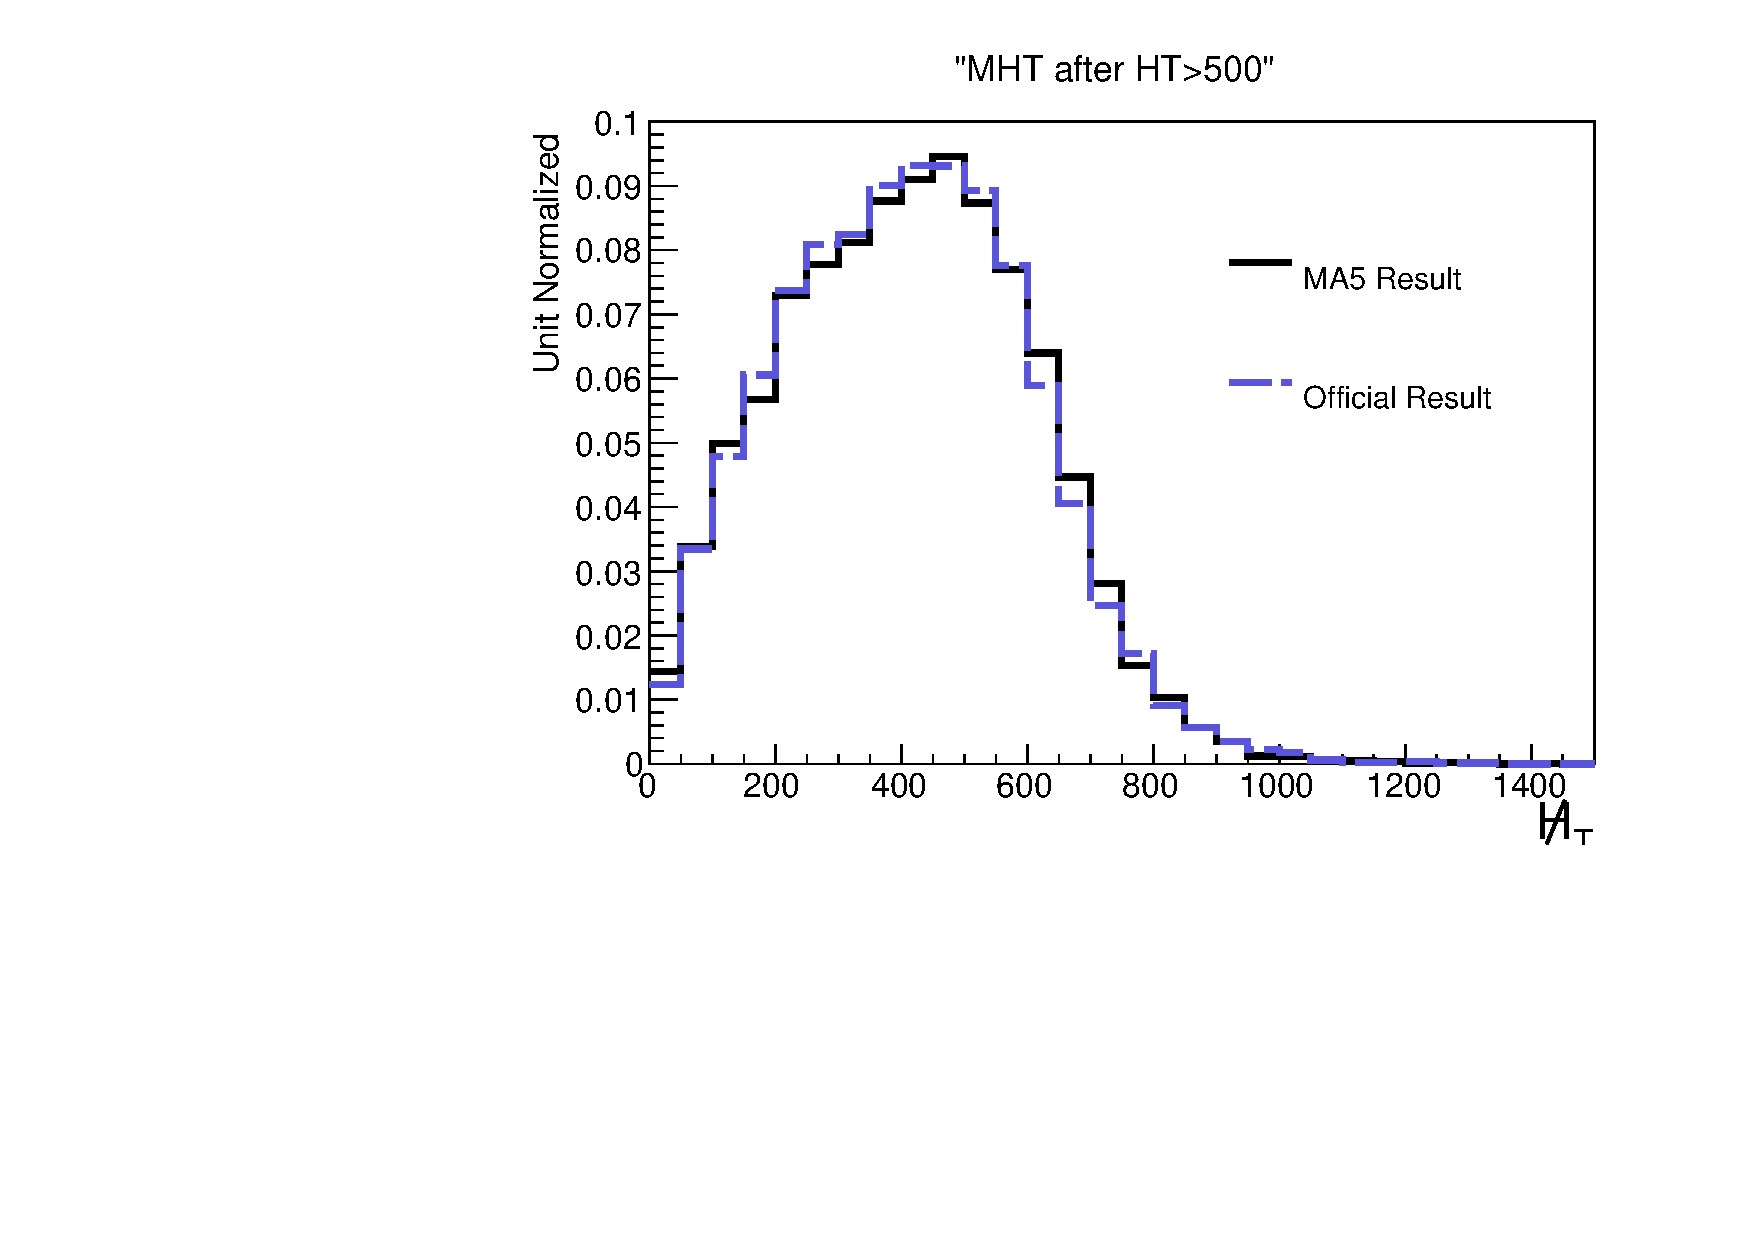
\includegraphics[width=0.5\textwidth]{figures/Appendices/Ma5ValidationSUS13012/T2qq_MHT_after_HT>500.pdf}
                \label{fig:gull}
        }%
        \hspace{-1 cm}
        ~ %add desired spacing between images, e. g. ~, \quad, \qquad, \hfill etc.
          %(or a blank line to force the subfigure onto a new line)
        \subfloat[]{
                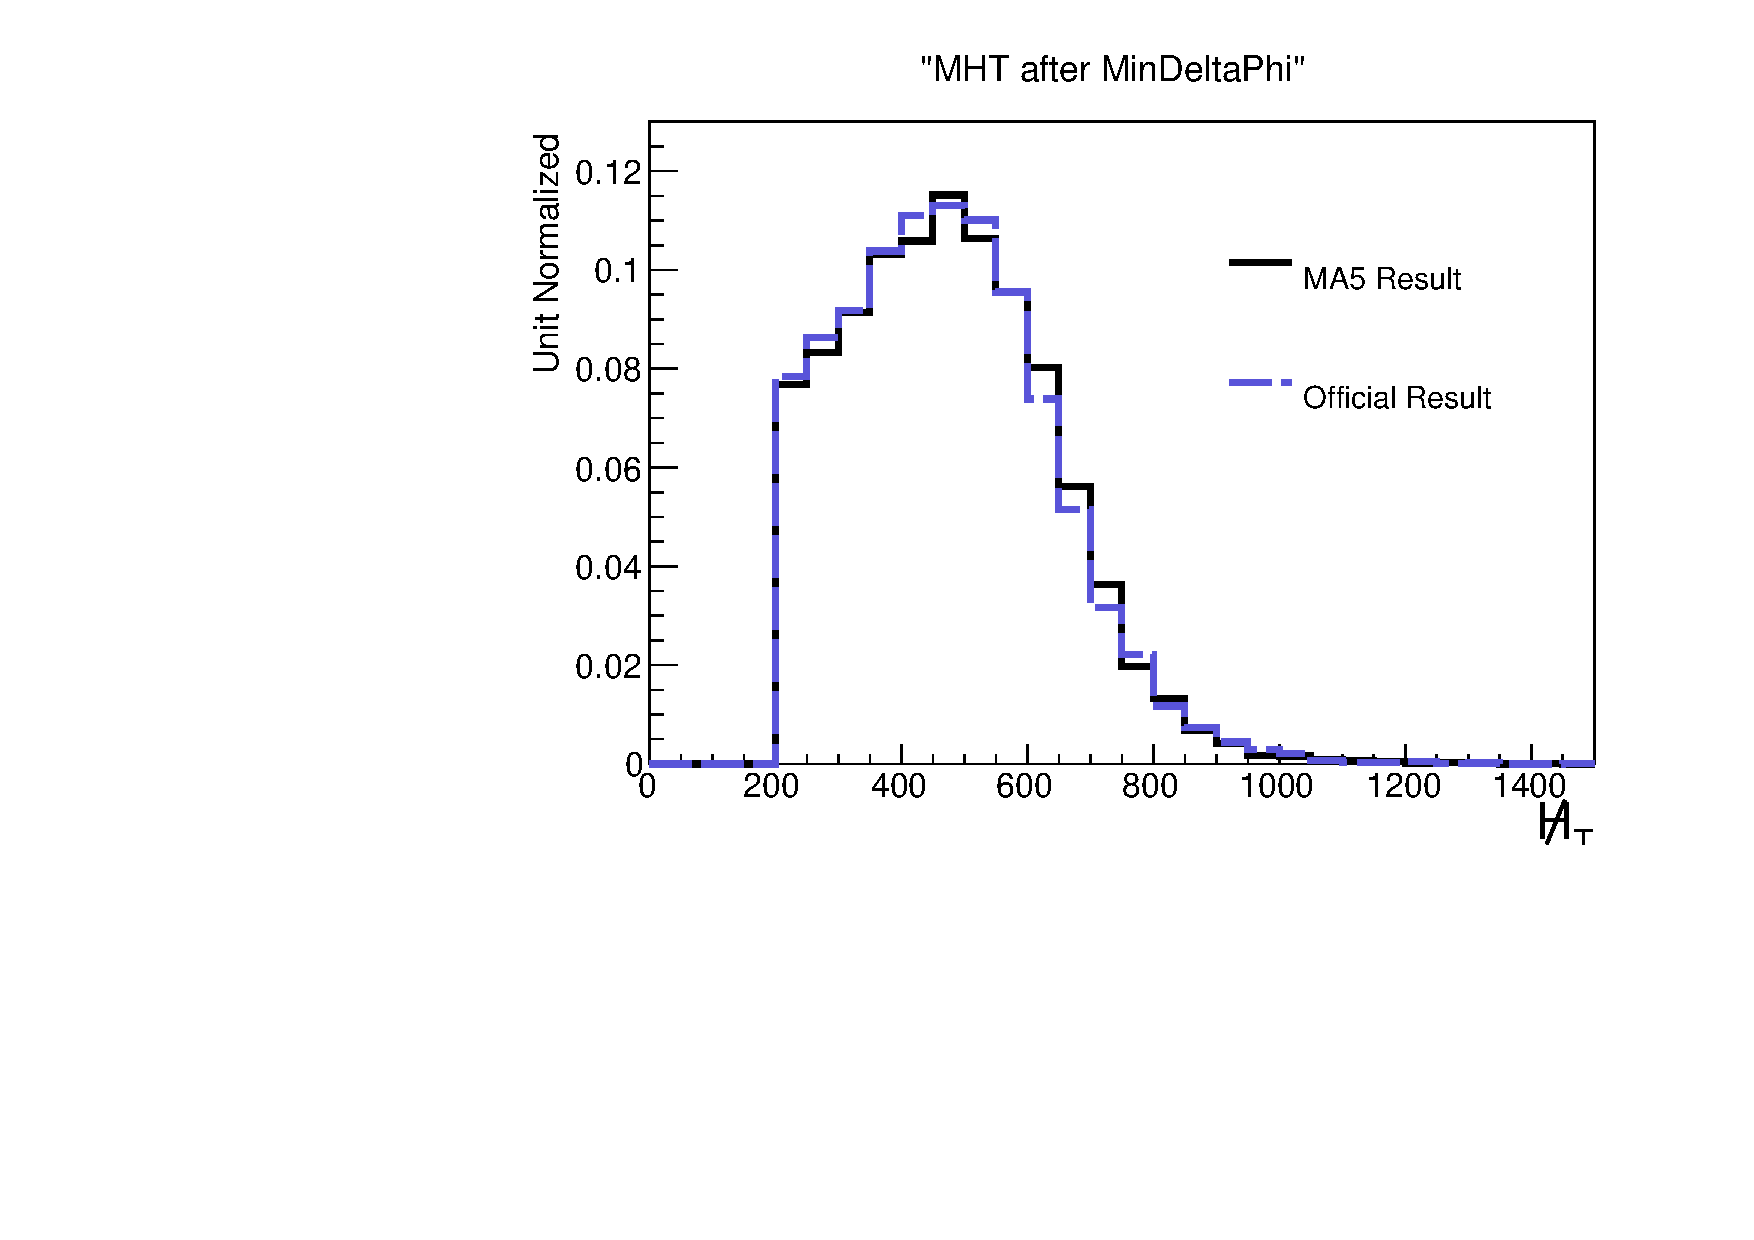
\includegraphics[width=0.5\textwidth]{figures/Appendices/Ma5ValidationSUS13012/T2qq_MHT_after_MinDeltaPhi.pdf}
                \label{fig:tiger}
        }
        \caption{Comparison of the distributions of \MHT between the official and our own samples after the ``n-1" cut, Min $\Delta(\phi)$ (left), and after all baseline cuts (right), for the T2qq signal model.}\label{fig:animals}
\end{figure}        
        
\begin{figure}
        \centering
        \subfloat[]{
                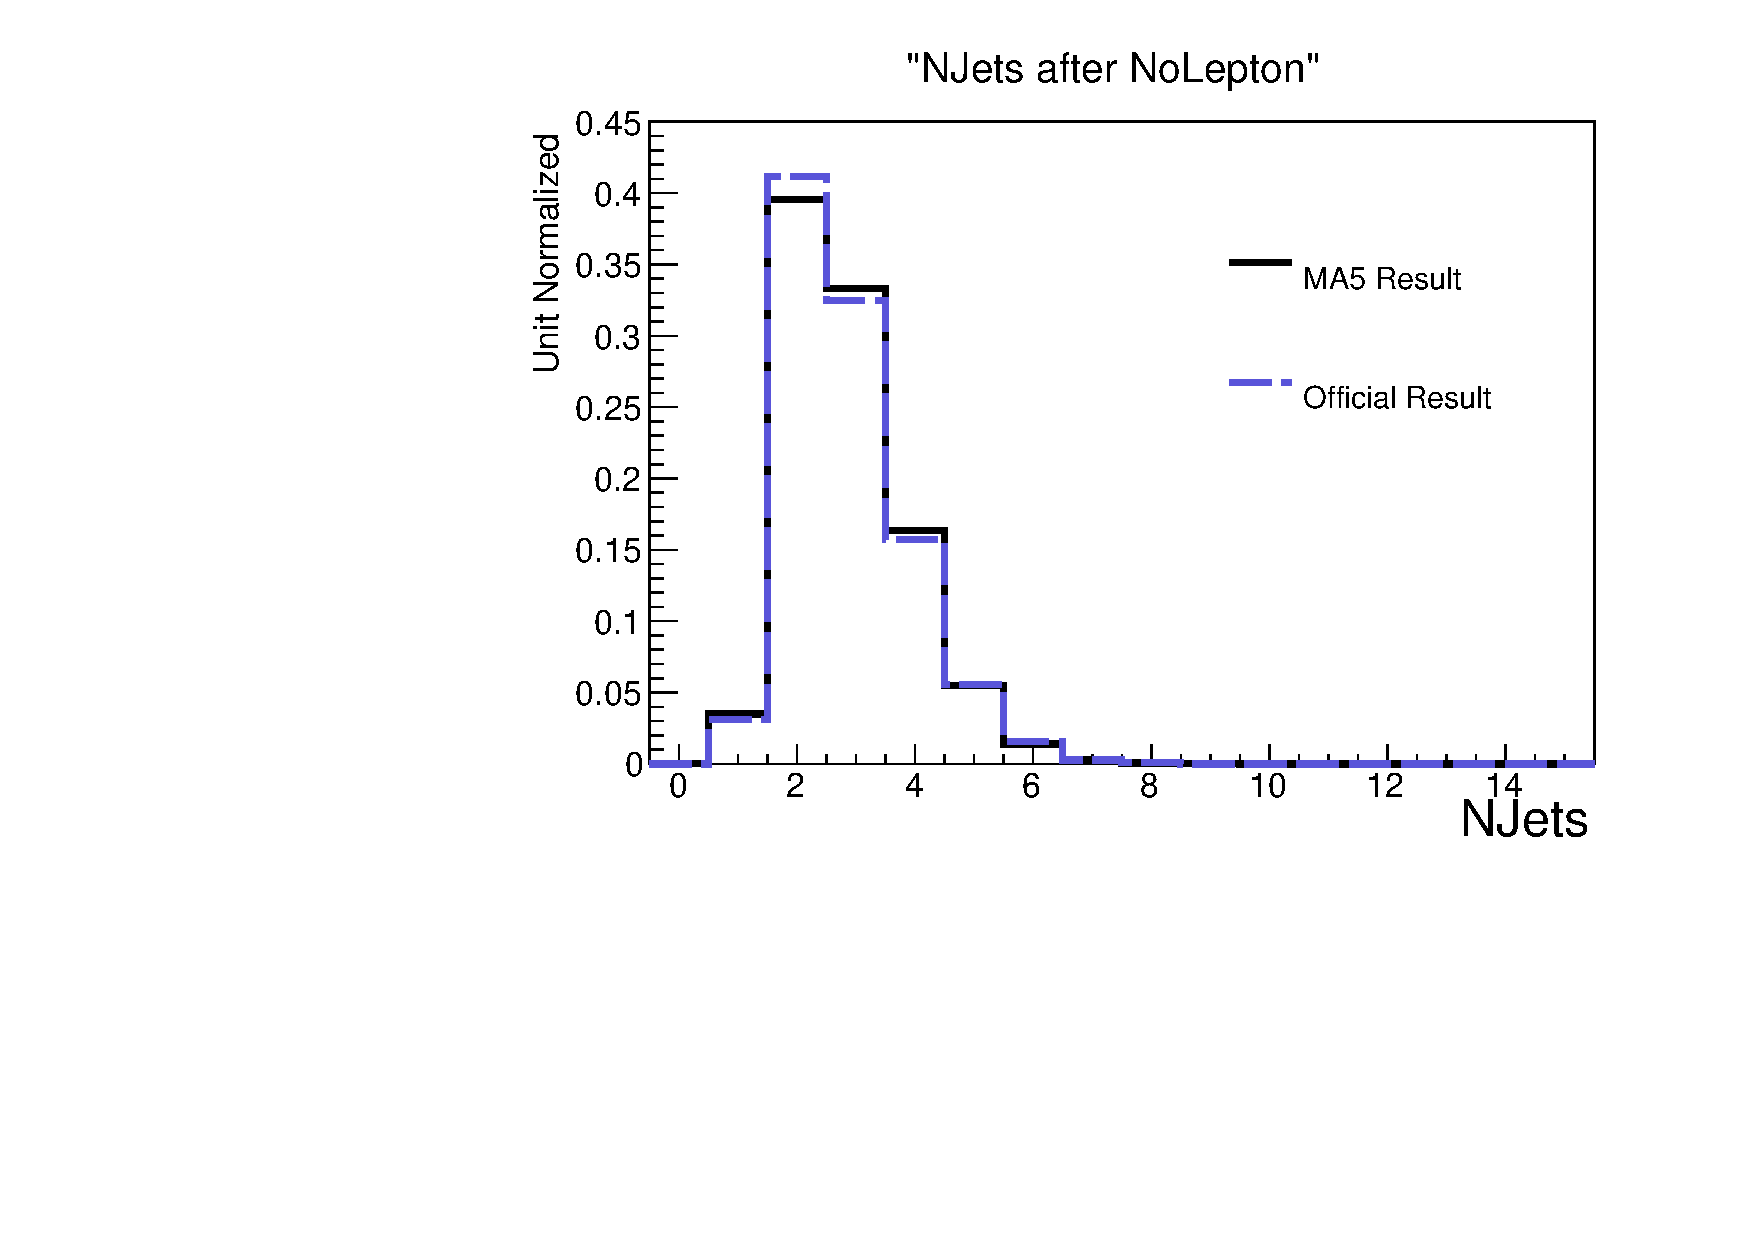
\includegraphics[width=0.5\textwidth]{figures/Appendices/Ma5ValidationSUS13012/T2qq_NJets_after_NoLepton.pdf}
                \label{fig:gull}
        }%
        \hspace{-1 cm}
        ~ %add desired spacing between images, e. g. ~, \quad, \qquad, \hfill etc.
          %(or a blank line to force the subfigure onto a new line)
        \subfloat[]{
                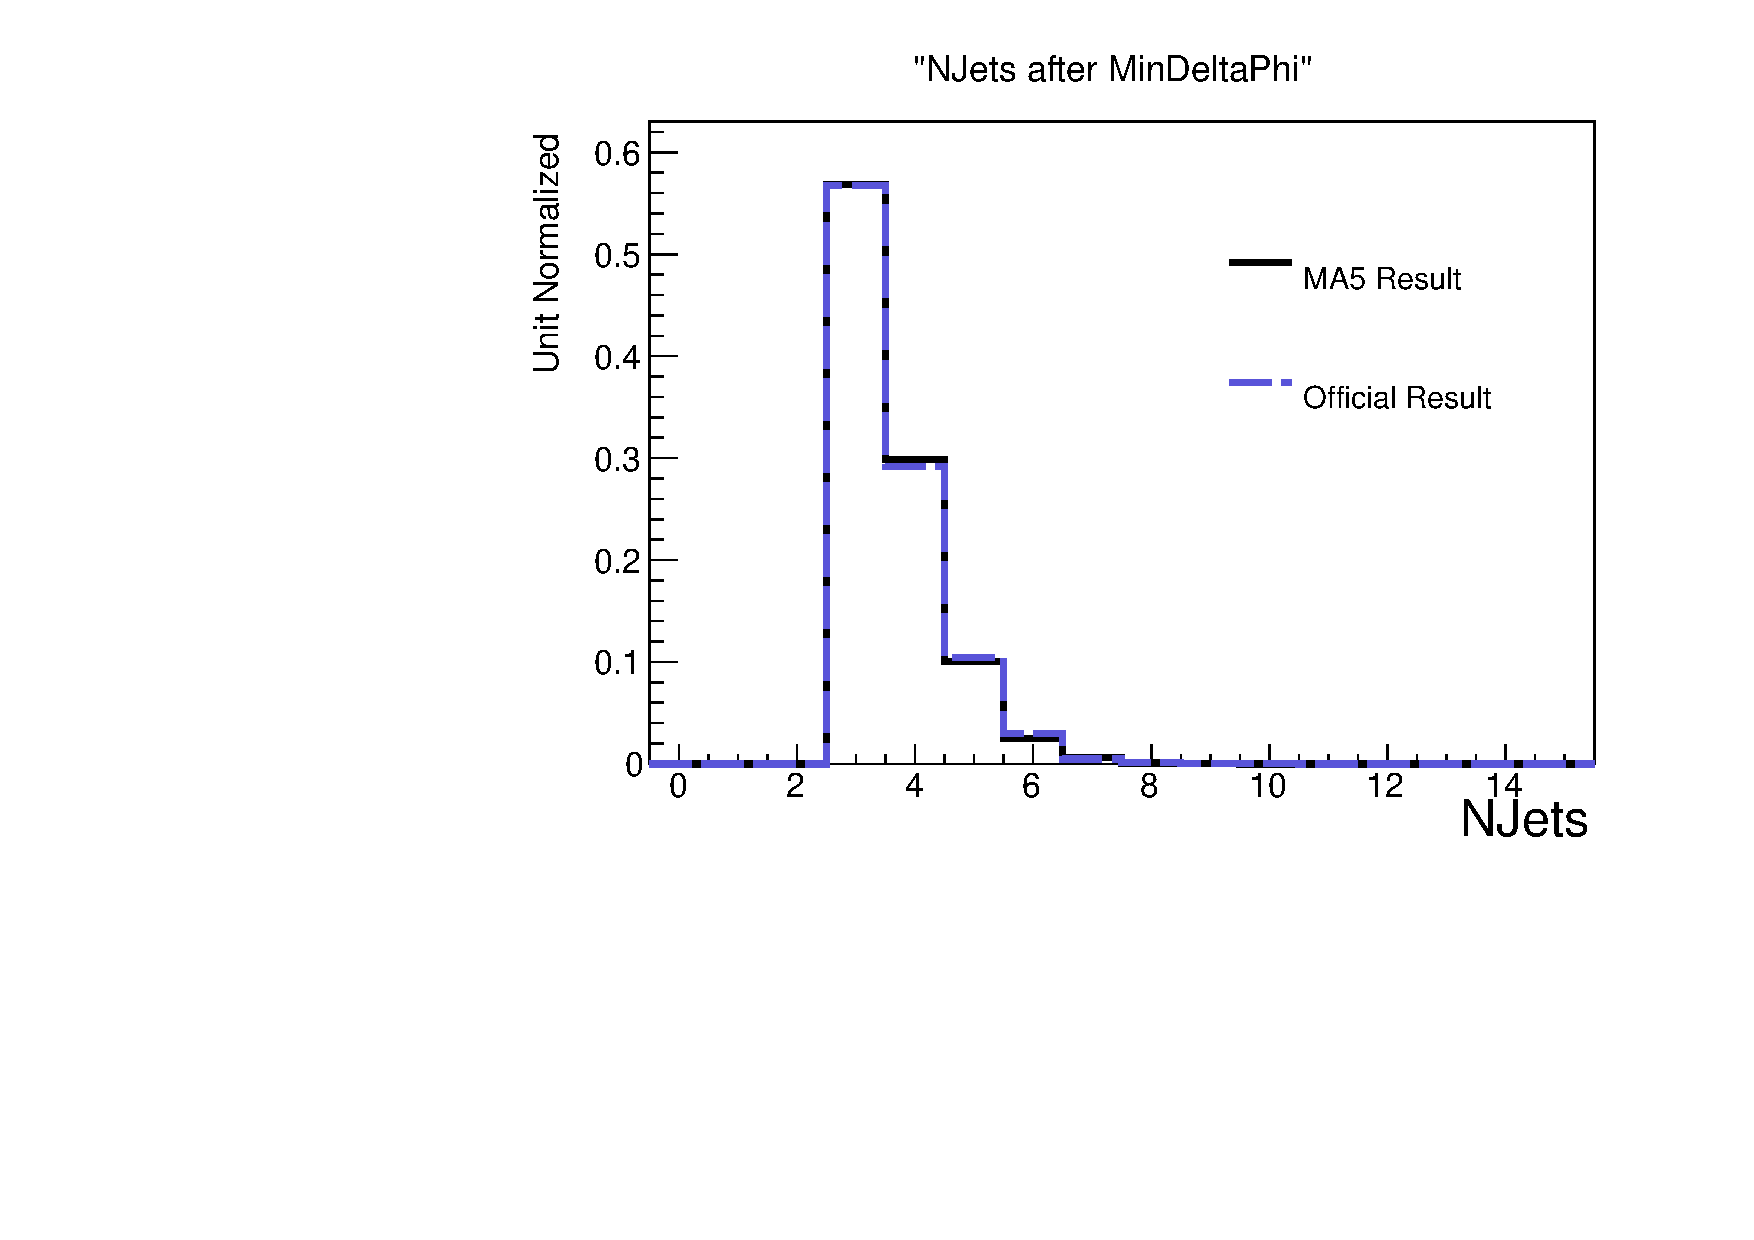
\includegraphics[width=0.5\textwidth]{figures/Appendices/Ma5ValidationSUS13012/T2qq_NJets_after_MinDeltaPhi.pdf}
                \label{fig:tiger}
        }
        \caption{Comparison of the distributions of NJets between the official and our own samples after the ``n-1" cut, Min $\Delta(\phi)$ (left), and after all baseline cuts (right), for the T2qq signal model.}\label{fig:animals}
\end{figure}        
        
        \begin{figure}
        \centering
        \subfloat[]{
        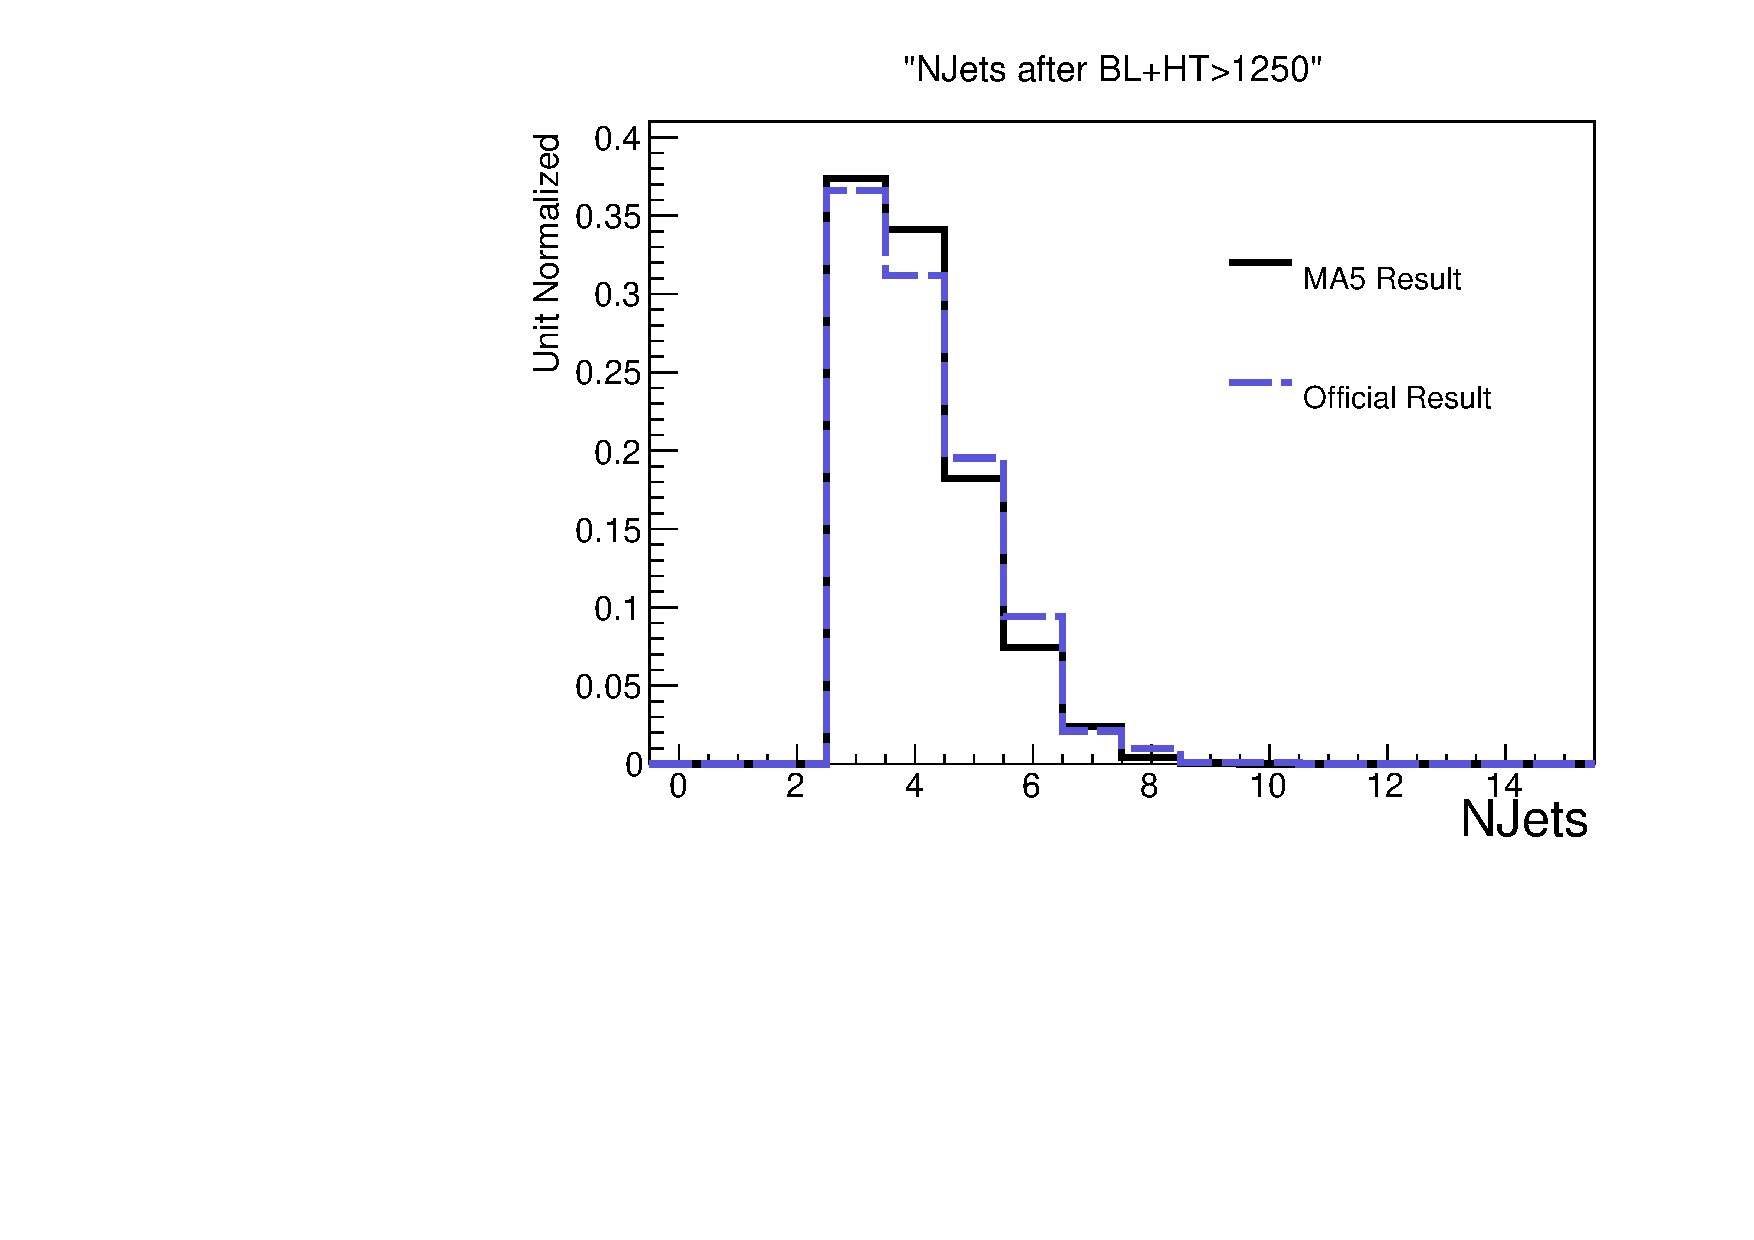
\includegraphics[width=0.5\textwidth]{figures/Appendices/Ma5ValidationSUS13012/T2qq_NJets_after_BL+HT>1250.pdf}
        \label{fig:gull}
        }%
        \hspace{-1 cm}
        ~ %add desired spacing between images, e. g. ~, \quad, \qquad, \hfill etc.
        %(or a blank line to force the subfigure onto a new line)
        \subfloat[]{
        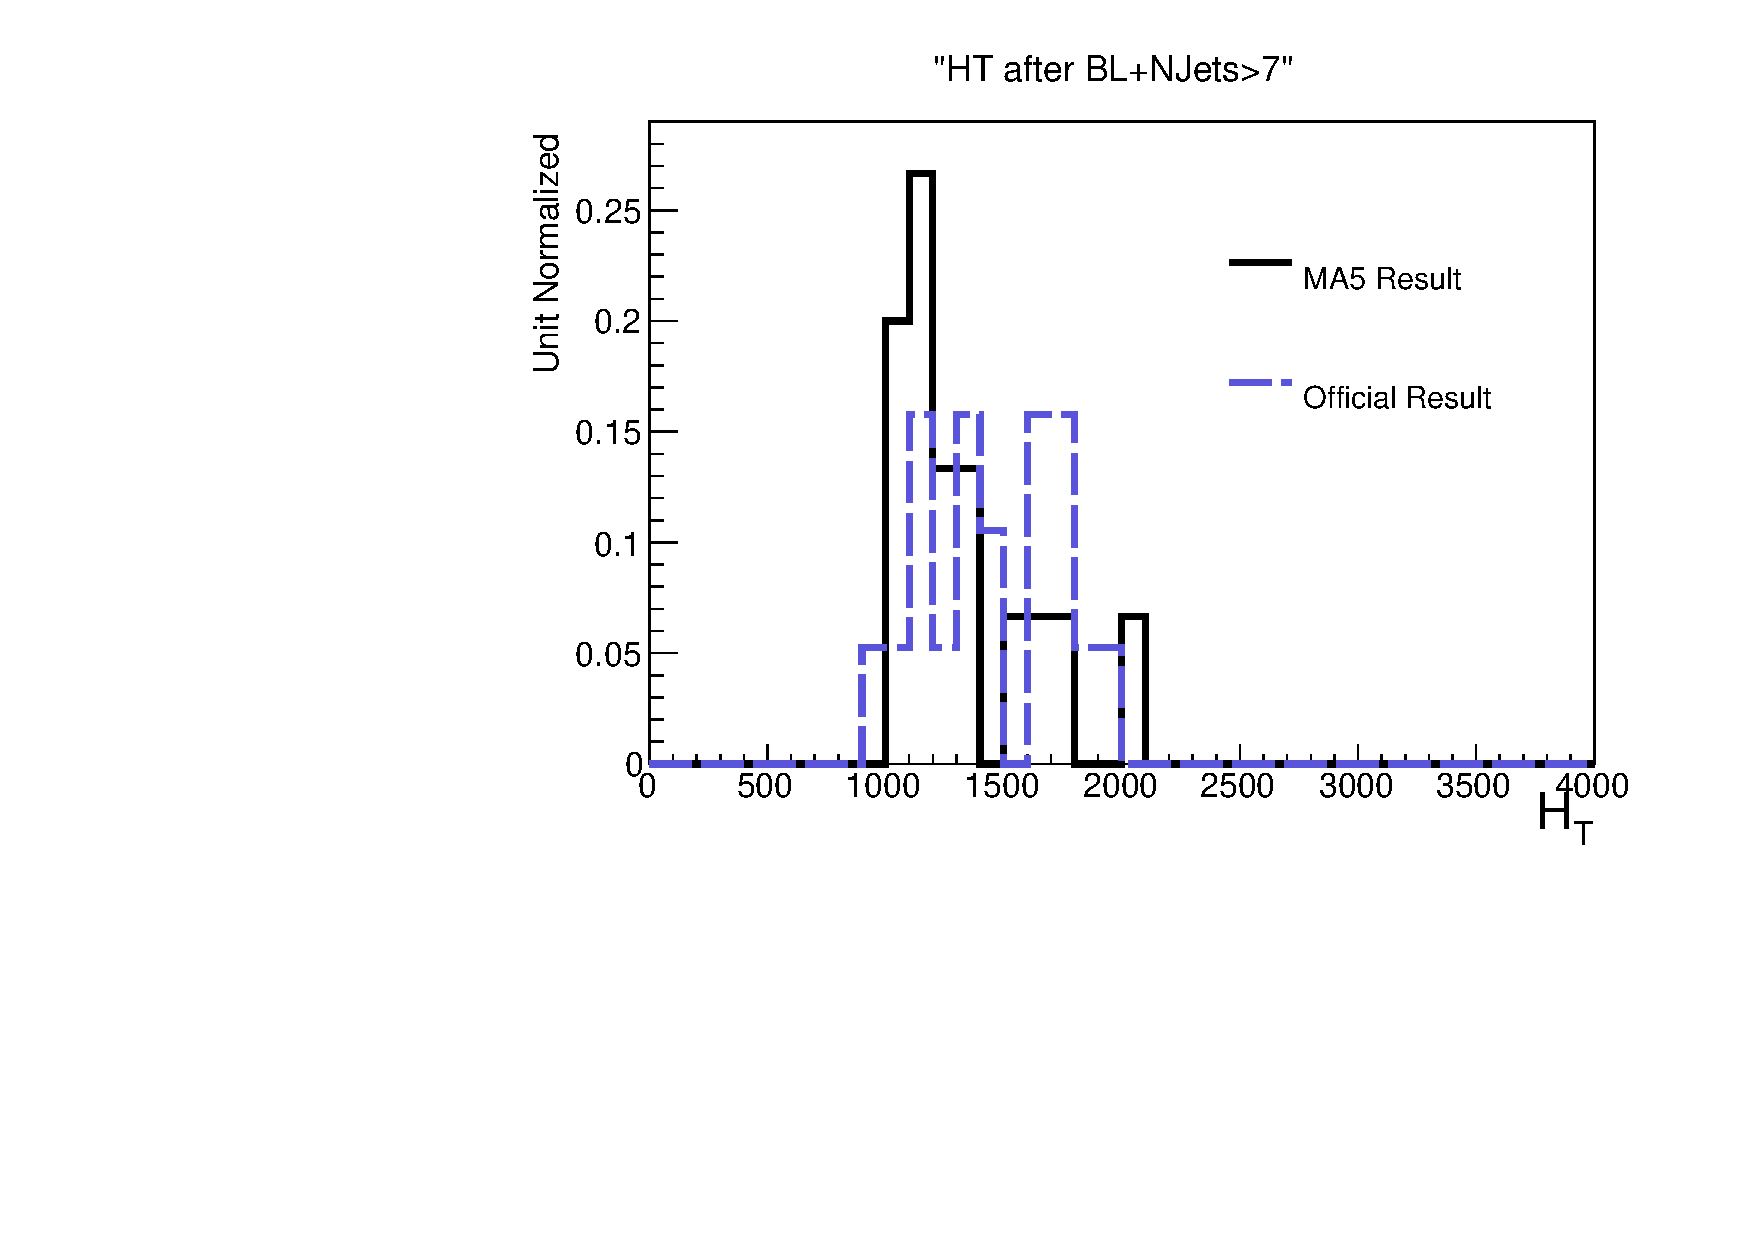
\includegraphics[width=0.5\textwidth]{figures/Appendices/Ma5ValidationSUS13012/T2qq_HT_after_BL+NJets>7.pdf}
        \label{fig:tiger}
        }
        \caption{Additional checks: comparison between ours and the official distributions of NJets after BL+$H_T$$>$1250 cuts (left), and $H_T$ after BL+NJets$>$7 cuts (right), for the T2qq signal model.}
        \label{fig:last}
        \end{figure} 
        
        
\clearpage
%%%%%%%%%%%%%%%%%%%%%%%%%%%%%%%%%%%%%%%%%%%%%%%%%
\subsubsection{Exclusion Limits}
%%%%%%%%%%%%%%%%%%%%%%%%%%%%%%%%%%%%%%%%%%%%%%%%%

It is also instructive to reproduce the 95\%~CL exclusion lines in the $(m_{\tilde g},\,m_{\tilde\chi^0_1})$ 
and $(m_{\tilde q},\,m_{\tilde\chi^0_1})$ mass planes.  
% for the four benchmark scenarios, T1tttt ($\tilde{g}\to t\bar{t}\chi_{1}^{0}$),
%T2qq ($\tilde{q}\to q \chi_{1}^{0} $), T1qqqq ($\tilde{g}\to q\bar{q}\chi_{1}^{0}$),
%and T5VV ($\tilde{g} \to q\bar{q}V\chi_{1}^{0}$). 
Figure~\ref{fig:limitplots}  shows the limit curves (in red) obtained with our 
{\sc{MadAnalysis}}~5 implementation and using the {\tt{exclusion\_CLs.py}} code described in 
\href{http://arxiv.org/abs/arXiv:1407.3278}{arXiv:1407.3278} 
superimposed on the official CMS exclusion with its $\pm 1\sigma$ theoretical uncertainty (solid and dashed black lines).  For the T1qqqq ($\tilde{g}\to q\bar{q}\chi_{1}^{0}$) and T5VV ($\tilde{g} \to q\bar{q}V\chi_{1}^{0}$) simplified models, the limits are reproduced very well. 
Also for T1tttt ($\tilde{g}\to t\bar{t}\chi_{1}^{0}$) the agreement is reasonably fine. 
For T2qq ($\tilde{q}\to q \chi_{1}^{0} $), however, we encounter a rather erratic behavior for 
LSP masses above about 200--250~GeV.

It should be noted that our limit setting procedure differs from that used by CMS, and so should be 
considered a rough estimate. Our procedure is as follows. For any given point
on the mass plane, the production cross section is taken from the LHC SUSY cross sections twiki 
and the signal acceptance is computed with our {\sc{MadAnalysis}}~5 recast code for the analysis.
Then, the most sensitive signal region (SR), out of the 36 total SRs, is determined based on the 
number of expected signal and background counts. 
Finally, the CLs exclusion value is determined from the expected signal, expected
background, expected uncertainty on the background, and observed counts in the most sensitive
SR. 

The primary difference between our method and that used by CMS is that we consider only the most sensitive SR
in the exclusion calculation, whereas CMS uses all signal regions simultaneously and considers correlations
in the uncertainty between signal regions. This difference introduces a certain volatility in our  
exclusion limits, which can however be mitigated by demanding that jumps in exclsusion between two 
neighbouring points close in mass be not too large. 
As can be seen in Fig.!\ref{fig:limitplots}, we obtain excellent results for the T1qqqq and T5VV scenarios; the 
exclusion curve for T1tttt shows more fluctuations but none the less matches the official result reasonably well. 
The only problematic case is the T2qq topology with LSP masses above 200--250~GeV: here our procedure 
clearly does not well reproduce the official limit curve. To improve the situation, we would need the  
statistical model from CMS for combining  the 36 SRs. Unfortunately, this is currently not available.   

 \begin{figure}
        \centering
        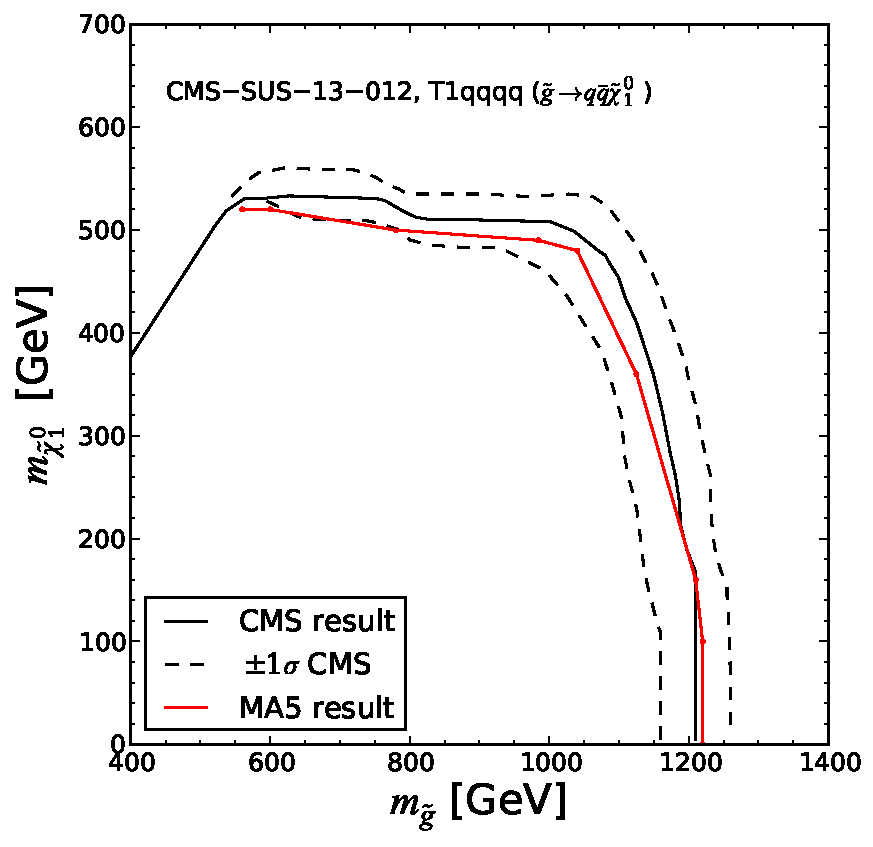
\includegraphics[width=0.48\textwidth]{figures/Appendices/Ma5ValidationSUS13012/cms-012-limit-T1qqqq.pdf}
        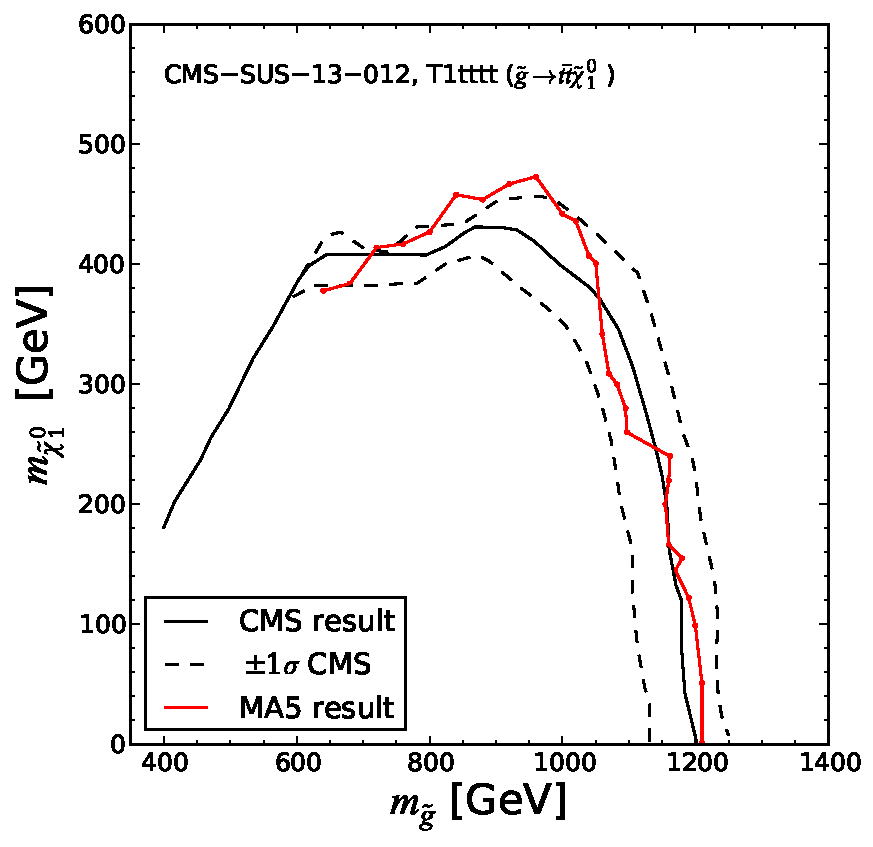
\includegraphics[width=0.48\textwidth]{figures/Appendices/Ma5ValidationSUS13012/cms-012-limit-T1tttt.pdf}\\
        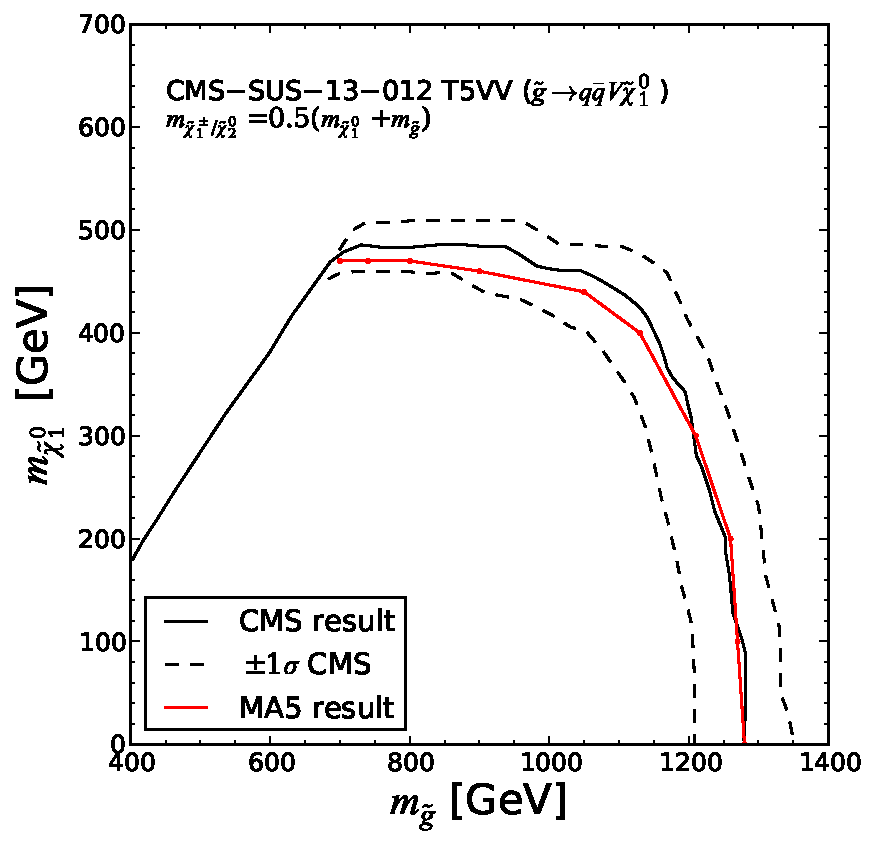
\includegraphics[width=0.48\textwidth]{figures/Appendices/Ma5ValidationSUS13012/cms-012-limit-T5VV.pdf}
        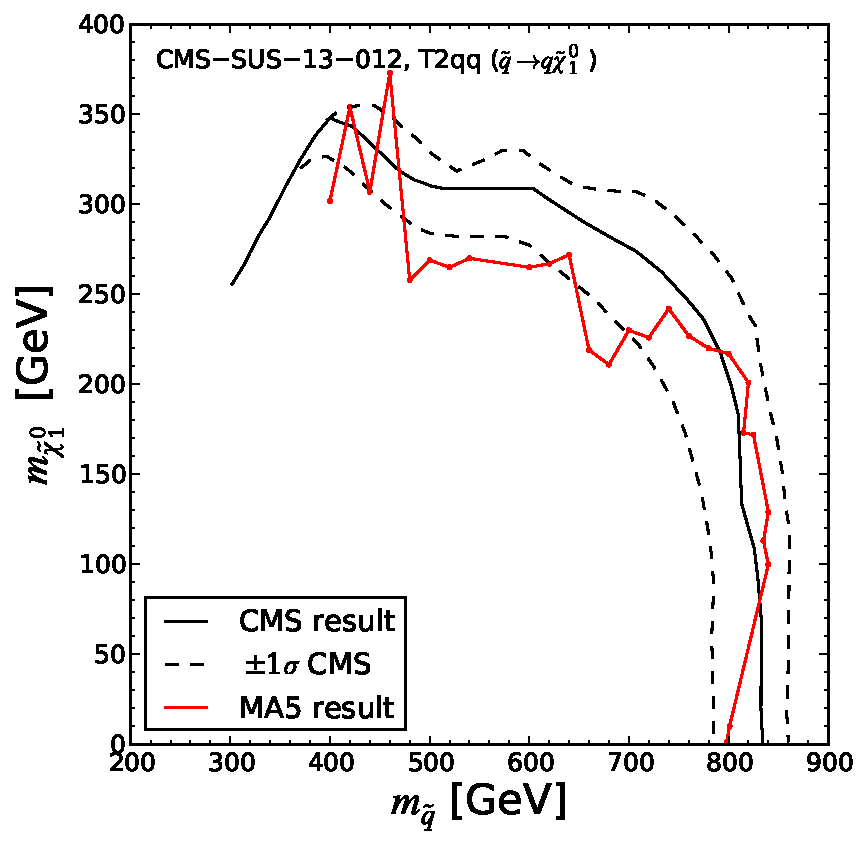
\includegraphics[width=0.48\textwidth]{figures/Appendices/Ma5ValidationSUS13012/cms-012-limit-T2qq.pdf}
\caption{The 95\% CL exclusion limits (in red) reproduced with our {\sc{MadAnalysis}}~5 implementation compared to the official limits (in black). Top left: T1qqqq, top right: T1tttt, bottom left: T5VV, bottom right: T2qq simplified models.
\label{fig:limitplots}}
        \end{figure} 
